\chapter{Phân tích và thiết kế hệ thống}
\label{chap:2}

Chương này trình bày kết quả phân tích yêu cầu và thiết kế của ứng dụng ngân hàng di động Nene theo yêu cầu báo cáo TR-05 của đề bài: biểu đồ ca sử dụng, kiến trúc thành phần và hạ tầng, lý do lựa chọn công nghệ, các nguyên tắc và mẫu thiết kế được áp dụng, biểu đồ lớp, thiết kế cơ sở dữ liệu và các luồng xử lý quan trọng. Mọi sơ đồ và mô tả trong chương được đối chiếu trực tiếp với mã nguồn trên nhánh \texttt{main} tại commit \texttt{2b0aa73}: backend trong \texttt{backend/\allowbreak{}src}, ứng dụng Flutter trong \texttt{app/\allowbreak{}lib} và 17 tệp migration SQL trong \texttt{infrastructure/\allowbreak{}supabase/\allowbreak{}migrations}. Nhóm chỉ mô tả hành vi đã có trong mã; những phần là mô phỏng, dữ liệu hư cấu hoặc môi trường thử nghiệm (sandbox) được ghi nhãn rõ ràng ngay tại chỗ.

% ======================================================================
\section{Phân tích yêu cầu}
\label{sec:ch2-requirements}

Từ bảy nhóm nghiệp vụ trong đề bài, nhóm lập một sổ yêu cầu gồm các yêu cầu nghiệp vụ BR-01 đến BR-14 và yêu cầu kỹ thuật TR-01 đến TR-08. Mỗi yêu cầu được gắn với vị trí trong đề bài và tiêu chí nghiệm thu, nhờ đó mọi quyết định thiết kế ở các mục sau có thể truy vết ngược về đúng yêu cầu gốc. Bảng~\ref{tab:ch2-br} tóm tắt các yêu cầu liên quan trực tiếp đến thiết kế và mức đáp ứng thực tế của hệ thống.

{\small
\begin{longtable}{>{\raggedright\arraybackslash}p{0.09\textwidth}>{\raggedright\arraybackslash}p{0.41\textwidth}>{\raggedright\arraybackslash}p{0.40\textwidth}}
\caption{Sổ yêu cầu chính và mức đáp ứng của hệ thống Nene}\label{tab:ch2-br}\\
\toprule
\textbf{Mã} & \textbf{Yêu cầu (tóm tắt từ đề bài)} & \textbf{Mức đáp ứng} \\
\midrule
\endfirsthead
\toprule
\textbf{Mã} & \textbf{Yêu cầu (tóm tắt từ đề bài)} & \textbf{Mức đáp ứng} \\
\midrule
\endhead
\bottomrule
\endfoot
BR-01 & Hai vai trò khách hàng và nhân viên ngân hàng với giao diện, quyền khác nhau & Đã hiện thực; quyền được kiểm tra ở backend \\
BR-02 & Nhân viên tạo khách hàng, sửa dữ liệu theo yêu cầu; khách hàng xem và sửa thông tin của mình & Đã hiện thực; khách hàng sửa số điện thoại và địa chỉ \\
BR-03 & Màn hình đăng nhập và định danh điện tử (eKYC); dùng ảnh khuôn mặt để xác minh hoạt động giá trị cao & \textbf{Một phần}: đăng nhập email và mật khẩu đầy đủ; khách hàng gửi ảnh khuôn mặt tham chiếu, nhân viên duyệt thủ công; chưa có so khớp khuôn mặt nên giao dịch từ 5.000.000 VND trở lên bị chặn. Không phải eKYC hoàn chỉnh \\
BR-04 & Mọi giao dịch phải qua xác thực hai lớp (2FA) trước khi lưu & Đã hiện thực bằng mã TOTP 6 chữ số gắn với từng giao dịch, chống phát lại và có hạn dùng \\
BR-05 & Tài khoản thanh toán, tiết kiệm, vay thế chấp với cách hiển thị khác nhau & Đã hiện thực; tài khoản tiết kiệm và vay là tài khoản demo tổng hợp do nhân viên cấp \\
BR-06 & Hiển thị lãi suất tiết kiệm và lợi nhuận hằng tháng; nhân viên sửa lãi suất & Đã hiện thực, có nhật ký thay đổi \\
BR-07 & Khoản phải trả vay thế chấp hằng tháng hoặc mỗi hai tuần & Đã hiện thực: lịch trả hằng tháng (lịch mẫu lãi suất 0\%) và số tiền quy đổi mỗi hai tuần do backend tính
\\
BR-08 & Lịch sử giao dịch, nạp tiền, rút tiền & Đã hiện thực; nạp và rút dùng nguồn tiền mặt \textbf{mô phỏng} \\
BR-09 & Kiểm tra giao dịch hợp lệ trước khi lưu; chuyển khoản cùng hoặc khác ngân hàng & Kiểm tra và chuyển trong Nene đã hiện thực; chuyển khác ngân hàng là \textbf{mô phỏng} với ngân hàng hư cấu \\
BR-10 & Tích hợp dịch vụ thanh toán (ví dụ VNPay, Stripe) & VNPay \textbf{sandbox}, đã chạy thử thật trên sandbox \\
BR-11 & Thanh toán điện, nước, nạp tiền điện thoại & Dịch vụ hư cấu thanh toán qua VNPay sandbox; không có hoá đơn thật nào được thanh toán \\
BR-12 & Mua vé máy bay, vé phim, đặt khách sạn hoặc mua hàng trực tuyến & Chỉ vé xem phim với ưu đãi hư cấu \\
BR-13 & Định vị người dùng, bản đồ các chi nhánh gần, đường đi bộ ngắn nhất & Đã hiện thực với chi nhánh hư cấu gần TDTU; chưa thử trên điện thoại thật với GPS \\
BR-14 & Chatbot trả lời kèm liên kết tới hoạt động tài chính & Đã hiện thực: trợ lý dựa trên luật (rule-based), dùng Gemini làm phương án dự phòng; chỉ trả về liên kết tới màn hình được phép
\\
TR-02 & Ứng dụng Android đáp ứng mọi yêu cầu nghiệp vụ & Đã có bản Android; kiểm thử đầu-cuối trên thiết bị thật đang tiến hành \\
TR-03 & Lưu dữ liệu trong cơ sở dữ liệu, ưu tiên trên đám mây & Supabase PostgreSQL (Singapore) \\
TR-04 & Phát hành trên Google Play & \textbf{Một phần}: kênh kiểm thử nội bộ (internal testing, theo lời mời) \\
\end{longtable}
}

\subsection{Tác nhân của hệ thống}
\label{sec:ch2-actors}

Hệ thống có hai tác nhân con người và bốn hệ thống bên ngoài (Bảng~\ref{tab:ch2-actors}). Một người dùng chỉ có đúng một vai trò; vai trò được đọc từ cơ sở dữ liệu do máy chủ kiểm soát, ứng dụng không cho phép tự chọn vai trò và không có chức năng tự đăng ký.

\begin{table}[H]
\centering
\small
\caption{Các tác nhân của hệ thống Nene}
\label{tab:ch2-actors}
\begin{tabularx}{\textwidth}{>{\raggedright\arraybackslash}p{0.25\textwidth}X}
\toprule
\textbf{Tác nhân} & \textbf{Vai trò trong hệ thống} \\
\midrule
Khách hàng & Xem tài khoản, lịch sử; sửa thông tin liên hệ; gửi ảnh tham chiếu; thiết lập ứng dụng xác thực; chuyển khoản, nạp, rút; thanh toán dịch vụ demo; tìm chi nhánh; hỏi trợ lý. \\
Nhân viên ngân hàng & Tạo khách hàng; tìm và sửa hồ sơ theo yêu cầu; cấp tài khoản tiết kiệm/vay demo; hỗ trợ và duyệt ảnh tham chiếu; điều chỉnh lãi suất tiết kiệm. \\
Supabase Auth & Dịch vụ xác thực: đăng nhập bằng mật khẩu, cấp phiên, xác thực đa yếu tố (MFA) bằng TOTP, API quản trị người dùng. \\
VNPay PAY sandbox & Cổng thanh toán ở môi trường thử nghiệm: trang thanh toán và kết quả có chữ ký (IPN/return). \\
Valhalla (máy chủ FOSSGIS) & Dịch vụ tìm đường đi bộ trên dữ liệu OpenStreetMap. \\
OpenStreetMap tile server & Cung cấp ảnh nền bản đồ (tile) cho màn hình chi nhánh. \\
\bottomrule
\end{tabularx}
\end{table}

\subsection{Biểu đồ ca sử dụng}
\label{sec:ch2-usecase}

Hình~\ref{fig:ch2-usecase-customer} và Hình~\ref{fig:ch2-usecase-officer} là hai biểu đồ ca sử dụng UML, được dựng từ các route NestJS đã đăng ký (\texttt{backend/\allowbreak{}src/\allowbreak{}**/\allowbreak{}*.\allowbreak{}controller.\allowbreak{}ts}) và các trang trong không gian làm việc của ứng dụng (\texttt{app/\allowbreak{}lib/\allowbreak{}ui/\allowbreak{}customer\_\allowbreak{}workspace.\allowbreak{}dart}). Mỗi ca sử dụng kèm gợi ý route tương đối so với tiền tố \texttt{/\allowbreak{}api/\allowbreak{}v1}.

\begin{figure}[H]
\centering
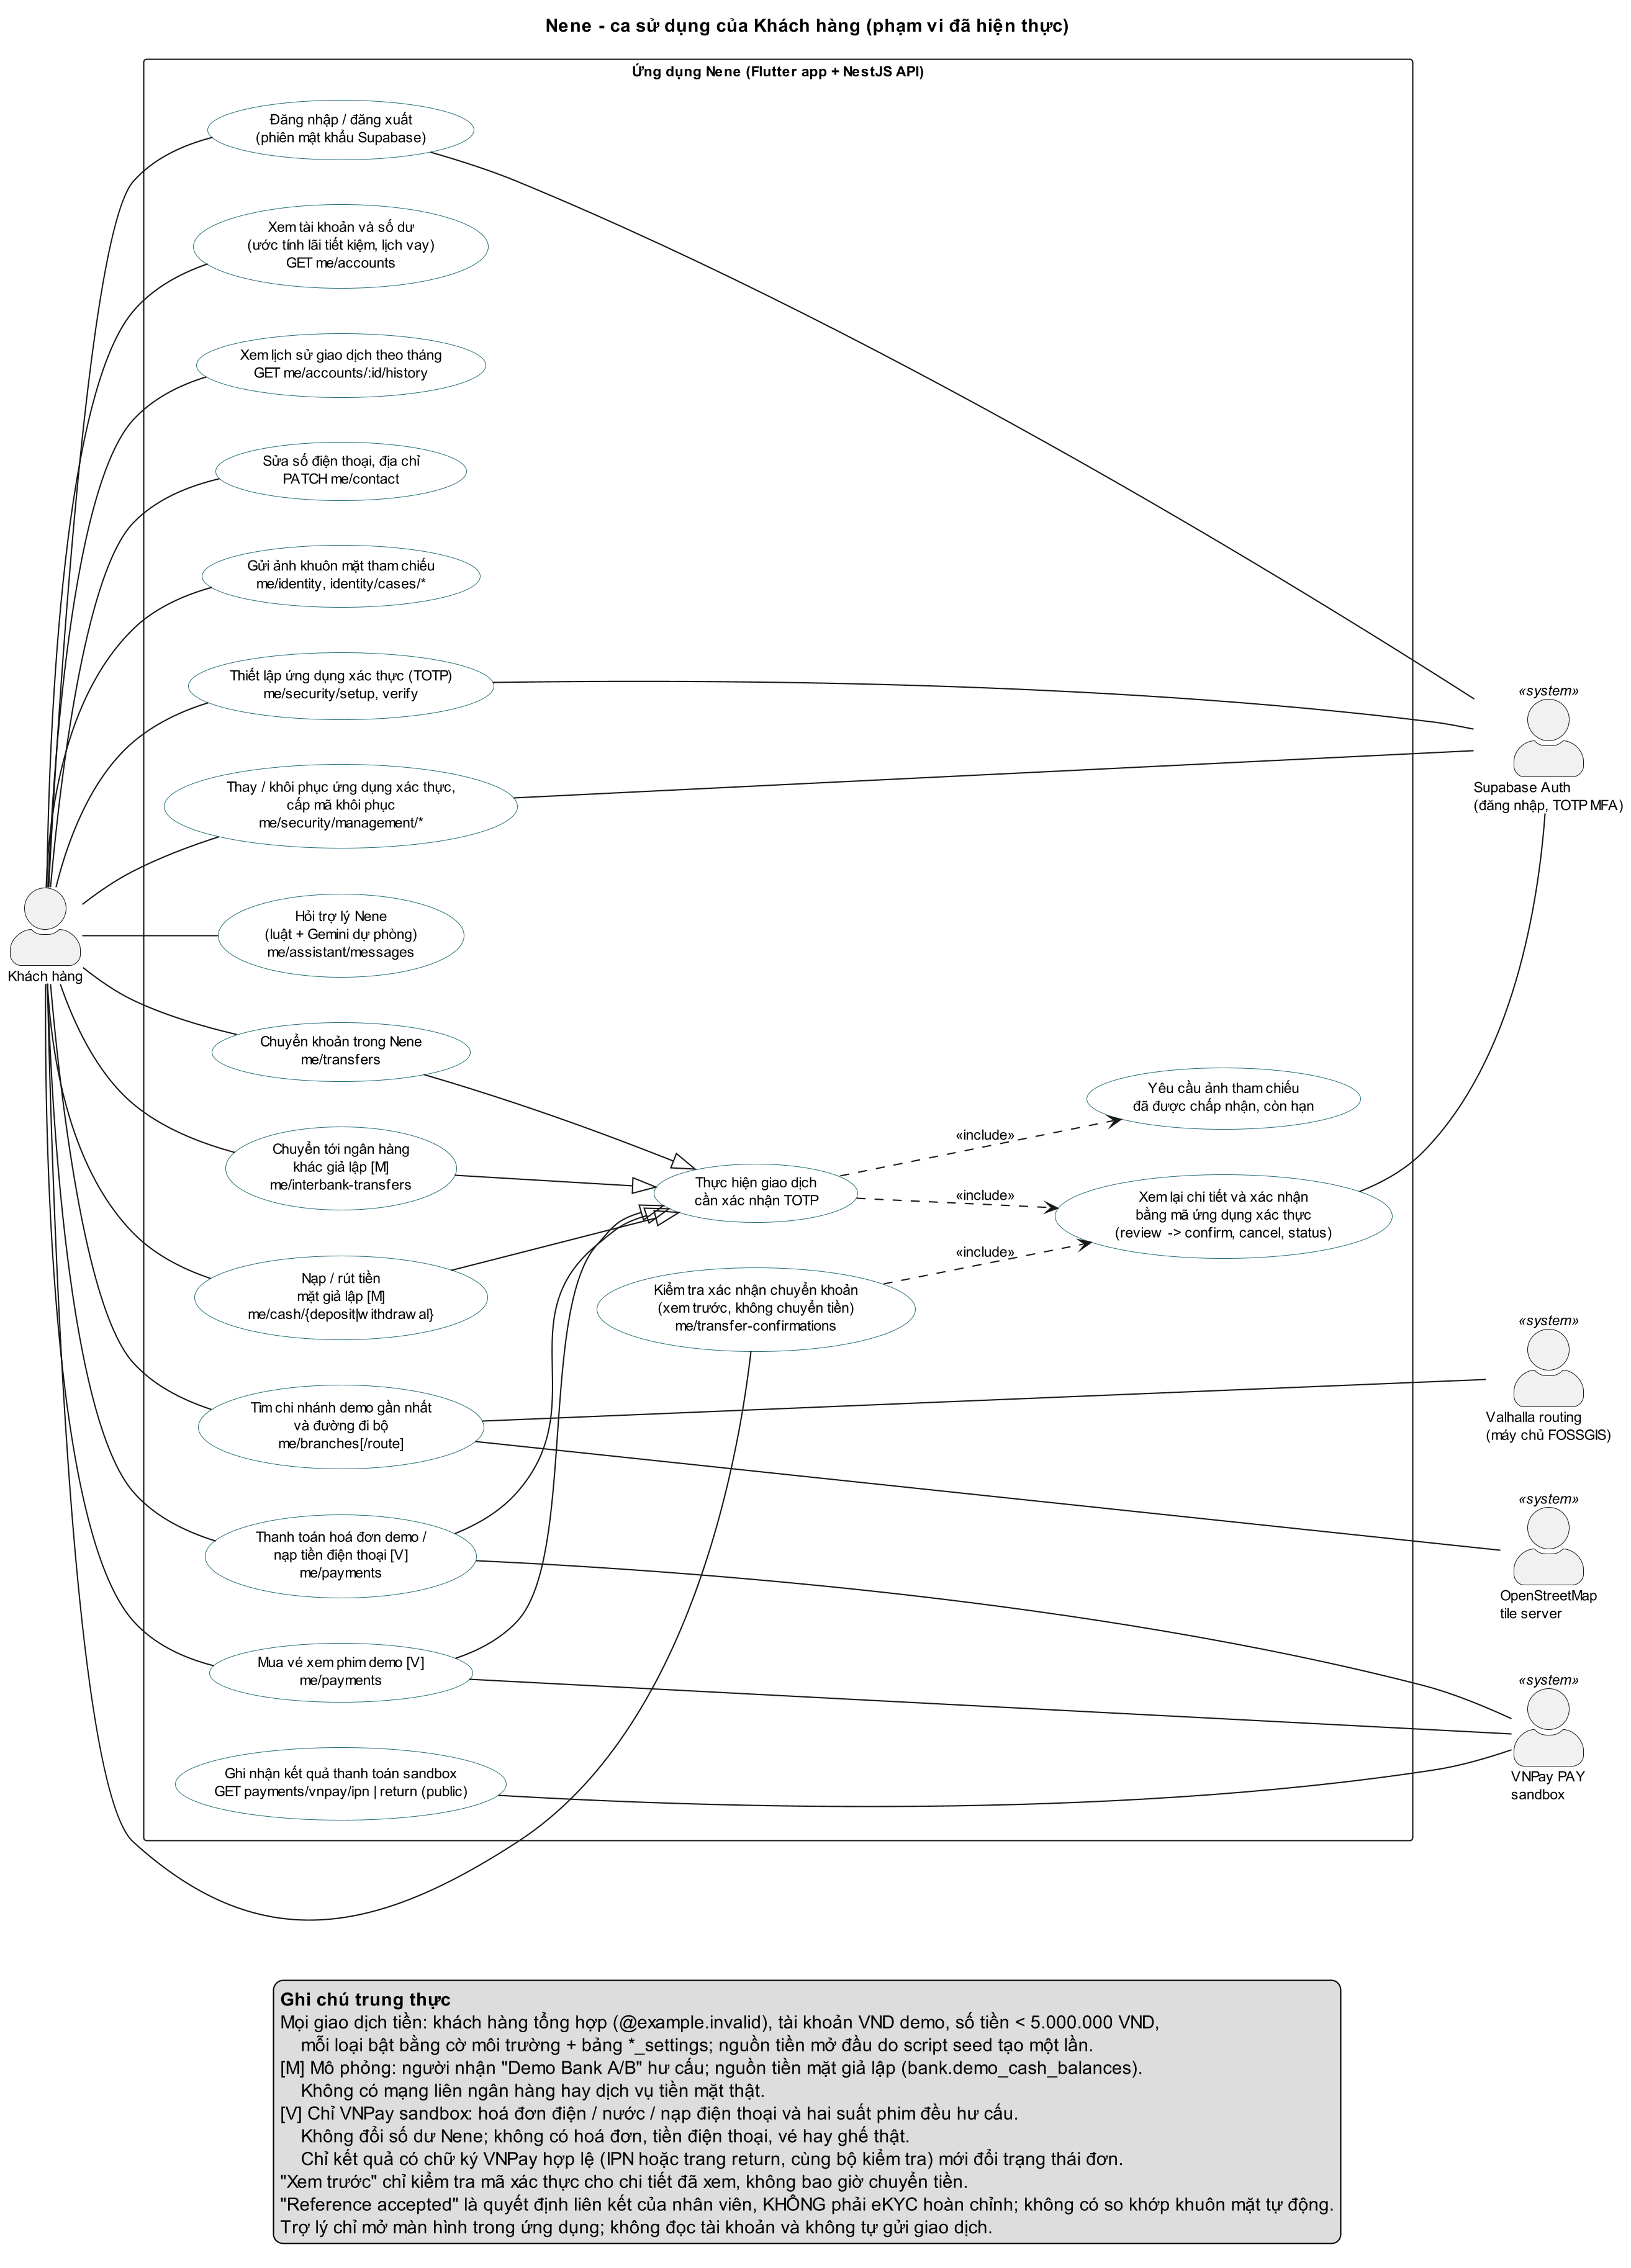
\includegraphics[width=\textwidth,height=0.8\textheight,keepaspectratio]{picture/ch2/usecase-customer}
\caption{Biểu đồ ca sử dụng của khách hàng}
\label{fig:ch2-usecase-customer}
\end{figure}

Điểm thiết kế quan trọng nhất của biểu đồ khách hàng là ca sử dụng trừu tượng \emph{Thực hiện giao dịch cần xác nhận TOTP}. Năm ca sử dụng có dịch chuyển tiền hoặc thanh toán (chuyển khoản trong Nene, chuyển khác ngân hàng mô phỏng, nạp/rút tiền mô phỏng, thanh toán hoá đơn demo, mua vé phim demo) đều là chuyên biệt hoá (generalization) của ca sử dụng này, và ca sử dụng này luôn bao gồm (\texttt{<{}<include>{}>}) hai ca sử dụng con: \emph{Xem lại chi tiết và xác nhận bằng mã ứng dụng xác thực} và \emph{Yêu cầu ảnh tham chiếu đã được chấp nhận, còn hạn}. Quan hệ này phản ánh đúng thiết kế ở backend: mọi giao dịch tiền dùng chung một quy trình xác nhận (Mục~\ref{sec:ch2-class-backend}), nên không thể có giao dịch nào bỏ qua bước 2FA. Ca sử dụng \emph{Kiểm tra xác nhận chuyển khoản} là chế độ xem trước: nó cũng đi qua bước xác nhận nhưng không bao giờ chuyển tiền. Ca sử dụng \emph{Ghi nhận kết quả thanh toán sandbox} do VNPay khởi phát chứ không phải khách hàng.

\begin{figure}[H]
\centering
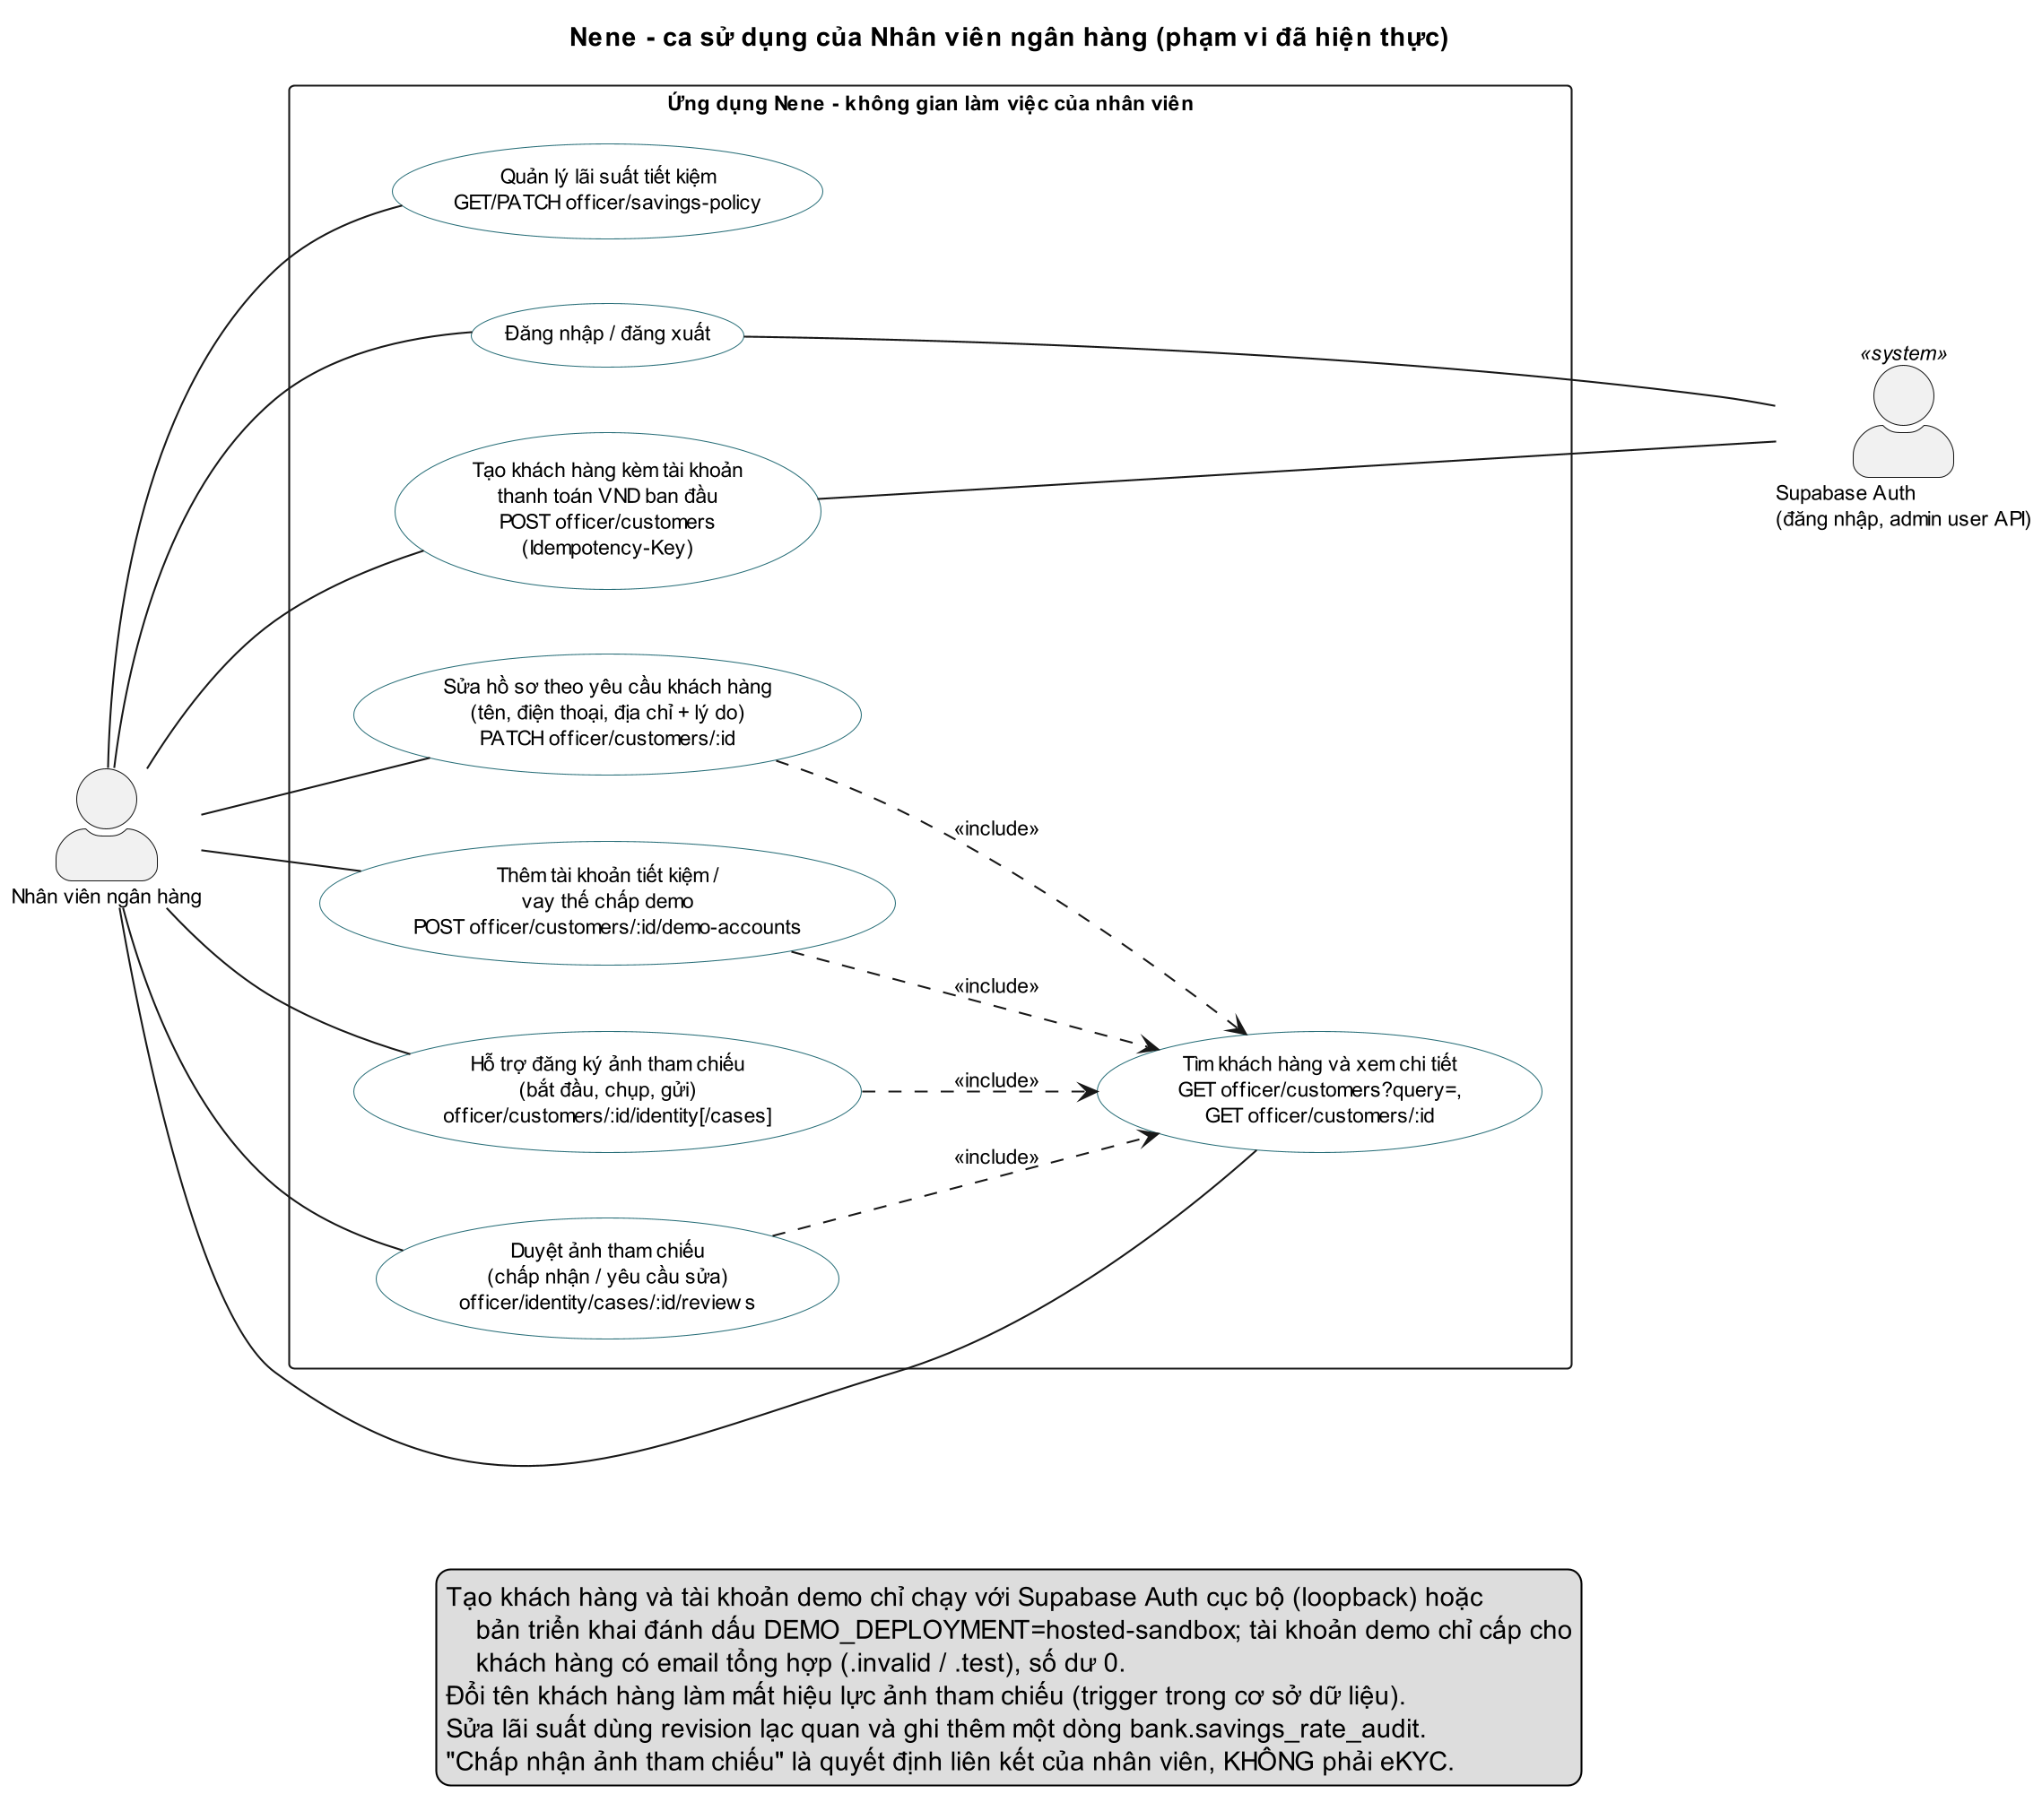
\includegraphics[width=0.95\textwidth,height=0.7\textheight,keepaspectratio]{picture/ch2/usecase-officer}
\caption{Biểu đồ ca sử dụng của nhân viên ngân hàng}
\label{fig:ch2-usecase-officer}
\end{figure}

Ở biểu đồ nhân viên, bốn ca sử dụng tác động lên một khách hàng cụ thể (sửa hồ sơ, cấp tài khoản demo, hỗ trợ đăng ký ảnh, duyệt ảnh) đều bao gồm ca sử dụng \emph{Tìm khách hàng và xem chi tiết}, vì nhân viên luôn phải chọn một khách hàng đang hoạt động trước khi thao tác. Ca sử dụng tạo khách hàng tương tác với API quản trị của Supabase Auth để tạo tài khoản đăng nhập.

\subsection{Đặc tả tóm tắt các ca sử dụng chính}
\label{sec:ch2-usecase-table}

Bảng~\ref{tab:ch2-usecases} liệt kê các ca sử dụng chính, tác nhân, mô tả ngắn và yêu cầu nghiệp vụ liên quan. Các ca sử dụng giao dịch (UC-07 đến UC-11) đều giới hạn số tiền dưới 5.000.000 VND và chỉ chạy với khách hàng tổng hợp có email đuôi \texttt{@example.\allowbreak{}invalid}.

{\small
\begin{longtable}{>{\raggedright\arraybackslash}p{0.07\textwidth}>{\raggedright\arraybackslash}p{0.18\textwidth}>{\raggedright\arraybackslash}p{0.12\textwidth}>{\raggedright\arraybackslash}p{0.40\textwidth}>{\raggedright\arraybackslash}p{0.08\textwidth}}
\caption{Danh sách ca sử dụng chính}\label{tab:ch2-usecases}\\
\toprule
\textbf{Mã} & \textbf{Ca sử dụng} & \textbf{Tác nhân} & \textbf{Mô tả ngắn} & \textbf{BR} \\
\midrule
\endfirsthead
\toprule
\textbf{Mã} & \textbf{Ca sử dụng} & \textbf{Tác nhân} & \textbf{Mô tả ngắn} & \textbf{BR} \\
\midrule
\endhead
\bottomrule
\endfoot
UC-01 & Đăng nhập, đăng xuất & Khách hàng, nhân viên, Supabase Auth & Đăng nhập bằng email và mật khẩu; ứng dụng gọi \texttt{GET me} để nhận vai trò do máy chủ quy định rồi mở không gian làm việc tương ứng. Phiên chỉ giữ trong bộ nhớ. & 01, 03 \\
UC-02 & Xem tài khoản và số dư & Khách hàng & Liệt kê tài khoản thanh toán, tiết kiệm (kèm lãi suất năm và lợi nhuận ước tính tháng) và vay thế chấp (dư nợ gốc, khoản trả hằng tháng, ngày đến hạn). & 05, 06, 07 \\
UC-03 & Xem lịch sử theo tháng & Khách hàng & Xem các bút toán đã ghi sổ của một tài khoản thuộc sở hữu, lọc theo tháng, phân trang 25 dòng. & 08 \\
UC-04 & Sửa thông tin liên hệ & Khách hàng & Sửa số điện thoại và địa chỉ; mỗi lần sửa ghi một dòng nhật ký. & 02 \\
UC-05 & Gửi ảnh tham chiếu & Khách hàng (nhân viên hỗ trợ) & Đọc thông báo, chụp ảnh khuôn mặt, lưu riêng tư và gửi duyệt. Trên Android ứng dụng kiểm tra có đúng một khuôn mặt. & 03 (một phần) \\
UC-06 & Quản lý ứng dụng xác thực & Khách hàng, Supabase Auth & Thiết lập TOTP lần đầu; thay thế, khôi phục bằng mã dự phòng, cấp mã khôi phục. & 04 \\
UC-07 & Chuyển khoản trong Nene & Khách hàng & Chuyển giữa hai tài khoản thanh toán VND; xem lại, xác nhận TOTP, ghi sổ nguyên tử, nhận biên lai. & 04, 08, 09 \\
UC-08 & Chuyển khác ngân hàng (mô phỏng) & Khách hàng & Chuyển tới người nhận hư cấu tại ``Demo Bank A/B''; không có mạng liên ngân hàng thật. & 04, 09 \\
UC-09 & Nạp, rút tiền (mô phỏng) & Khách hàng & Chuyển tiền giữa tài khoản thanh toán/tiết kiệm và nguồn tiền mặt giả lập của khách hàng. & 04, 08 \\
UC-10 & Thanh toán hoá đơn, nạp điện thoại & Khách hàng, VNPay sandbox & Hoá đơn điện, nước và nạp điện thoại hư cấu với số tiền cố định; xác nhận TOTP rồi thanh toán trên trang VNPay sandbox. & 04, 10, 11 \\
UC-11 & Mua vé xem phim & Khách hàng, VNPay sandbox & Hai suất phim hư cấu, cùng quy trình với UC-10; không phát hành vé thật. & 04, 10, 12 \\
UC-12 & Tìm chi nhánh và đường đi bộ & Khách hàng, Valhalla, OSM & Lấy vị trí một lần, hiển thị chi nhánh trong bán kính 5~km, chọn chi nhánh gần nhất và vẽ đường đi bộ ngắn nhất. & 13 \\
UC-13 & Hỏi trợ lý Nene & Khách hàng & Nhận câu hỏi tiếng Việt hoặc tiếng Anh, trả lời kèm liên kết mở đúng màn hình (lịch sử theo tháng, chuyển khoản, nạp/rút, hoá đơn, vé phim). & 14 \\
UC-14 & Tạo khách hàng & Nhân viên, Supabase Auth & Tạo tài khoản đăng nhập, hồ sơ và một tài khoản thanh toán VND số dư 0 trong một thao tác có khoá chống trùng (Idempotency-Key). & 01, 02 \\
UC-15 & Tìm, xem khách hàng & Nhân viên & Tìm theo tên, email hoặc số điện thoại (tối đa 20 kết quả); xem hồ sơ và danh sách tài khoản. & 02 \\
UC-16 & Sửa hồ sơ theo yêu cầu & Nhân viên & Sửa tên, điện thoại, địa chỉ kèm lý do yêu cầu của khách hàng; đổi tên làm mất hiệu lực ảnh tham chiếu. & 02 \\
UC-17 & Cấp tài khoản demo & Nhân viên & Thêm một tài khoản tiết kiệm hoặc vay thế chấp demo (số dư 0, lịch trả mẫu) cho khách hàng tổng hợp. & 05, 07 \\
UC-18 & Hỗ trợ và duyệt ảnh tham chiếu & Nhân viên & Hỗ trợ khách hàng chụp và gửi ảnh; xem ảnh, xác nhận liên kết với khách hàng để chấp nhận, hoặc yêu cầu chụp lại kèm lý do. & 03 (một phần) \\
UC-19 & Quản lý lãi suất tiết kiệm & Nhân viên & Đổi lãi suất năm (đơn vị điểm cơ bản) kèm lý do, kiểm tra phiên bản lạc quan, ghi nhật ký. & 06 \\
UC-20 & Ghi nhận kết quả thanh toán & VNPay sandbox & Nhận kết quả có chữ ký qua IPN hoặc trang return, kiểm tra chữ ký, mã đơn, số tiền rồi cập nhật trạng thái đơn. & 10 \\
\end{longtable}
}

\subsection{Yêu cầu phi chức năng}
\label{sec:ch2-nfr}

Bên cạnh chức năng, nhóm đặt các yêu cầu phi chức năng sau. Chúng là những quyết định của dự án (không phải quy tắc của đề bài) và là cơ sở cho các nguyên tắc thiết kế ở Mục~\ref{sec:ch2-principles}:
\begin{itemize}
  \item \textbf{Bảo mật và phân quyền}: mọi quyết định cấp quyền, quyền sở hữu tài khoản và mọi thay đổi số dư nằm ở máy chủ; ứng dụng không thể tự đặt số dư, tự cấp vai trò, tự duyệt ảnh của mình hay đặt lãi suất.
  \item \textbf{Toàn vẹn dữ liệu tài chính}: số dư, biên lai và lịch sử phải thay đổi cùng nhau hoặc không thay đổi; một yêu cầu bị gửi lặp không được trừ tiền hai lần.
  \item \textbf{Trung thực về phạm vi}: các dịch vụ mô phỏng, dữ liệu tổng hợp và môi trường sandbox phải được đánh dấu cả trong giao diện lẫn trong cơ sở dữ liệu.
  \item \textbf{Khả năng bảo trì}: cấu trúc đơn giản phù hợp nhóm 2--3 người: một ứng dụng di động, một backend, một cơ sở dữ liệu; schema được quản lý bằng migration trong mã nguồn.
  \item \textbf{Nền tảng}: Android là nền tảng nộp bài; giữ khả năng mở rộng sang iOS về sau.
\end{itemize}

% ======================================================================
\section{Kiến trúc tổng thể và lý do lựa chọn công nghệ}
\label{sec:ch2-architecture}

\subsection{Kiến trúc client--server}
\label{sec:ch2-client-server}

Nene theo kiến trúc client--server ba tầng: ứng dụng Flutter trên điện thoại (tầng trình bày), một API NestJS duy nhất (tầng nghiệp vụ) và các dịch vụ được quản lý của Supabase (tầng dữ liệu). Hình~\ref{fig:ch2-component} là sơ đồ thành phần và hạ tầng của bản demo đã triển khai.

\begin{figure}[H]
\centering
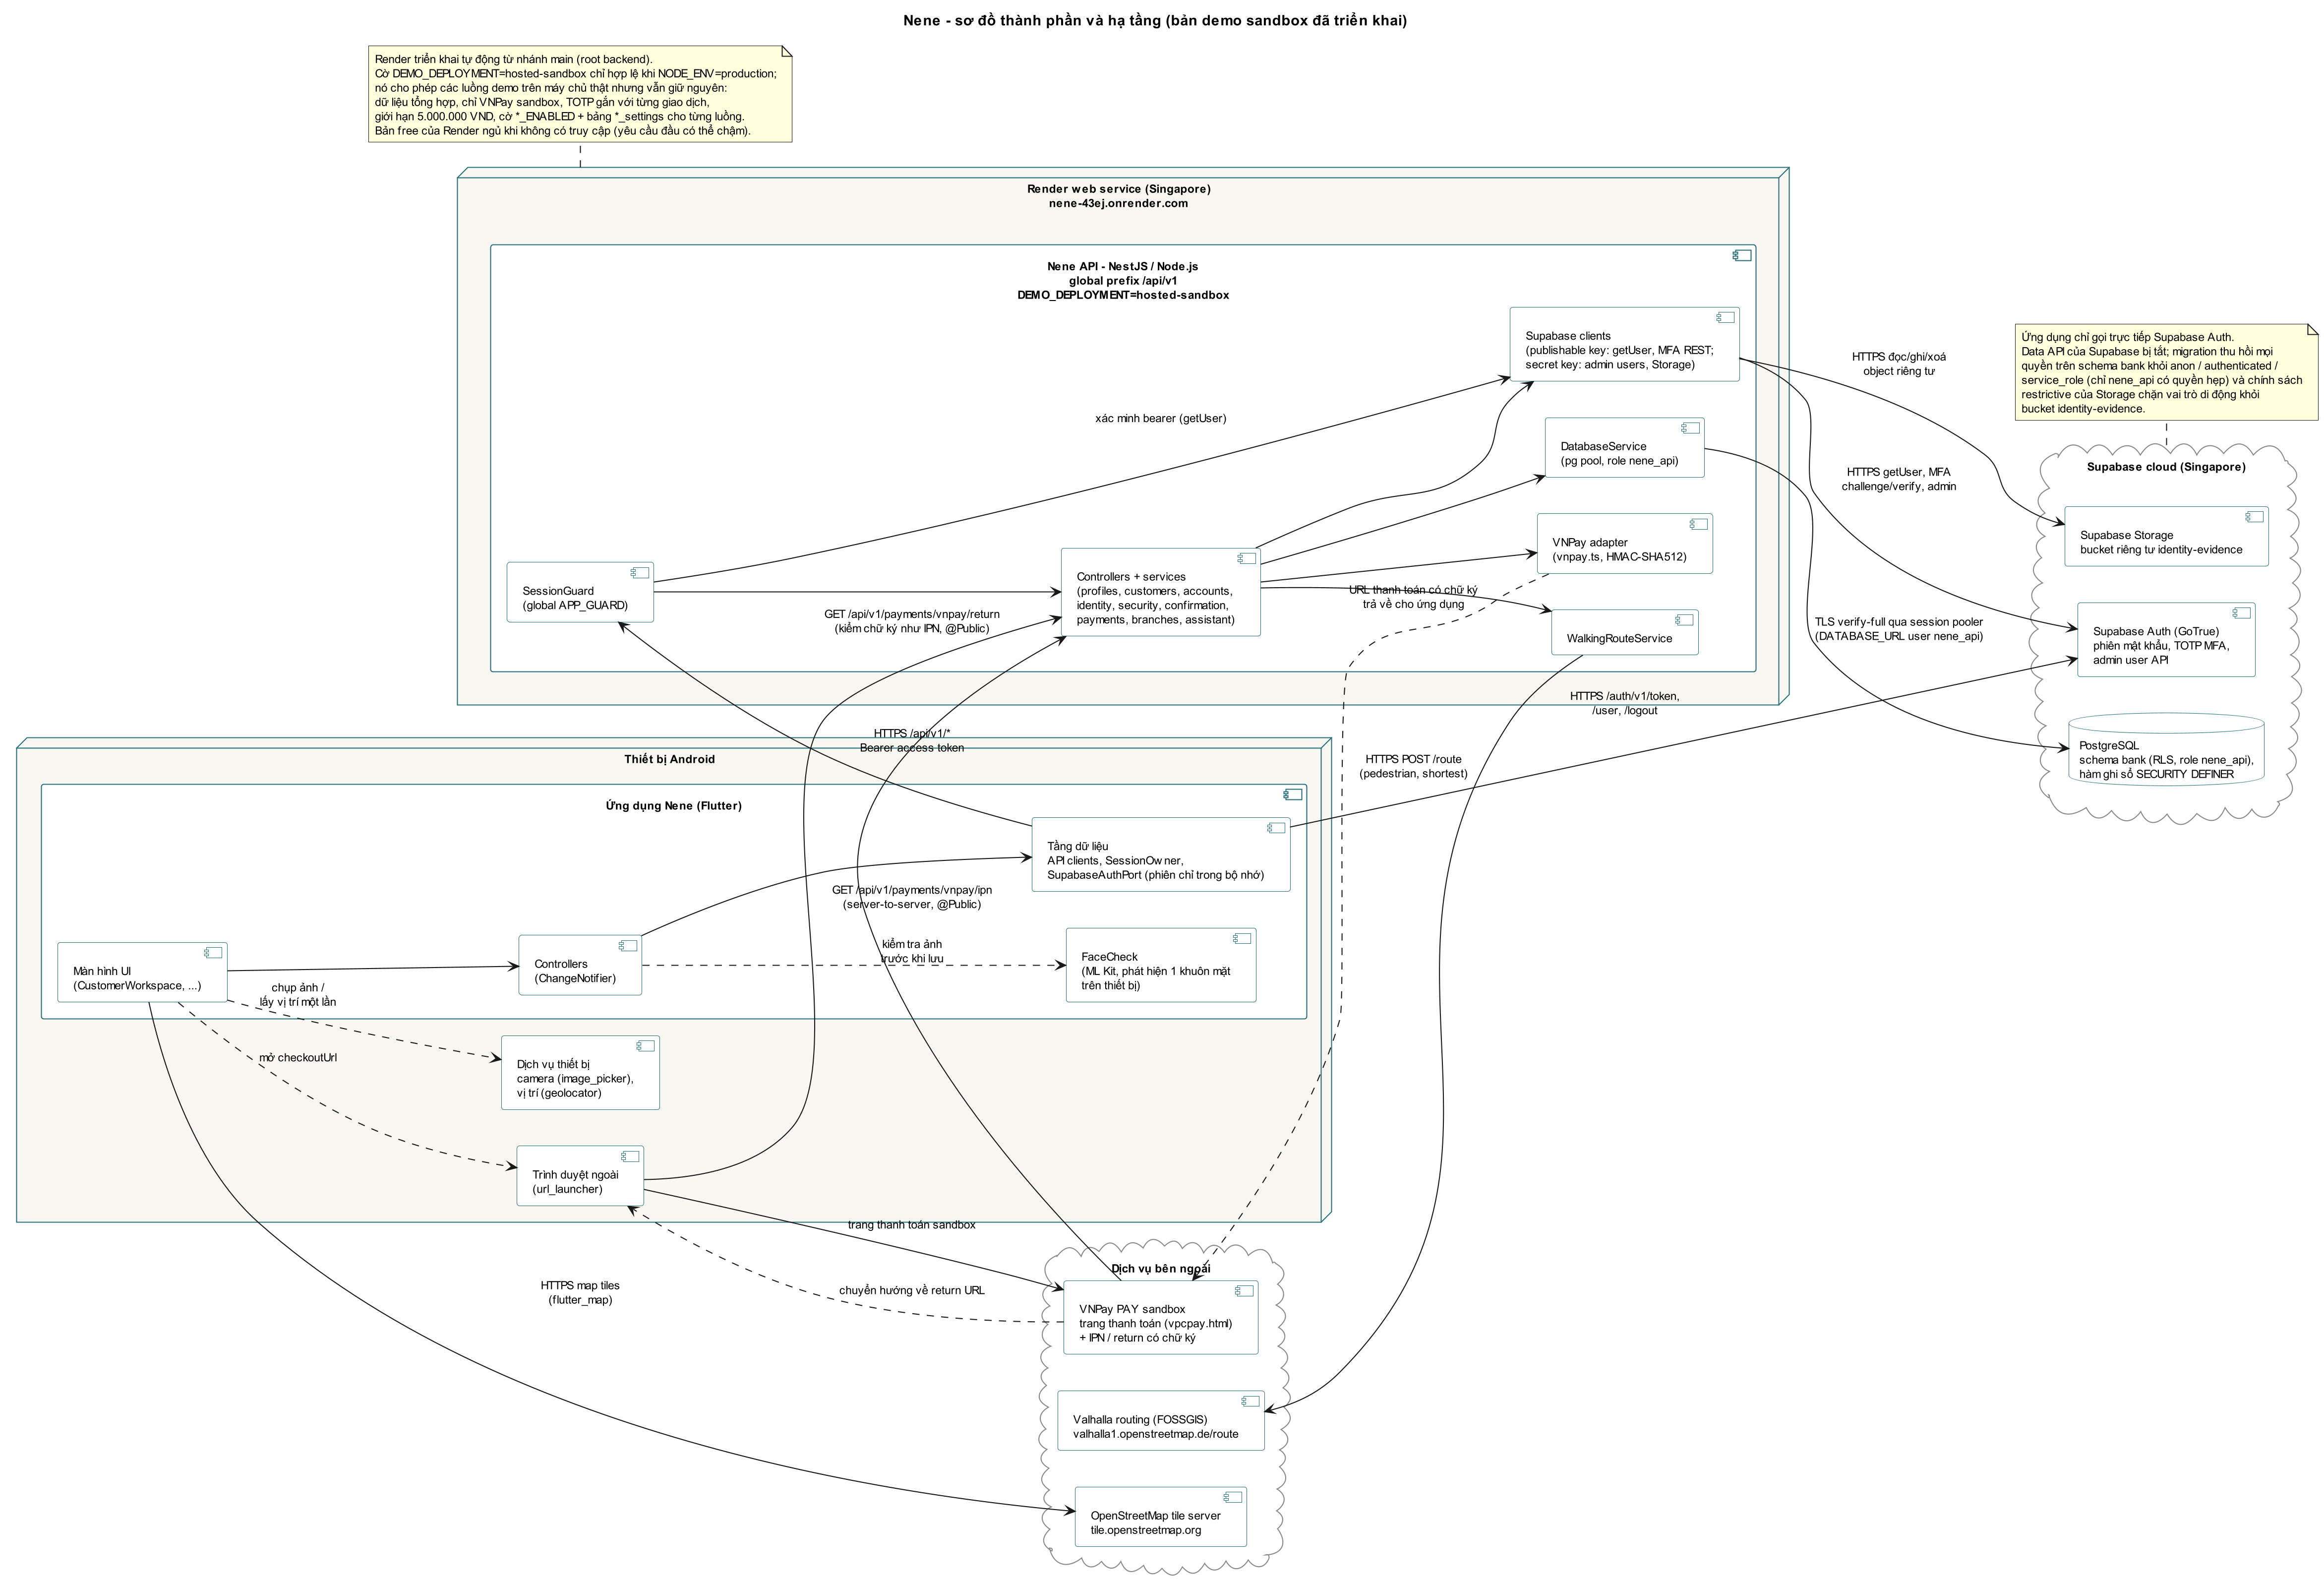
\includegraphics[angle=90,width=\textwidth,height=0.8\textheight,keepaspectratio]{picture/ch2/component}
\caption{Sơ đồ thành phần và hạ tầng triển khai của Nene}
\label{fig:ch2-component}
\end{figure}

Các luồng chính trong sơ đồ như sau:
\begin{itemize}
  \item \textbf{Ứng dụng $\rightarrow$ Supabase Auth}: ứng dụng chỉ gọi trực tiếp Supabase cho đăng nhập, làm mới và thu hồi phiên (\texttt{/\allowbreak{}auth/\allowbreak{}v1/\allowbreak{}token}, \texttt{/\allowbreak{}user}, \texttt{/\allowbreak{}logout}). Phiên nhận được chỉ giữ trong bộ nhớ.
  \item \textbf{Ứng dụng $\rightarrow$ Nene API}: mọi thao tác đọc và ghi dữ liệu ngân hàng đi qua HTTPS tới \texttt{/\allowbreak{}api/\allowbreak{}v1/\allowbreak{}*} kèm access token dạng Bearer. Ứng dụng không có quyền truy cập trực tiếp bất kỳ bảng nào.
  \item \textbf{Nene API $\rightarrow$ Supabase}: \texttt{SessionGuard} xác minh token với Supabase Auth; \texttt{Database\allowbreak{}Service} kết nối PostgreSQL bằng vai trò hạn chế \texttt{nene\_\allowbreak{}api} qua TLS với kiểm tra chứng chỉ đầy đủ (\texttt{verify-\allowbreak{}full}); ảnh tham chiếu được đọc/ghi vào bucket riêng tư bằng khoá bí mật chỉ có ở máy chủ.
  \item \textbf{Dịch vụ ngoài}: backend ký URL thanh toán VNPay sandbox và nhận kết quả có chữ ký; backend gọi Valhalla để tính đường đi bộ; ứng dụng tải ảnh nền bản đồ từ máy chủ tile của OpenStreetMap \parencite{ch2-osm-tiles}.
  \item \textbf{Dịch vụ trên thiết bị}: camera (\texttt{image\_\allowbreak{}picker}), vị trí một lần (\texttt{geolocator}), trình duyệt ngoài (\texttt{url\_\allowbreak{}launcher}) để mở trang thanh toán, và bộ phát hiện khuôn mặt ML Kit chạy hoàn toàn trên thiết bị \parencite{ch2-mlkit-face}.
\end{itemize}

Kiến trúc này cố ý tập trung toàn bộ logic nghiệp vụ vào một backend. Ứng dụng di động là môi trường không tin cậy: mã có thể bị sửa, yêu cầu có thể bị gửi trực tiếp bằng công cụ khác. Vì vậy mọi kiểm tra có ý nghĩa bảo mật (vai trò, quyền sở hữu, số dư, giới hạn, 2FA) đều được thực hiện lại ở NestJS và ở các ràng buộc của PostgreSQL, bất kể giao diện đã kiểm tra hay chưa.

\subsection{Lựa chọn công nghệ và các phương án đã cân nhắc}
\label{sec:ch2-tech}

Đề bài yêu cầu ứng dụng Android, lưu dữ liệu trong cơ sở dữ liệu (ưu tiên trên đám mây, Firebase được nêu như một ví dụ), eKYC, 2FA và phát hành trên Google Play; đề bài không bắt buộc framework, ngôn ngữ backend hay hệ quản trị cơ sở dữ liệu cụ thể. Bộ công nghệ Flutter/Dart + NestJS/TypeScript + Supabase được nhóm chốt ngày 13/10/2026, thay cho đề xuất ban đầu dùng Kotlin/Jetpack Compose và Firebase. Bảng~\ref{tab:ch2-tech} tóm tắt lựa chọn, lý do và phương án thay thế đã cân nhắc.

{\small
\begin{longtable}{>{\raggedright\arraybackslash}p{0.14\textwidth}>{\raggedright\arraybackslash}p{0.16\textwidth}>{\raggedright\arraybackslash}p{0.36\textwidth}>{\raggedright\arraybackslash}p{0.22\textwidth}}
\caption{Lựa chọn công nghệ và lý do}\label{tab:ch2-tech}\\
\toprule
\textbf{Thành phần} & \textbf{Lựa chọn} & \textbf{Lý do} & \textbf{Phương án đã cân nhắc} \\
\midrule
\endfirsthead
\toprule
\textbf{Thành phần} & \textbf{Lựa chọn} & \textbf{Lý do} & \textbf{Phương án đã cân nhắc} \\
\midrule
\endhead
\bottomrule
\endfoot
Ứng dụng di động & Flutter 3.47 / Dart 3.13 & Một mã nguồn cho cả hai vai trò và nhiều màn hình; Android là nền tảng nộp bài, giữ khả năng build iOS về sau; có sẵn các plugin camera, vị trí, bản đồ, ML Kit. & Kotlin + Jetpack Compose (chỉ Android); React Native. \\
Quản lý trạng thái & \texttt{Change\allowbreak{}Notifier} có sẵn của Flutter & Đủ cho các luồng hiện có, không thêm thư viện bên ngoài; dễ kiểm thử \parencite{ch2-flutter-state}. & Provider, Riverpod, BLoC. \\
Backend & NestJS 12 / TypeScript 6 trên Node.js 24 & Cấu trúc module, controller, provider; tiêm phụ thuộc (DI) và guard có sẵn; gom phân quyền, quy tắc tài chính, callback thanh toán vào một nơi \parencite{ch2-nestjs-providers,ch2-nestjs-guards}. & Supabase Edge Functions; cho ứng dụng truy cập thẳng cơ sở dữ liệu. \\
Truy cập dữ liệu & Thư viện \texttt{pg} với SQL tham số hoá, migration SQL & Kiểm soát chính xác giao dịch, khoá dòng (\texttt{FOR UPDATE}) và câu lệnh; không có tầng ORM che khuất hành vi khoá. & ORM như Prisma hoặc TypeORM. \\
Cơ sở dữ liệu & PostgreSQL trên Supabase (Singapore) & Quan hệ rõ ràng giữa khách hàng, tài khoản, giao dịch; khoá ngoại và \texttt{CHECK}; giao dịch ACID nhiều bảng; hàm PL/pgSQL; phân quyền theo cột và bảo mật mức dòng (RLS). & Cloud Firestore (Firebase), SQLite trên thiết bị. \\
Xác thực & Supabase Auth & Đăng nhập mật khẩu, quản lý phiên, MFA TOTP theo RFC~6238 có sẵn \parencite{ch2-supabase-auth,ch2-supabase-mfa,ch2-rfc6238}. & Firebase Authentication; tự xây dịch vụ xác thực. \\
Lưu trữ ảnh & Supabase Storage (bucket riêng tư) & Ảnh tham chiếu không bao giờ công khai; chỉ backend đọc/ghi \parencite{ch2-supabase-storage}. & Lưu ảnh trong bảng cơ sở dữ liệu. \\
Thanh toán & VNPay PAY sandbox & Cổng thanh toán Việt Nam được đề bài gợi ý; có sandbox và chữ ký HMAC-SHA512 \parencite{ch2-vnpay-pay}. & Stripe (test mode). \\
Bản đồ, tìm đường & \texttt{flutter\_\allowbreak{}map} + tile OpenStreetMap; Valhalla (FOSSGIS) & Miễn phí, không cần khoá API hay tài khoản thanh toán; Valhalla hỗ trợ đi bộ (\texttt{pedestrian}) với tuỳ chọn quãng đường ngắn nhất \parencite{ch2-valhalla}. & Google Maps Platform (cần khoá API và tài khoản thanh toán). \\
Phát hiện khuôn mặt & Google ML Kit (mô hình đóng gói trong APK) & Chạy trên thiết bị, không gửi ảnh đi, không cần tài khoản. & Dịch vụ eKYC thương mại; AWS (chưa quyết định). \\
Lưu trữ API & Render web service (Singapore) & Triển khai từ GitHub, cùng khu vực với Supabase, có gói miễn phí. & Tự quản máy chủ ảo. \\
\end{longtable}
}

\paragraph{Supabase/PostgreSQL thay cho Firebase.} Đề bài nêu Firebase như một ví dụ. Cloud Firestore là cơ sở dữ liệu tài liệu (NoSQL) \parencite{ch2-firestore}; nó có giao dịch và quy tắc bảo mật, nhưng các ràng buộc quan hệ như khoá ngoại hay \texttt{CHECK} trên số tiền phải tự kiểm tra trong mã hoặc trong quy tắc bảo mật. Dữ liệu ngân hàng có quan hệ chặt chẽ: một khách hàng có nhiều tài khoản, một giao dịch chạm tới hai tài khoản, một biên lai phải gắn với đúng một lần xác nhận. PostgreSQL cho phép diễn đạt các bất biến này ngay trong schema (khoá ngoại \texttt{ON DELETE RESTRICT}, \texttt{balance\_\allowbreak{}minor >= 0}, số tiền nằm trong khoảng cho phép), cập nhật nhiều bảng trong một giao dịch ACID với khoá dòng tường minh \parencite{ch2-pg-transactions,ch2-pg-locking}, và giới hạn quyền đến từng cột kết hợp bảo mật mức dòng \parencite{ch2-pg-rls}. Đồng thời Supabase vẫn đáp ứng tiêu chí ``cơ sở dữ liệu trên dịch vụ đám mây'' của TR-03 và cung cấp sẵn xác thực và lưu trữ tệp, giúp giảm khối lượng hạ tầng phải tự vận hành. Đổi lại, nhóm phải tự viết migration và tự xử lý tranh chấp đồng thời.

\paragraph{Flutter cho Android trước, iOS sau.} Một mã nguồn Dart phục vụ hai vai trò và mười bảy trang trong không gian làm việc. Bản nộp là Android; bản iOS đòi hỏi macOS và Xcode nên chưa được build hay kiểm thử. Flutter cũng chạy được trên trình duyệt, nhóm tận dụng điều này để xem trước giao diện khi phát triển (bộ phát hiện khuôn mặt không có trên web và được thay bằng một bản cài đặt ``không khả dụng'').

\paragraph{Một backend NestJS thay vì để ứng dụng truy cập thẳng dữ liệu.} Supabase cho phép ứng dụng truy vấn bảng trực tiếp qua Data API, nhưng khi đó mọi quy tắc nghiệp vụ phải nằm trong chính sách RLS và ứng dụng sẽ chạm vào dữ liệu tài chính. Nhóm chọn một backend duy nhất để gom phân quyền, xác nhận giao dịch, tích hợp VNPay và tìm đường vào mã TypeScript có kiểu, có thể kiểm thử đơn vị; NestJS cung cấp sẵn cơ chế module, tiêm phụ thuộc và guard. Không dùng thêm Edge Functions để tránh hai nơi chứa logic. Cái giá là thêm một dịch vụ phải triển khai và vận hành.

Bảng~\ref{tab:ch2-versions} liệt kê phiên bản các thư viện chính được khoá trong \texttt{app/\allowbreak{}pubspec.\allowbreak{}yaml} và \texttt{backend/\allowbreak{}package.\allowbreak{}json}.

\begin{table}[H]
\centering
\small
\caption{Phiên bản các thư viện chính}
\label{tab:ch2-versions}
\begin{tabularx}{\textwidth}{>{\raggedright\arraybackslash}p{0.38\textwidth}X}
\toprule
\textbf{Thư viện} & \textbf{Vai trò} \\
\midrule
\texttt{@nestjs/\allowbreak{}common}, \texttt{core} 12.1.3 & Framework backend \\
\texttt{pg} 8.23.1 & Driver PostgreSQL, SQL tham số hoá \\
\texttt{@supabase/\allowbreak{}supabase-\allowbreak{}js} 2.117.3 & Xác minh phiên, API quản trị, Storage (phía máy chủ) \\
\texttt{sharp} 0.35.5 & Giải mã và mã hoá lại ảnh tham chiếu \\
\texttt{http} 1.6.0 & Gọi API từ ứng dụng \\
\texttt{flutter\_\allowbreak{}map} 8.3.2, \texttt{latlong2} 0.9.1 & Bản đồ và toạ độ \\
\texttt{geolocator} 14.1.2 & Lấy vị trí một lần \\
\texttt{image\_\allowbreak{}picker} 1.2.4 & Chụp ảnh tham chiếu \\
\texttt{url\_\allowbreak{}launcher} 6.3.3 & Mở trang thanh toán VNPay \\
\texttt{google\_\allowbreak{}mlkit\_\allowbreak{}face\_\allowbreak{}detection} 1.0.3 & Phát hiện khuôn mặt trên thiết bị \\
\bottomrule
\end{tabularx}
\end{table}

\subsection{Hạ tầng triển khai}
\label{sec:ch2-deployment}

Bản demo được triển khai như sau (Hình~\ref{fig:ch2-component}):
\begin{itemize}
  \item \textbf{API}: một Render web service ở Singapore (\texttt{https:/\allowbreak{}/\allowbreak{}nene-\allowbreak{}43ej.\allowbreak{}onrender.\allowbreak{}com}) build từ thư mục \texttt{backend} của nhánh \texttt{main}, kiểm tra sức khoẻ qua \texttt{/\allowbreak{}api/\allowbreak{}v1/\allowbreak{}health} \parencite{ch2-render}. Gói miễn phí ngủ khi không có truy cập nên yêu cầu đầu tiên có thể mất khoảng một phút.
  \item \textbf{Dữ liệu}: một dự án Supabase cloud ở Singapore. Cả 17 migration đã được áp dụng; Data API của Supabase bị tắt nên các bảng ngân hàng chỉ truy cập được qua NestJS. API kết nối qua session pooler bằng tài khoản \texttt{nene\_\allowbreak{}api} và chứng chỉ gốc của Supabase được đóng gói trong mã nguồn để kiểm tra TLS đầy đủ.
  \item \textbf{Ứng dụng}: gói \texttt{vn.\allowbreak{}nene.\allowbreak{}bank} phiên bản 1.0.1 (AAB ký bằng upload key) trên kênh kiểm thử nội bộ của Google Play.
  \item \textbf{Phát triển cục bộ}: Supabase chạy bằng Docker với các cổng chỉ gắn vào loopback; API NestJS chạy cục bộ.
\end{itemize}

Cấu hình được đọc và kiểm tra ngay khi khởi động (\texttt{backend/\allowbreak{}src/\allowbreak{}config/\allowbreak{}environment.\allowbreak{}ts}); cấu hình sai làm ứng dụng dừng thay vì chạy ở trạng thái không an toàn (\emph{fail closed}). Các luồng demo (tạo khách hàng, tài khoản demo, chuyển khoản, tiền mặt mô phỏng, liên ngân hàng mô phỏng, VNPay sandbox, tìm đường) chỉ được bật khi Auth và cơ sở dữ liệu ở loopback và không phải production, hoặc khi bản triển khai được đánh dấu tường minh \texttt{DEMO\_\allowbreak{}DEPLOYMENT=hosted-\allowbreak{}sandbox}; dấu này chỉ hợp lệ cùng \texttt{NODE\_\allowbreak{}ENV=production}. Dấu này không nới lỏng bất kỳ kiểm tra nào: vẫn chỉ dữ liệu tổng hợp, chỉ VNPay sandbox, TOTP gắn với từng giao dịch, giới hạn 5.000.000 VND, và mỗi luồng tiền còn cần cờ \texttt{*\_\allowbreak{}ENABLED} riêng cùng bảng cấu hình \texttt{*\_\allowbreak{}settings} trong cơ sở dữ liệu.

% ======================================================================
\section{Nguyên tắc, mẫu thiết kế và thực hành áp dụng}
\label{sec:ch2-principles}

\subsection{Kiến trúc phân tầng}
\label{sec:ch2-layers}

Cả hai phía đều được tổ chức thành các tầng chỉ phụ thuộc theo một chiều:
\begin{itemize}
  \item \textbf{Backend}: Controller (nhận HTTP, kiểm tra hình dạng dữ liệu đầu vào) $\rightarrow$ Service (quy tắc nghiệp vụ, phân quyền, điều phối giao dịch) $\rightarrow$ \texttt{Database\allowbreak{}Service} (bao bọc \texttt{pg.\allowbreak{}Pool}) $\rightarrow$ PostgreSQL (ràng buộc, RLS, hàm ghi sổ). Bên ngoài được gói trong các lớp riêng: \texttt{Supabase\allowbreak{}Auth\allowbreak{}Service}, \texttt{Supabase\allowbreak{}Admin\allowbreak{}Service}, \texttt{Identity\allowbreak{}Storage\allowbreak{}Service}, \texttt{Walking\allowbreak{}Route\allowbreak{}Service} và module \texttt{vnpay.\allowbreak{}ts}.
  \item \textbf{Ứng dụng}: Widget giao diện $\rightarrow$ Controller (\texttt{Change\allowbreak{}Notifier}) $\rightarrow$ Repository/API client $\rightarrow$ Nene API hoặc Supabase Auth. Widget không tự dựng yêu cầu HTTP; đây cũng là kiến trúc được khuyến nghị trong tài liệu Flutter \parencite{ch2-flutter-architecture}. Các màn hình có trạng thái đơn giản (lịch sử, bản đồ chi nhánh, lãi suất, tài khoản demo) không có controller riêng mà gọi thẳng API client thông qua \texttt{Session\allowbreak{}Controller.\allowbreak{}authorized()}.
\end{itemize}
Một số controller chỉ đọc hoặc ghi rất đơn giản (\texttt{Account\allowbreak{}History\allowbreak{}Controller}, \texttt{Savings\allowbreak{}Policy\allowbreak{}Controller}, \texttt{Demo\allowbreak{}Account\allowbreak{}Controller}, \texttt{Branches\allowbreak{}Controller}) gọi thẳng \texttt{Database\allowbreak{}Service} mà không qua một lớp service riêng; nhóm chấp nhận sự giản lược này vì logic của chúng chỉ gồm một truy vấn hoặc một giao dịch ngắn, và đánh dấu rõ trên biểu đồ lớp.

\subsection{Controller--Service và tiêm phụ thuộc}
\label{sec:ch2-di}

NestJS quản lý vòng đời đối tượng qua một IoC container \parencite{ch2-fowler-di,ch2-nestjs-providers}. \texttt{AppModule} (\texttt{backend/\allowbreak{}src/\allowbreak{}app.\allowbreak{}module.\allowbreak{}ts}) đăng ký 17 controller và 12 provider; \texttt{ConfigModule} là module toàn cục cung cấp đối tượng cấu hình qua token \texttt{ENVIRONMENT}. Các lớp nhận phụ thuộc qua constructor, ví dụ \texttt{PaymentsService(db: DatabaseService,\allowbreak{} security: SecurityService,\allowbreak{} @Inject(ENVIRONMENT) env)}. Nhờ vậy khi kiểm thử có thể thay \texttt{Database\allowbreak{}Service} hoặc dịch vụ Supabase bằng bản giả. \texttt{SessionGuard} được đăng ký là \texttt{APP\_\allowbreak{}GUARD} toàn cục nên \emph{mặc định mọi route đều cần đăng nhập}; route công khai phải gắn tường minh decorator \texttt{@Public()} (chỉ có \texttt{health} và hai callback VNPay). Listing~\ref{lst:ch2-guard} trích phần chính của guard.

\begin{lstlisting}[caption={Trích \texttt{backend/\allowbreak{}src/\allowbreak{}auth/\allowbreak{}session.\allowbreak{}guard.\allowbreak{}ts}: xác minh phiên và nạp vai trò từ cơ sở dữ liệu},label={lst:ch2-guard}]
if (this.reflector.getAllAndOverride<boolean>(PUBLIC_ROUTE, [
      context.getHandler(), context.getClass()]))
  return true;
...
if (!token) throw new UnauthorizedException('A bearer session is required.');
const identity = await this.auth.verifyAccessToken(token);
const profile = await this.profiles.findById(identity.id);
if (!profile || profile.status !== 'active' ||
    !['customer', 'officer'].includes(profile.role)) {
  throw new ForbiddenException('An active application profile is required.');
}
request.user = { id: identity.id, email: identity.email,
  displayName: profile.display_name, role: profile.role,
  phone: profile.phone, address: profile.address };
\end{lstlisting}

Điểm quan trọng là vai trò được đọc từ bảng \texttt{bank.\allowbreak{}user\_\allowbreak{}profiles} theo định danh đã xác minh, không lấy từ metadata trong token mà người dùng có thể tác động. Mỗi service sau đó kiểm tra lại vai trò phù hợp (ví dụ \texttt{Customers\allowbreak{}Service.\allowbreak{}officer()} hoặc \texttt{Security\allowbreak{}Service.\allowbreak{}identity()} chỉ cho khách hàng).

\subsection{Repository và Observer trong ứng dụng Flutter}
\label{sec:ch2-repository-observer}

\textbf{Mẫu Repository} \parencite{ch2-fowler-peaa} tách nguồn dữ liệu khỏi phần còn lại của ứng dụng: các giao diện trừu tượng \texttt{Auth\allowbreak{}Repository}, \texttt{Profile\allowbreak{}Repository}, \texttt{Banking\allowbreak{}Repository}, \texttt{Identity\allowbreak{}Repository} cùng các cổng \texttt{AuthPort}, \texttt{Reference\allowbreak{}Photo\allowbreak{}Source}, \texttt{Branch\allowbreak{}Location}, \texttt{FaceCheck} được cài đặt bởi các lớp cụ thể (\texttt{Owned\allowbreak{}Auth\allowbreak{}Repository}, \texttt{ProfileApi}, \texttt{BankingApi}, \texttt{IdentityApi}, \texttt{Supabase\allowbreak{}Auth\allowbreak{}Port}, \texttt{Device\allowbreak{}Reference\allowbreak{}Photo\allowbreak{}Source}, \texttt{Device\allowbreak{}Branch\allowbreak{}Location}, \texttt{Ml\allowbreak{}Kit\allowbreak{}Face\allowbreak{}Check}). \texttt{main.\allowbreak{}dart} đóng vai trò \emph{composition root}: nó dựng các đối tượng cụ thể và truyền xuống \texttt{NeneApp}. Trong kiểm thử, các giao diện này được thay bằng bản giả nên controller và widget có thể kiểm thử mà không cần mạng, camera hay GPS.

\textbf{Mẫu Observer} \parencite{ch2-gof} được hiện thực bằng \texttt{Change\allowbreak{}Notifier}: \texttt{Session\allowbreak{}Controller}, \texttt{Customer\allowbreak{}Flow\allowbreak{}Controller}, \texttt{Identity\allowbreak{}Controller} và \texttt{Assistant\allowbreak{}Controller} giữ trạng thái và gọi \texttt{notify\allowbreak{}Listeners()} khi trạng thái đổi; widget lắng nghe và dựng lại. Ví dụ \texttt{NeneApp} lắng nghe \texttt{Session\allowbreak{}Controller.\allowbreak{}status} để chuyển giữa màn hình đăng nhập và không gian làm việc. Các lời gọi API thông thường đi qua \texttt{Session\allowbreak{}Controller.\allowbreak{}authorized(operation, role)}: hàm này chụp lại phiên trước khi gọi, từ chối nếu vai trò hiện tại không khớp, và loại bỏ kết quả nếu phiên đã thay đổi trong lúc chờ (đăng xuất, đổi người dùng), để kết quả của phiên cũ không lọt vào giao diện của phiên mới. Các API có thể làm đổi phiên (\texttt{SecurityApi}, \texttt{Confirmation\allowbreak{}Api}, \texttt{PaymentsApi}) đi qua \texttt{SessionOwner} (Mục~\ref{sec:ch2-session}).

\subsection{Máy chủ là nguồn sự thật cho mọi ghi tài chính}
\label{sec:ch2-authoritative}

Ứng dụng chỉ gửi \emph{ý định} (tài khoản nguồn, số tài khoản đích, số tiền); máy chủ quyết định mọi thứ còn lại. Nguyên tắc này được thực thi ở ba lớp:
\begin{enumerate}
  \item \textbf{API}: không có endpoint nào nhận số dư, vai trò, lãi suất do khách hàng đặt hay kết quả duyệt ảnh do khách hàng tự gửi. Đầu vào được kiểm tra chặt chẽ (chỉ chấp nhận đúng các khoá mong đợi, kiểu và độ dài hợp lệ).
  \item \textbf{Quyền cơ sở dữ liệu}: vai trò \texttt{nene\_\allowbreak{}api} \emph{không có quyền} \texttt{UPDATE} trên cột \texttt{balance\_\allowbreak{}minor} hay bất kỳ bảng biên lai nào. Từ phía API, số dư chỉ có thể thay đổi bên trong ba hàm ghi sổ (Mục~\ref{sec:ch2-atomic}); khoản tiền mở đầu tổng hợp được quản trị viên tạo một lần bằng script seed, không qua API.
  \item \textbf{Ràng buộc dữ liệu}: \texttt{CHECK} đảm bảo số dư không âm, số tiền dương và nhỏ hơn 5.000.000, đơn vị tiền là VND; chính sách RLS khi tạo tài khoản bắt buộc số dư ban đầu bằng 0.
\end{enumerate}

\subsection{Nguyên tắc đặc quyền tối thiểu với vai trò \texttt{nene\_\allowbreak{}api}}
\label{sec:ch2-least-privilege}

Backend không kết nối bằng tài khoản quản trị \texttt{postgres} mà bằng vai trò riêng \texttt{nene\_\allowbreak{}api}, được tạo trong migration đầu tiên với các thuộc tính hạn chế nhất (Listing~\ref{lst:ch2-role}). Mọi quyền trên schema \texttt{bank} bị thu hồi khỏi \texttt{public}, \texttt{anon}, \texttt{authenticated} và cả \texttt{service\_\allowbreak{}role} của Supabase; mỗi migration sau đó cấp quyền tường minh cho \texttt{nene\_\allowbreak{}api}, nhiều chỗ chỉ đến mức cột.

\begin{lstlisting}[language=SQL,caption={Trích migration \texttt{20261015000100} và \texttt{20261020000100}: vai trò hạn chế và quyền theo cột},label={lst:ch2-role}]
create role nene_api
  nologin nosuperuser nocreatedb nocreaterole noinherit noreplication nobypassrls;
revoke all on schema bank from public, anon, authenticated, service_role;
grant usage on schema bank to nene_api;
...
grant insert (id, owner_id, type, currency) on bank.banking_accounts to nene_api;
create policy api_create_accounts on bank.banking_accounts for insert to nene_api with check (
  balance_minor = 0 and status = 'active' and exists (
    select 1 from bank.user_profiles where id = owner_id and role = 'customer' and status = 'active'
  )
);
\end{lstlisting}

Ví dụ trên cho thấy \texttt{nene\_\allowbreak{}api} chỉ được chèn bốn cột của tài khoản; cột \texttt{balance\_\allowbreak{}minor} lấy giá trị mặc định 0 và chính sách RLS từ chối mọi tài khoản mới không phải số dư 0 hoặc không thuộc một khách hàng đang hoạt động. Tương tự, \texttt{nene\_\allowbreak{}api} chỉ được sửa \texttt{display\_\allowbreak{}name}, \texttt{phone}, \texttt{address}, \texttt{updated\_\allowbreak{}at} của hồ sơ, không sửa được \texttt{role} hay \texttt{status}. Trên môi trường cloud, vai trò này được bật đăng nhập bằng một mật khẩu riêng khác mật khẩu quản trị.

\subsection{Ghi sổ nguyên tử bằng hàm \texttt{SECURITY DEFINER}}
\label{sec:ch2-atomic}

Ba hàm PL/pgSQL \texttt{bank.\allowbreak{}post\_\allowbreak{}local\_\allowbreak{}transfer}, \texttt{bank.\allowbreak{}post\_\allowbreak{}local\_\allowbreak{}cash} và \texttt{bank.\allowbreak{}post\_\allowbreak{}local\_\allowbreak{}interbank} là con đường duy nhất làm thay đổi số dư. Chúng được khai báo \texttt{SECURITY DEFINER} (chạy với quyền của chủ sở hữu hàm) và cố định \texttt{search\_\allowbreak{}path=pg\_\allowbreak{}catalog} để tránh bị chiếm quyền qua đối tượng trùng tên \parencite{ch2-pg-create-function}; \texttt{nene\_\allowbreak{}api} chỉ được \texttt{EXECUTE}. Mỗi hàm thực hiện trọn vẹn trong giao dịch của lời gọi: khoá bản ghi xác nhận, kiểm tra liên kết với phiên và review, khoá liên kết authenticator, khoá các tài khoản \emph{theo thứ tự id} để hai giao dịch ngược chiều không gây bế tắc (deadlock), kiểm tra quyền sở hữu, loại tài khoản, số dư, tràn số, hồ sơ tổng hợp và ảnh tham chiếu, kiểm tra lại thời hạn sau khi đã giữ khoá, rồi mới ghi (Listing~\ref{lst:ch2-post}).

\begin{lstlisting}[language=SQL,caption={Trích hàm \texttt{bank.\allowbreak{}post\_\allowbreak{}local\_\allowbreak{}transfer} (migration \texttt{20261103000700})},label={lst:ch2-post}]
create function bank.post_local_transfer(p_id uuid, p_customer uuid, p_session uuid, p_digest text,
  p_source uuid, p_destination uuid, p_amount bigint, p_case uuid, p_version integer,
  p_revision integer, p_evidence uuid)
returns void language plpgsql security definer set search_path=pg_catalog as $$
...
  -- Stable account order prevents opposing transfers from deadlocking.
  perform 1 from bank.banking_accounts where id in(p_source,p_destination) order by id for update;
...
  t:=clock_timestamp();
  update bank.banking_accounts set balance_minor=balance_minor-p_amount where id=p_source;
  update bank.banking_accounts set balance_minor=balance_minor+p_amount where id=p_destination;
  insert into bank.local_transfers(id,customer_id,source_id,destination_id,amount_minor,currency,posted_at)
    values(p_id,p_customer,p_source,p_destination,p_amount,'VND',t);
  insert into bank.account_history(id,account_id,operation_id,kind,direction,amount_minor,currency,posted_at) values
    (gen_random_uuid(),p_source,p_id,'transfer','debit',p_amount,'VND',t),
    (gen_random_uuid(),p_destination,p_id,'transfer','credit',p_amount,'VND',t);
  update bank.transaction_confirmations set state='posted' where id=p_id;
end $$;
\end{lstlisting}

Phía NestJS, \texttt{Database\allowbreak{}Service.\allowbreak{}transaction()} mở \texttt{BEGIN}, đặt \texttt{lock\_\allowbreak{}timeout = 3s} và \texttt{idle\_in\_transaction\_\allowbreak session\_timeout = 20s}, chạy công việc, rồi \texttt{COMMIT} hoặc \texttt{ROLLBACK} khi có lỗi bất kỳ. Lỗi cơ sở dữ liệu được chuyển thành HTTP 503 với thông báo chung, không ghi giá trị truy vấn, thông tin đăng nhập hay dữ liệu ngân hàng vào log.

\subsection{Khoá chống trùng (idempotency)}
\label{sec:ch2-idempotency}

Mạng di động có thể mất phản hồi sau khi máy chủ đã xử lý xong. Các lệnh tạo bản ghi hoặc dịch chuyển tiền đều có cơ chế để lần gửi lại trả về cùng kết quả thay vì tạo bản ghi mới (Bảng~\ref{tab:ch2-idempotency}). Các lệnh sửa (thông tin liên hệ, lãi suất) bản chất là ghi đè giá trị; riêng sửa lãi suất còn kiểm tra \texttt{revision} lạc quan nên lần gửi lại bị từ chối thay vì ghi nhật ký hai lần.

\begin{table}[H]
\centering
\small
\caption{Các cơ chế chống xử lý trùng}
\label{tab:ch2-idempotency}
\begin{tabularx}{\textwidth}{>{\raggedright\arraybackslash}p{0.27\textwidth}X}
\toprule
\textbf{Thao tác} & \textbf{Cơ chế} \\
\midrule
Tạo khách hàng & Header \texttt{Idempotency-\allowbreak{}Key}; bảng \texttt{customer\_\allowbreak{}creation\_\allowbreak{}requests} với khoá chính (nhân viên, khoá) giữ chỗ UUID khách hàng và tài khoản trước khi gọi Supabase Auth; dấu vân tay nội dung (scrypt có salt) phát hiện khoá bị dùng lại với dữ liệu khác. \\
Cấp tài khoản demo & \texttt{Idempotency-\allowbreak{}Key} + bảng \texttt{demo\_\allowbreak{}account\_\allowbreak{}requests}; khoá tư vấn (advisory lock) tuần tự hoá theo khoá. \\
Lệnh ảnh tham chiếu & \texttt{Idempotency-\allowbreak{}Key} + bảng \texttt{identity\_\allowbreak{}commands} lưu băm nội dung; một khoá không thể được gán lại cho người dùng, khách hàng, hành động hay nội dung khác; \texttt{version} của hồ sơ chặn lệnh dựa trên dữ liệu cũ. \\
Giao dịch tiền & Mỗi review có UUID riêng làm khoá chính của \texttt{transaction\_\allowbreak{}confirmations}; gửi xác nhận lần hai trả \texttt{replay: true} mà không gọi lại Supabase; hàm ghi sổ thấy trạng thái \texttt{posted} sẽ so khớp chi tiết biên lai rồi trả về mà không trừ tiền lần nữa; \texttt{UNIQUE(operation\_\allowbreak{}id, account\_\allowbreak{}id)} trên lịch sử. \\
Thanh toán VNPay & \texttt{provider\_\allowbreak{}reference} duy nhất; partial unique index chỉ cho một đơn \texttt{awaiting\_\allowbreak{}payment} mỗi khách hàng và dịch vụ; kết quả chỉ được ghi khi đơn còn \texttt{awaiting\_\allowbreak{}payment}, kết quả lặp trả mã ``đã xác nhận''. \\
\bottomrule
\end{tabularx}
\end{table}

\subsection{TOTP gắn với từng giao dịch}
\label{sec:ch2-totp}

Mã TOTP 6 chữ số do ứng dụng xác thực sinh ra theo RFC~6238 và được Supabase Auth kiểm tra \parencite{ch2-rfc6238,ch2-supabase-mfa}. Tuy nhiên thí nghiệm riêng của nhóm (\texttt{docs/\allowbreak{}TOTP\_\allowbreak{}COMPATIBILITY.\allowbreak{}md}) cho thấy riêng Supabase MFA chưa đủ cho giao dịch: một mã đã dùng thành công vẫn có thể được chấp nhận ở challenge khác trong cùng cửa sổ thời gian. Vì vậy Nene bổ sung các cơ chế sau để mã chỉ có hiệu lực cho \emph{đúng một} giao dịch:
\begin{itemize}
  \item \textbf{Review token có chữ ký}: bước xem lại trả về \texttt{base64url(review).\allowbreak{}HMAC-\allowbreak{}SHA256} \parencite{ch2-rfc2104}, với khoá bí mật trong bảng \texttt{security\_\allowbreak{}proof\_\allowbreak{}key} chỉ backend đọc được. Review chứa khách hàng, phiên Auth, factor và revision của authenticator, policy, tài khoản nguồn/đích, số tiền, phí 0 và thời hạn 10 phút. Sửa bất kỳ trường nào làm chữ ký sai; chữ ký được so sánh bằng hàm an toàn thời gian (\texttt{timing\allowbreak{}Safe\allowbreak{}Equal}). Bản thân chi tiết giao dịch không được lưu ở máy chủ trước khi xác nhận; bảng \texttt{transaction\_\allowbreak{}confirmations} chỉ lưu \texttt{review\_\allowbreak{}digest}.
  \item \textbf{Chống phát lại mã}: \texttt{reserve\allowbreak{}Security\allowbreak{}Proof} (\texttt{backend/\allowbreak{}src/\allowbreak{}security/\allowbreak{}security-\allowbreak{}proof.\allowbreak{}ts}) tính dấu vân tay HMAC của (khách hàng, factor, mã) và chèn vào \texttt{security\_\allowbreak{}proof\_\allowbreak{}reservations} với \texttt{ON CONFLICT DO NOTHING} \emph{trước} khi gọi Supabase. Mã đã thử một lần bị từ chối, bất kể mục đích (thiết lập, quản lý, chuyển khoản, tiền mặt, thanh toán); mỗi khách hàng tối đa 10 lần thử trong 15 phút.
  \item \textbf{Kiểm tra kết quả xác thực}: sau khi Supabase xác minh mã, backend kiểm tra phiên mới có \texttt{aal = aal2}, cùng \texttt{sub} và \texttt{session\_\allowbreak{}id} như phiên ban đầu.
  \item \textbf{Ràng buộc thời gian và liên kết}: mỗi lần thử có \texttt{lease\_\allowbreak{}until} 30 giây; sau khi xác minh, \texttt{confirmed\_\allowbreak{}until} tối đa 2 phút; hàm ghi sổ kiểm tra lại factor và revision của authenticator, nên thay authenticator giữa chừng sẽ vô hiệu hoá các xác nhận đang dở.
\end{itemize}

\subsection{Phiên chỉ trong bộ nhớ và không cho client truy cập Data API}
\label{sec:ch2-session}

\texttt{SessionOwner} (\texttt{app/\allowbreak{}lib/\allowbreak{}data/\allowbreak{}session\_\allowbreak{}owner.\allowbreak{}dart}) giữ cặp access/refresh token trong bộ nhớ, không ghi xuống thiết bị; tắt ứng dụng nghĩa là phải đăng nhập lại. Các thao tác phiên được xếp hàng tuần tự: \texttt{execute()} cho yêu cầu thông thường, \texttt{exchange()} cho yêu cầu trả về cặp token mới (xác minh TOTP nâng phiên lên AAL2). Cặp mới chỉ được nhận khi \texttt{Handoff\allowbreak{}Binding} trả về khớp đúng \texttt{requestId}, mục đích và security revision của yêu cầu, và đã được kiểm tra lại với Supabase Auth. \texttt{Owned\allowbreak{}Auth\allowbreak{}Repository} tự làm mới token khi còn dưới 3 phút trước hạn.

Ở phía cơ sở dữ liệu, Data API của Supabase bị tắt trên bản cloud; schema \texttt{bank} không cấp quyền cho các vai trò mà client có thể dùng (\texttt{anon}, \texttt{authenticated}); bucket \texttt{identity-\allowbreak{}evidence} được bảo vệ bằng hai chính sách \emph{restrictive} chặn các vai trò này. Như vậy kể cả khi có người lấy được khoá công khai của ứng dụng, họ cũng không đọc được dữ liệu ngân hàng ngoài đường đi qua NestJS.

\subsection{Ghi nhãn rõ ràng các mô phỏng}
\label{sec:ch2-labelling}

Để không thể nhầm dữ liệu mô phỏng với dịch vụ thật, việc ghi nhãn được đưa vào chính schema: tài khoản demo có cờ \texttt{is\_\allowbreak{}demo}; mọi giao dịch tiền yêu cầu hồ sơ có email \texttt{@example.\allowbreak{}invalid}; ngân hàng hư cấu bắt buộc mã dạng \texttt{DEMO\_\allowbreak{}*} và tên bắt đầu bằng ``Demo''; biên lai liên ngân hàng có cột \texttt{simulated} bị \texttt{CHECK} buộc bằng \texttt{true}; đơn VNPay có cột \texttt{fulfillment} bị buộc bằng \texttt{'not\_\allowbreak{}available'}; chi nhánh có \texttt{is\_\allowbreak{}demo} bị buộc bằng \texttt{true}. Mỗi luồng mô phỏng mặc định tắt và chỉ được bật bằng cờ môi trường cùng bảng \texttt{*\_\allowbreak{}settings}; tiền mở đầu chỉ được tạo một lần bằng script quản trị, ứng dụng không thể tự nạp thêm.

Bảng~\ref{tab:ch2-principles-map} tổng hợp nơi mỗi nguyên tắc được hiện thực trong mã nguồn.

{\small
\begin{longtable}{>{\raggedright\arraybackslash}p{0.3\textwidth}>{\raggedright\arraybackslash}p{0.62\textwidth}}
\caption{Nguyên tắc thiết kế và vị trí hiện thực}\label{tab:ch2-principles-map}\\
\toprule
\textbf{Nguyên tắc} & \textbf{Vị trí trong mã nguồn} \\
\midrule
\endfirsthead
\toprule
\textbf{Nguyên tắc} & \textbf{Vị trí trong mã nguồn} \\
\midrule
\endhead
\bottomrule
\endfoot
Phân tầng, controller--service & \texttt{backend/\allowbreak{}src/\allowbreak{}*/\allowbreak{}*.\allowbreak{}controller.\allowbreak{}ts}, \texttt{*.\allowbreak{}service.\allowbreak{}ts}; \texttt{app/\allowbreak{}lib/\allowbreak{}ui}, \texttt{app/\allowbreak{}lib/\allowbreak{}*\_\allowbreak{}controller.\allowbreak{}dart}, \texttt{app/\allowbreak{}lib/\allowbreak{}data} \\
Tiêm phụ thuộc, guard toàn cục & \texttt{backend/\allowbreak{}src/\allowbreak{}app.\allowbreak{}module.\allowbreak{}ts}, \texttt{config/\allowbreak{}config.\allowbreak{}module.\allowbreak{}ts}, \texttt{auth/\allowbreak{}session.\allowbreak{}guard.\allowbreak{}ts}, \texttt{auth/\allowbreak{}public.\allowbreak{}decorator.\allowbreak{}ts} \\
Repository, composition root & \texttt{app/\allowbreak{}lib/\allowbreak{}data/\allowbreak{}*\_\allowbreak{}repository.\allowbreak{}dart}, \texttt{profile\_\allowbreak{}api.\allowbreak{}dart}, \texttt{face\_\allowbreak{}check.\allowbreak{}dart}, \texttt{app/\allowbreak{}lib/\allowbreak{}main.\allowbreak{}dart} \\
Observer (\texttt{Change\allowbreak{}Notifier}) & \texttt{app/\allowbreak{}lib/\allowbreak{}session\_\allowbreak{}controller.\allowbreak{}dart}, \texttt{customer\_\allowbreak{}flow\_\allowbreak{}controller.\allowbreak{}dart}, \texttt{identity\_\allowbreak{}controller.\allowbreak{}dart}, \texttt{assistant\_\allowbreak{}controller.\allowbreak{}dart} \\
Đặc quyền tối thiểu, RLS & Mọi tệp trong \texttt{infrastructure/\allowbreak{}supabase/\allowbreak{}migrations} (khối \texttt{revoke}/\texttt{grant}/\texttt{create policy}) \\
Ghi sổ nguyên tử & Migration \texttt{20261103000700}, \texttt{20261103000800}, \texttt{20261107000100}; \texttt{backend/\allowbreak{}src/\allowbreak{}database/\allowbreak{}database.\allowbreak{}service.\allowbreak{}ts} \\
Idempotency & \texttt{customers/\allowbreak{}customers.\allowbreak{}service.\allowbreak{}ts}, \texttt{accounts/\allowbreak{}demo-\allowbreak{}account.\allowbreak{}controller.\allowbreak{}ts}, \texttt{identity/\allowbreak{}identity.\allowbreak{}service.\allowbreak{}ts}, \texttt{confirmation/\allowbreak{}confirmation.\allowbreak{}service.\allowbreak{}ts}, \texttt{payments/\allowbreak{}payments.\allowbreak{}service.\allowbreak{}ts} \\
TOTP gắn giao dịch & \texttt{confirmation/\allowbreak{}confirmation.\allowbreak{}service.\allowbreak{}ts}, \texttt{security/\allowbreak{}security-\allowbreak{}proof.\allowbreak{}ts}, \texttt{security/\allowbreak{}security.\allowbreak{}service.\allowbreak{}ts}, \texttt{payments/\allowbreak{}payments.\allowbreak{}service.\allowbreak{}ts} \\
Phiên trong bộ nhớ & \texttt{app/\allowbreak{}lib/\allowbreak{}data/\allowbreak{}session\_\allowbreak{}owner.\allowbreak{}dart}, \texttt{auth\_\allowbreak{}repository.\allowbreak{}dart}, \texttt{supabase\_\allowbreak{}auth\_\allowbreak{}port.\allowbreak{}dart} \\
Cấu hình fail-closed, cổng demo & \texttt{backend/\allowbreak{}src/\allowbreak{}config/\allowbreak{}environment.\allowbreak{}ts} (\texttt{read\allowbreak{}Environment}, \texttt{allows\allowbreak{}Synthetic\allowbreak{}Demo}) \\
\end{longtable}
}

% ======================================================================
\section{Thiết kế lớp}
\label{sec:ch2-classes}

Thiết kế lớp được trình bày bằng bảy biểu đồ lớp UML: bốn biểu đồ cho backend NestJS và ba biểu đồ cho ứng dụng Flutter. Các biểu đồ chỉ chứa lớp và provider thực sự được đăng ký và sử dụng; thư mục thử nghiệm \texttt{backend/\allowbreak{}src/\allowbreak{}authorization-\allowbreak{}prototype} không được đăng ký trong \texttt{AppModule} nên bị loại. Quy ước: mũi tên liền là phụ thuộc lâu dài (thuộc tính, tiêm qua constructor), mũi tên nét đứt là sử dụng tạm thời hoặc gọi ra ngoài, tam giác rỗng là kế thừa hoặc cài đặt giao diện, hình thoi đặc là hợp thành, hình thoi rỗng là kết tập. Ký hiệu \texttt{[GET path]} cạnh phương thức là route HTTP tương ứng. Các lớp có nhãn \texttt{<{}<external>{}>} là hệ thống bên ngoài.

\subsection{Backend NestJS}
\label{sec:ch2-class-backend}

\subsubsection{Phiên đăng nhập, bảo mật TOTP và ảnh tham chiếu}

\begin{figure}[H]
\centering
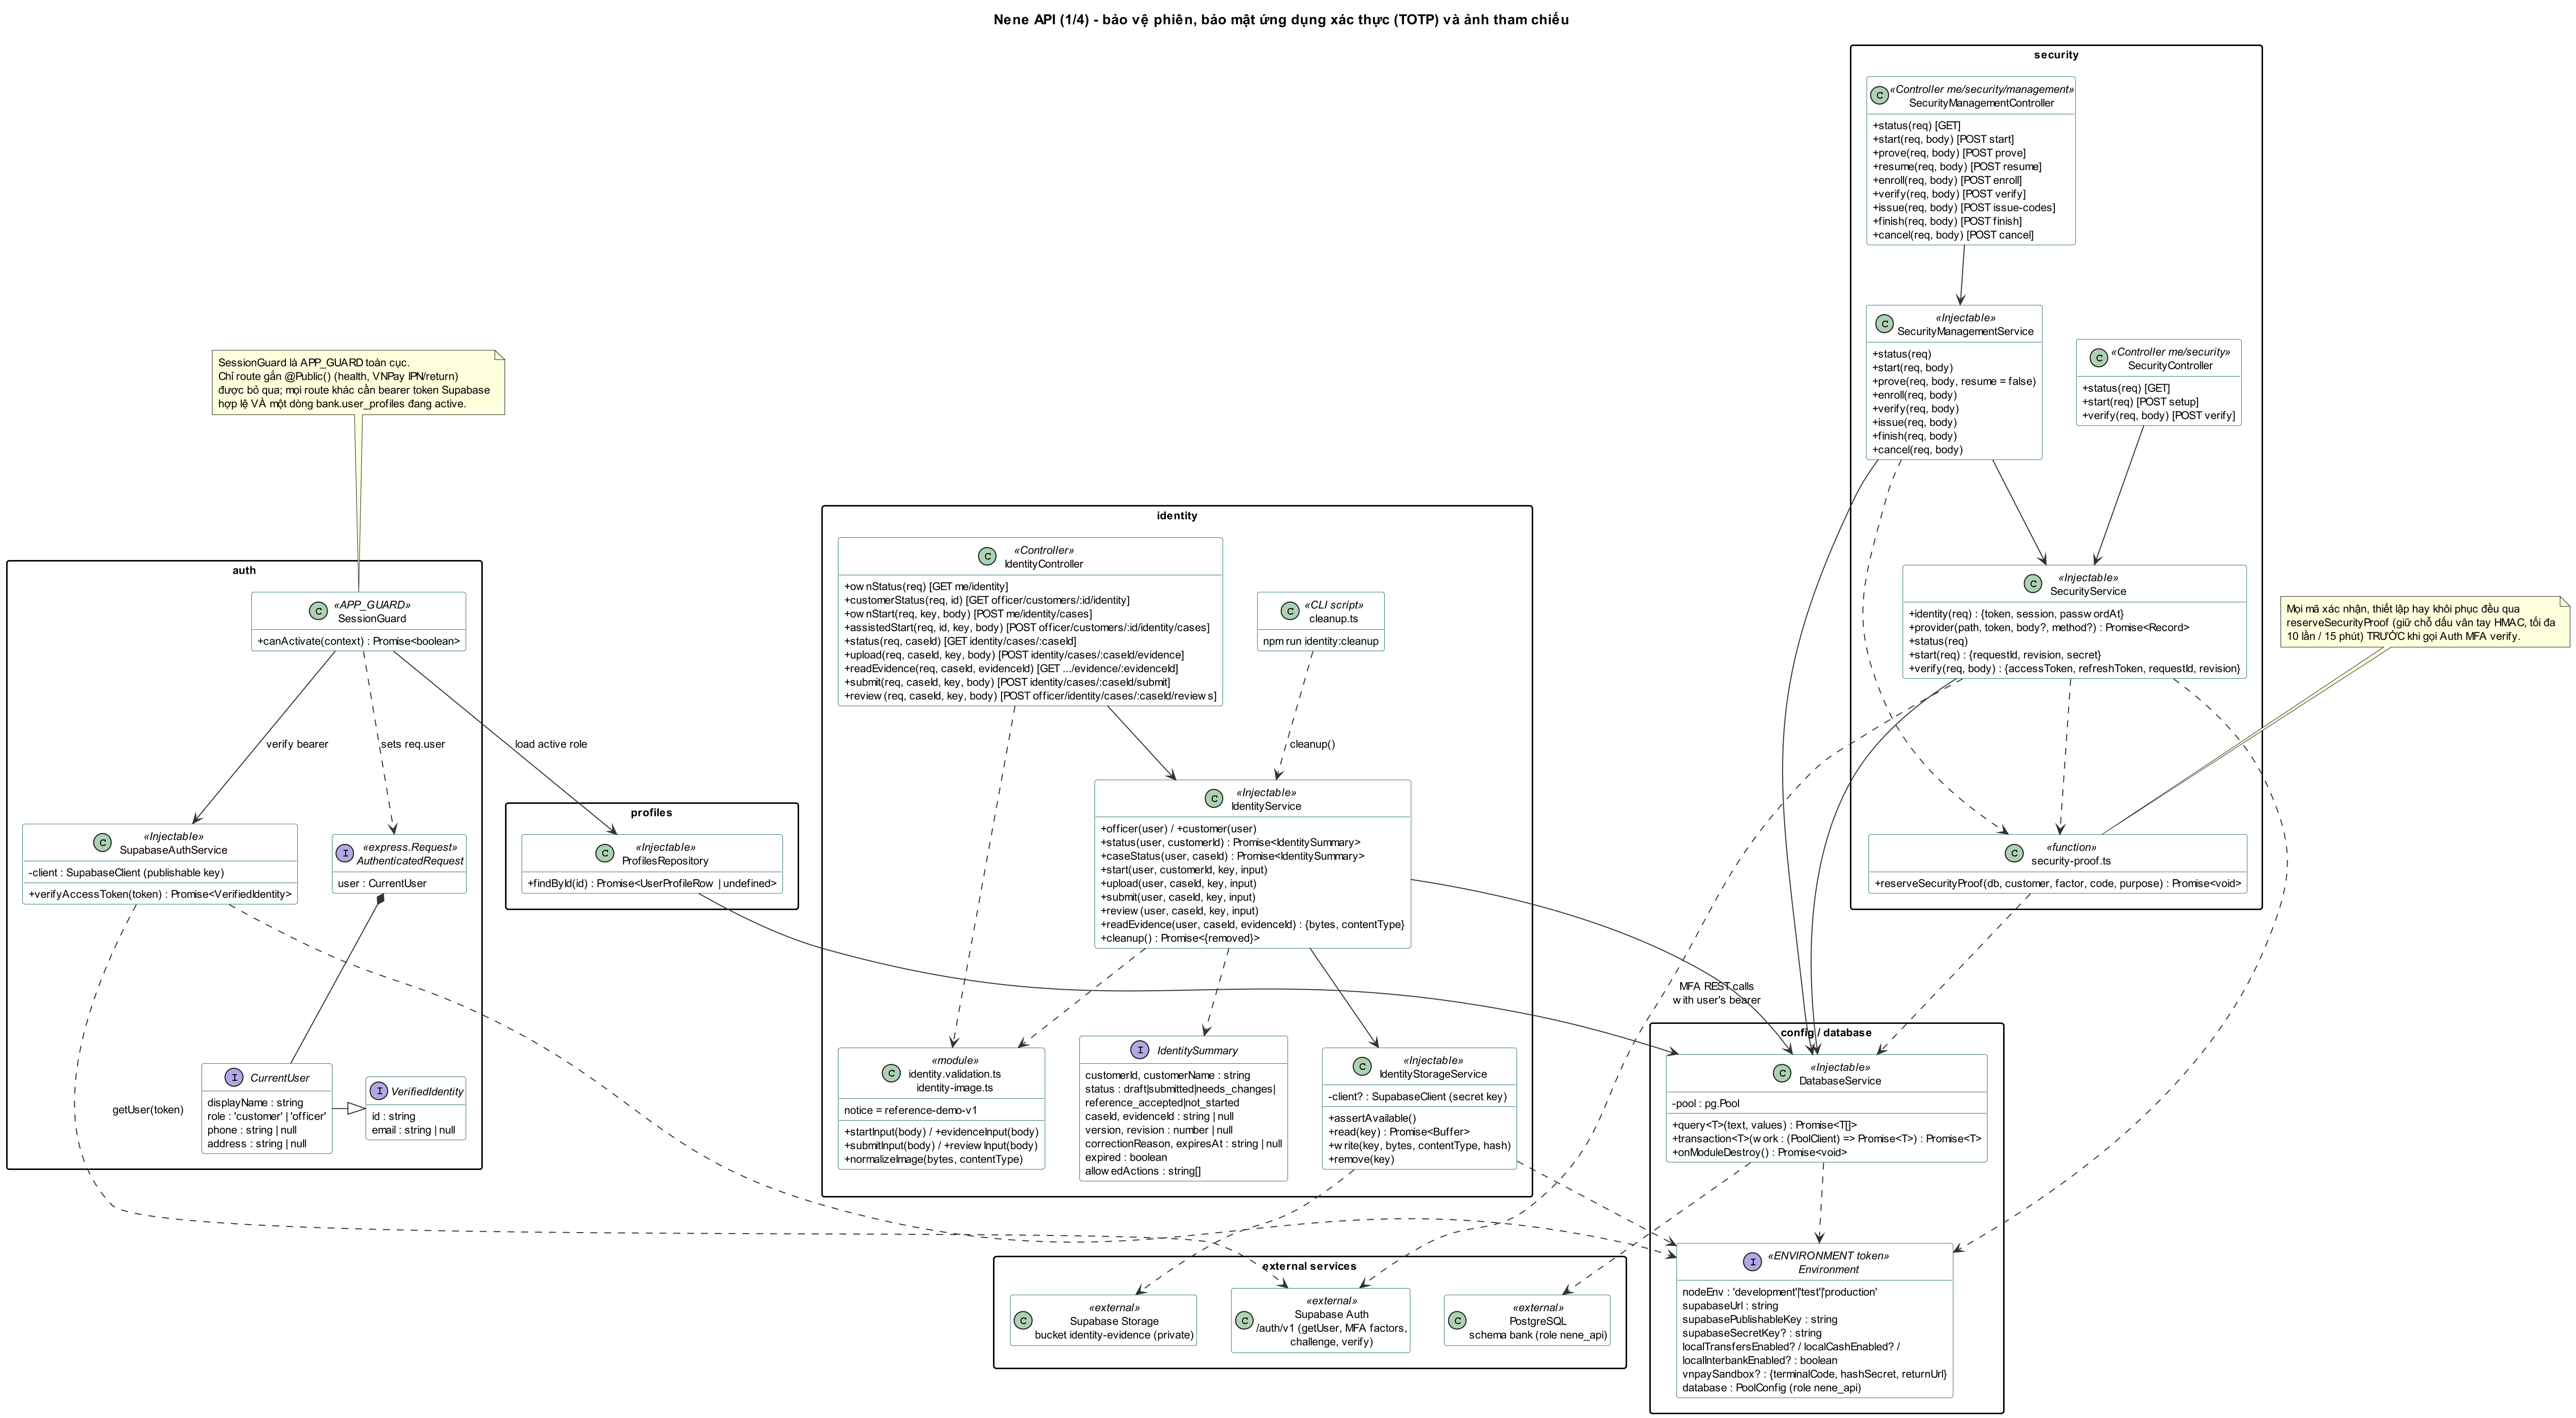
\includegraphics[angle=90,width=\textwidth,height=0.8\textheight,keepaspectratio]{picture/ch2/class-backend-security}
\caption{Biểu đồ lớp backend (1/4): bảo vệ phiên, ứng dụng xác thực và ảnh tham chiếu}
\label{fig:ch2-class-backend-security}
\end{figure}

Hình~\ref{fig:ch2-class-backend-security} là nền tảng mà mọi phần khác dựa vào.
\begin{itemize}
  \item \texttt{SessionGuard} phụ thuộc \texttt{Supabase\allowbreak{}Auth\allowbreak{}Service} (gọi \texttt{getUser} bằng khoá công khai để xác minh token) và \texttt{Profiles\allowbreak{}Repository} (đọc hồ sơ đang hoạt động), rồi gắn \texttt{CurrentUser} vào \texttt{Authenticated\allowbreak{}Request}. \texttt{CurrentUser} mở rộng \texttt{Verified\allowbreak{}Identity} với tên, vai trò và thông tin liên hệ, và là đối tượng mà mọi controller nhận được.
  \item \texttt{Database\allowbreak{}Service} bao bọc \texttt{pg.\allowbreak{}Pool} và là phụ thuộc chung của hầu hết service; giao diện \texttt{Environment} được tiêm qua token \texttt{ENVIRONMENT}.
  \item \texttt{Security\allowbreak{}Controller}/\texttt{Security\allowbreak{}Service} xử lý thiết lập TOTP lần đầu bằng cách gọi API MFA của Supabase thay mặt người dùng; \texttt{Security\allowbreak{}Service} còn cung cấp hai hàm dùng chung cho các phần khác: \texttt{identity(req)} (khách hàng, phiên, thời điểm nhập mật khẩu) và \texttt{provider(...)} (gọi REST Supabase Auth). \texttt{Security\allowbreak{}Management\allowbreak{}Controller}/\texttt{Security\allowbreak{}Management\allowbreak{}Service} cung cấp chín route (trạng thái, bắt đầu, chứng minh, tiếp tục, đăng ký factor mới, xác minh, cấp mã, hoàn tất, huỷ) cho việc thay thế, khôi phục authenticator và cấp mã khôi phục; service này phụ thuộc \texttt{Security\allowbreak{}Service}.
  \item Hàm \texttt{reserve\allowbreak{}Security\allowbreak{}Proof} là điểm chống phát lại mã duy nhất, được cả thiết lập, quản lý authenticator và mọi xác nhận giao dịch gọi.
  \item \texttt{Identity\allowbreak{}Controller} có chín route cho cả khách hàng (\texttt{me/\allowbreak{}identity}) và nhân viên (\texttt{officer/\allowbreak{}...}); \texttt{Identity\allowbreak{}Service} điều phối hồ sơ, lệnh, duyệt và dọn dẹp; \texttt{Identity\allowbreak{}Storage\allowbreak{}Service} là lớp duy nhất chạm vào Supabase Storage bằng khoá bí mật. Các hàm kiểm tra đầu vào và \texttt{normalize\allowbreak{}Image} (giải mã, xoay, mã hoá lại ảnh, bỏ EXIF/GPS, tính SHA-256) được tách thành module thuần. Script \texttt{cleanup.\allowbreak{}ts} chạy thủ công để xoá vật lý ảnh hết hạn.
\end{itemize}

\subsubsection{Khách hàng, hồ sơ và tài khoản}

\begin{figure}[H]
\centering
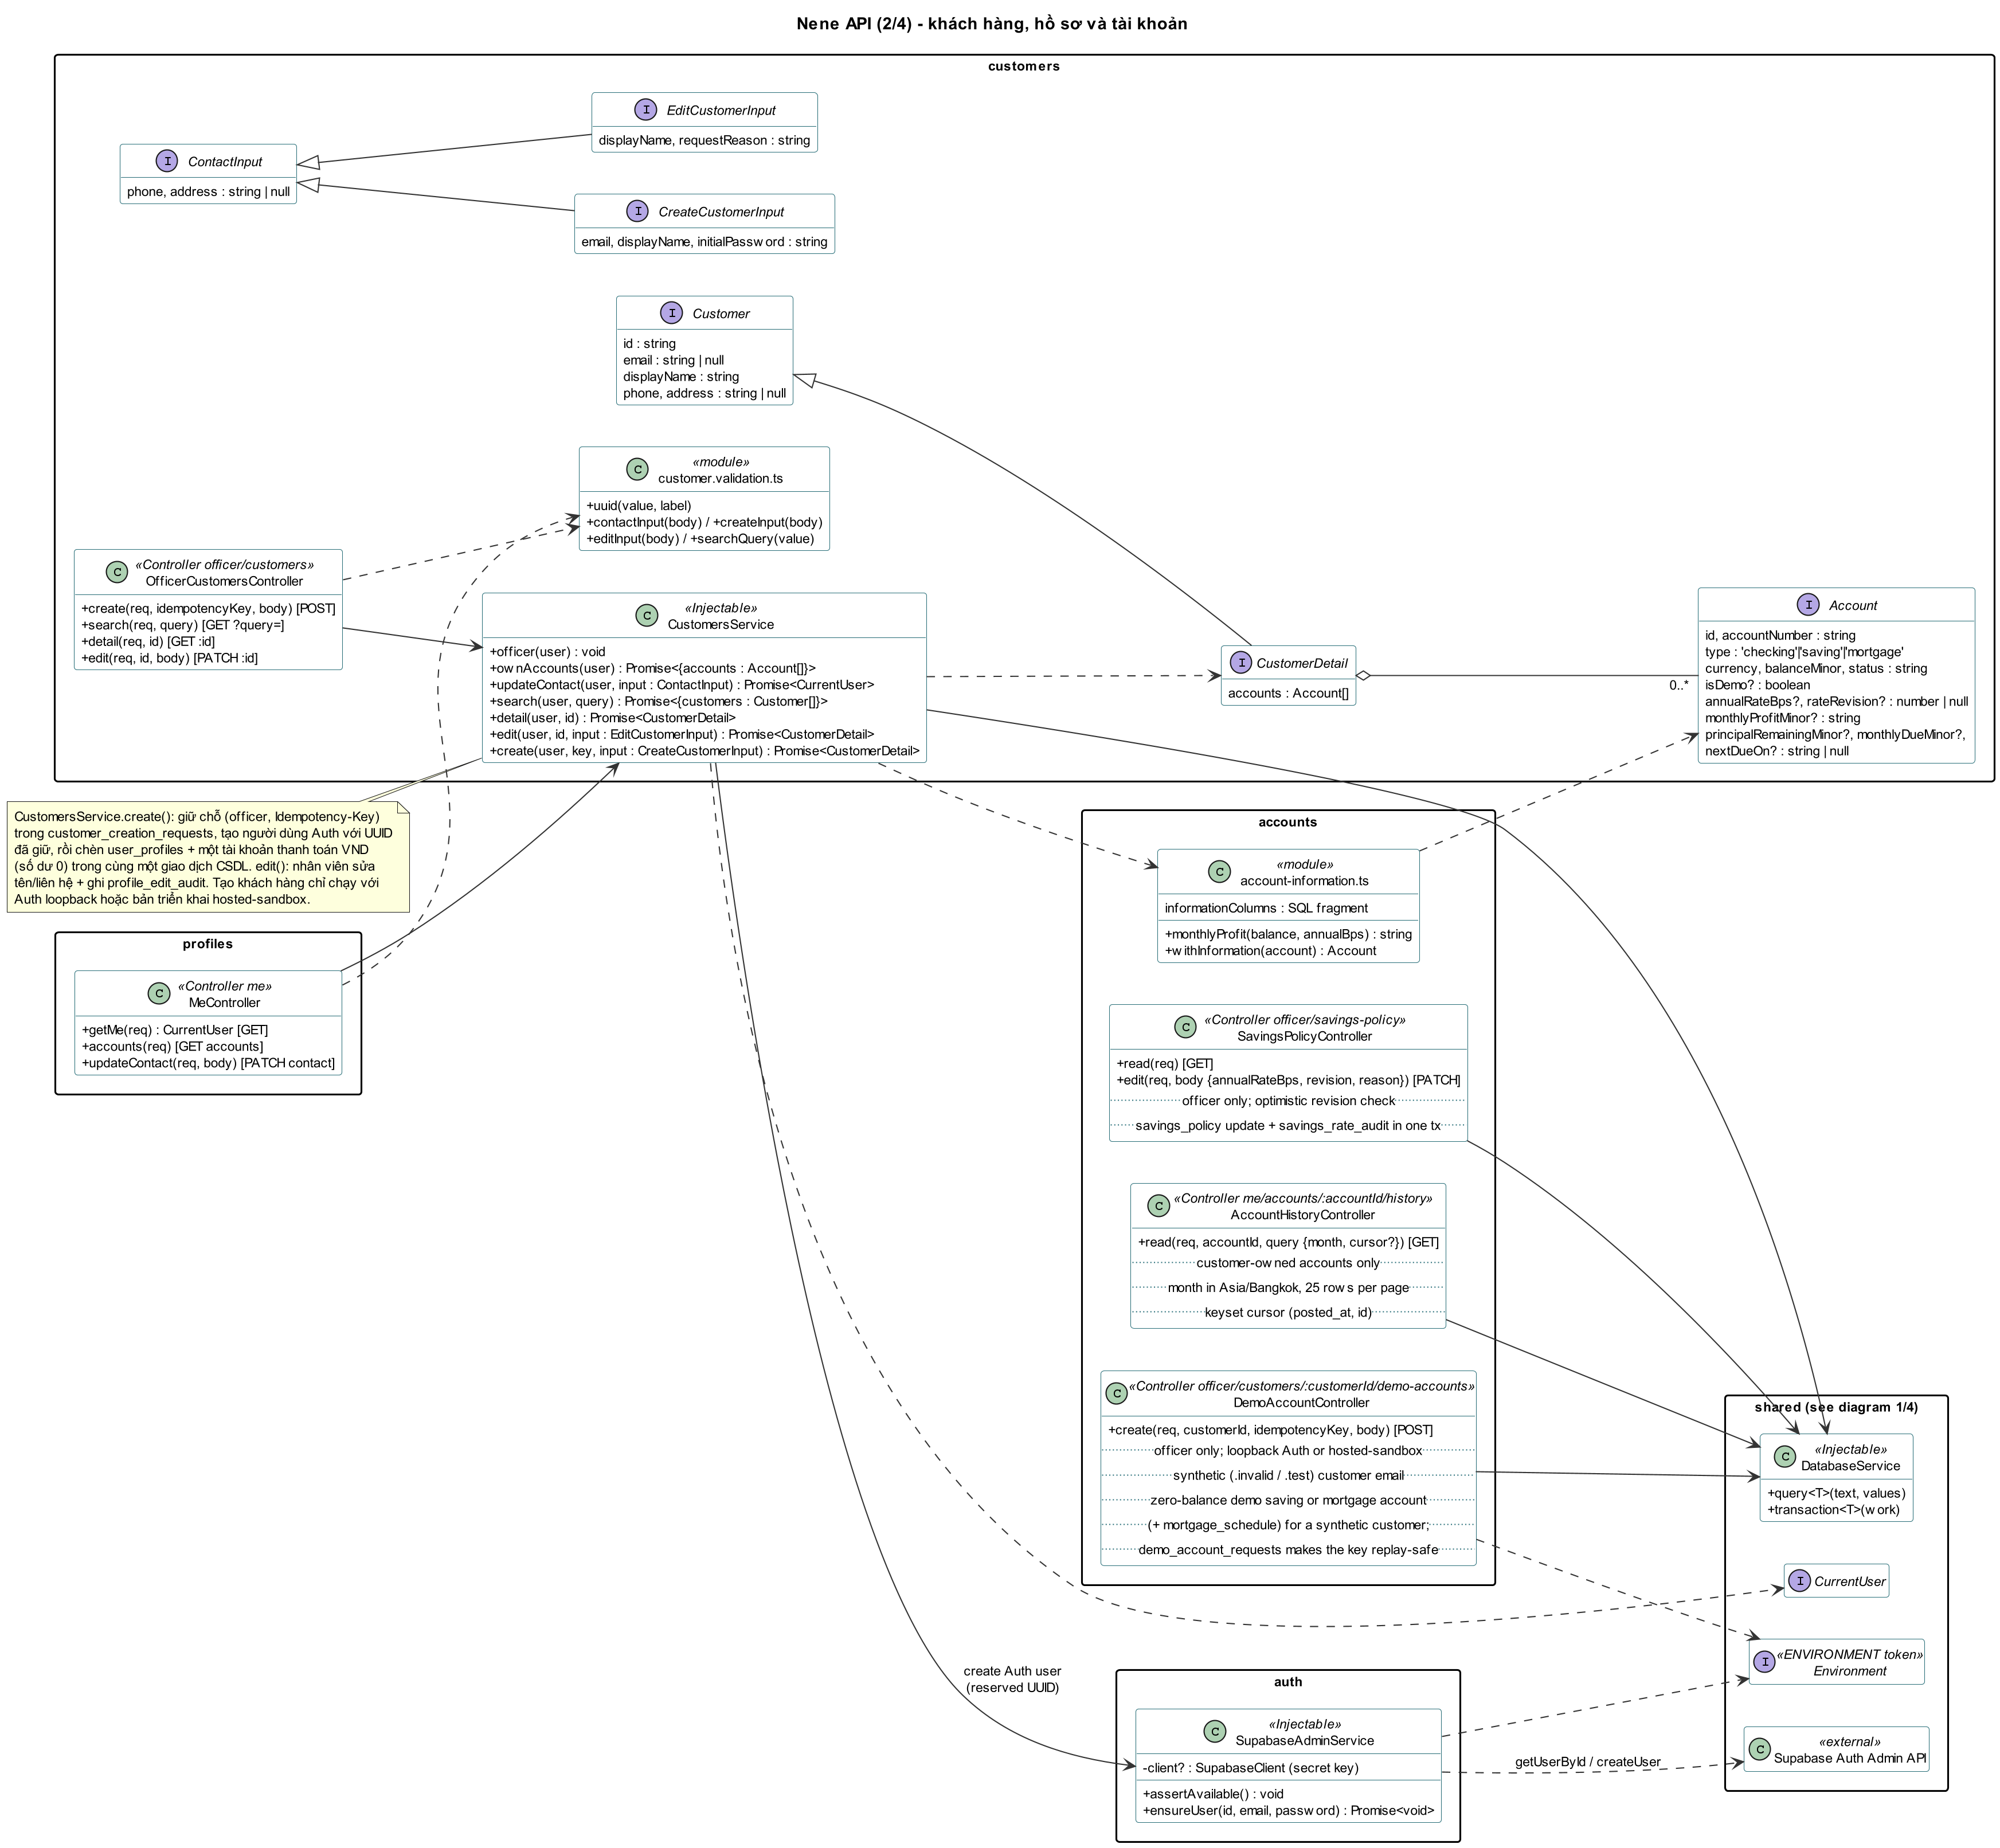
\includegraphics[width=\textwidth,height=0.8\textheight,keepaspectratio]{picture/ch2/class-backend-banking}
\caption{Biểu đồ lớp backend (2/4): khách hàng, hồ sơ và tài khoản}
\label{fig:ch2-class-backend-banking}
\end{figure}

Trong Hình~\ref{fig:ch2-class-backend-banking}, hai controller \texttt{MeController} (khách hàng: \texttt{GET me}, \texttt{GET me/\allowbreak{}accounts}, \texttt{PATCH me/\allowbreak{}contact}) và \texttt{Officer\allowbreak{}Customers\allowbreak{}Controller} (nhân viên: tạo, tìm, xem, sửa) cùng uỷ quyền cho \texttt{Customers\allowbreak{}Service}. Service này phụ thuộc \texttt{Database\allowbreak{}Service} và \texttt{Supabase\allowbreak{}Admin\allowbreak{}Service} --- lớp duy nhất tạo người dùng Supabase Auth với UUID đã giữ chỗ (\texttt{ensureUser}). Các giao diện dữ liệu trao đổi (DTO) thể hiện quan hệ: \texttt{Customer\allowbreak{}Detail} kế thừa \texttt{Customer} và kết tập 0..* \texttt{Account}; \texttt{Create\allowbreak{}Customer\allowbreak{}Input} và \texttt{Edit\allowbreak{}Customer\allowbreak{}Input} kế thừa \texttt{ContactInput}. \texttt{Account} có các trường tuỳ chọn theo loại: lãi suất và lợi nhuận tháng cho tài khoản tiết kiệm, dư nợ, khoản trả hằng tháng, ngày đến hạn cho tài khoản vay. Các trường số tiền được truyền dưới dạng chuỗi để tránh mất độ chính xác của số trong JavaScript. Module \texttt{account-\allowbreak{}information.\allowbreak{}ts} chứa công thức lợi nhuận tháng (\texttt{monthlyProfit}) và đoạn SQL dùng chung để nạp thông tin theo loại tài khoản. Ba controller \texttt{Account\allowbreak{}History\allowbreak{}Controller}, \texttt{Savings\allowbreak{}Policy\allowbreak{}Controller}, \texttt{Demo\allowbreak{}Account\allowbreak{}Controller} làm việc trực tiếp với \texttt{Database\allowbreak{}Service} như đã giải thích ở Mục~\ref{sec:ch2-layers}.

\subsubsection{Xác nhận giao dịch, chuyển khoản, tiền mặt và liên ngân hàng}

\begin{figure}[H]
\centering
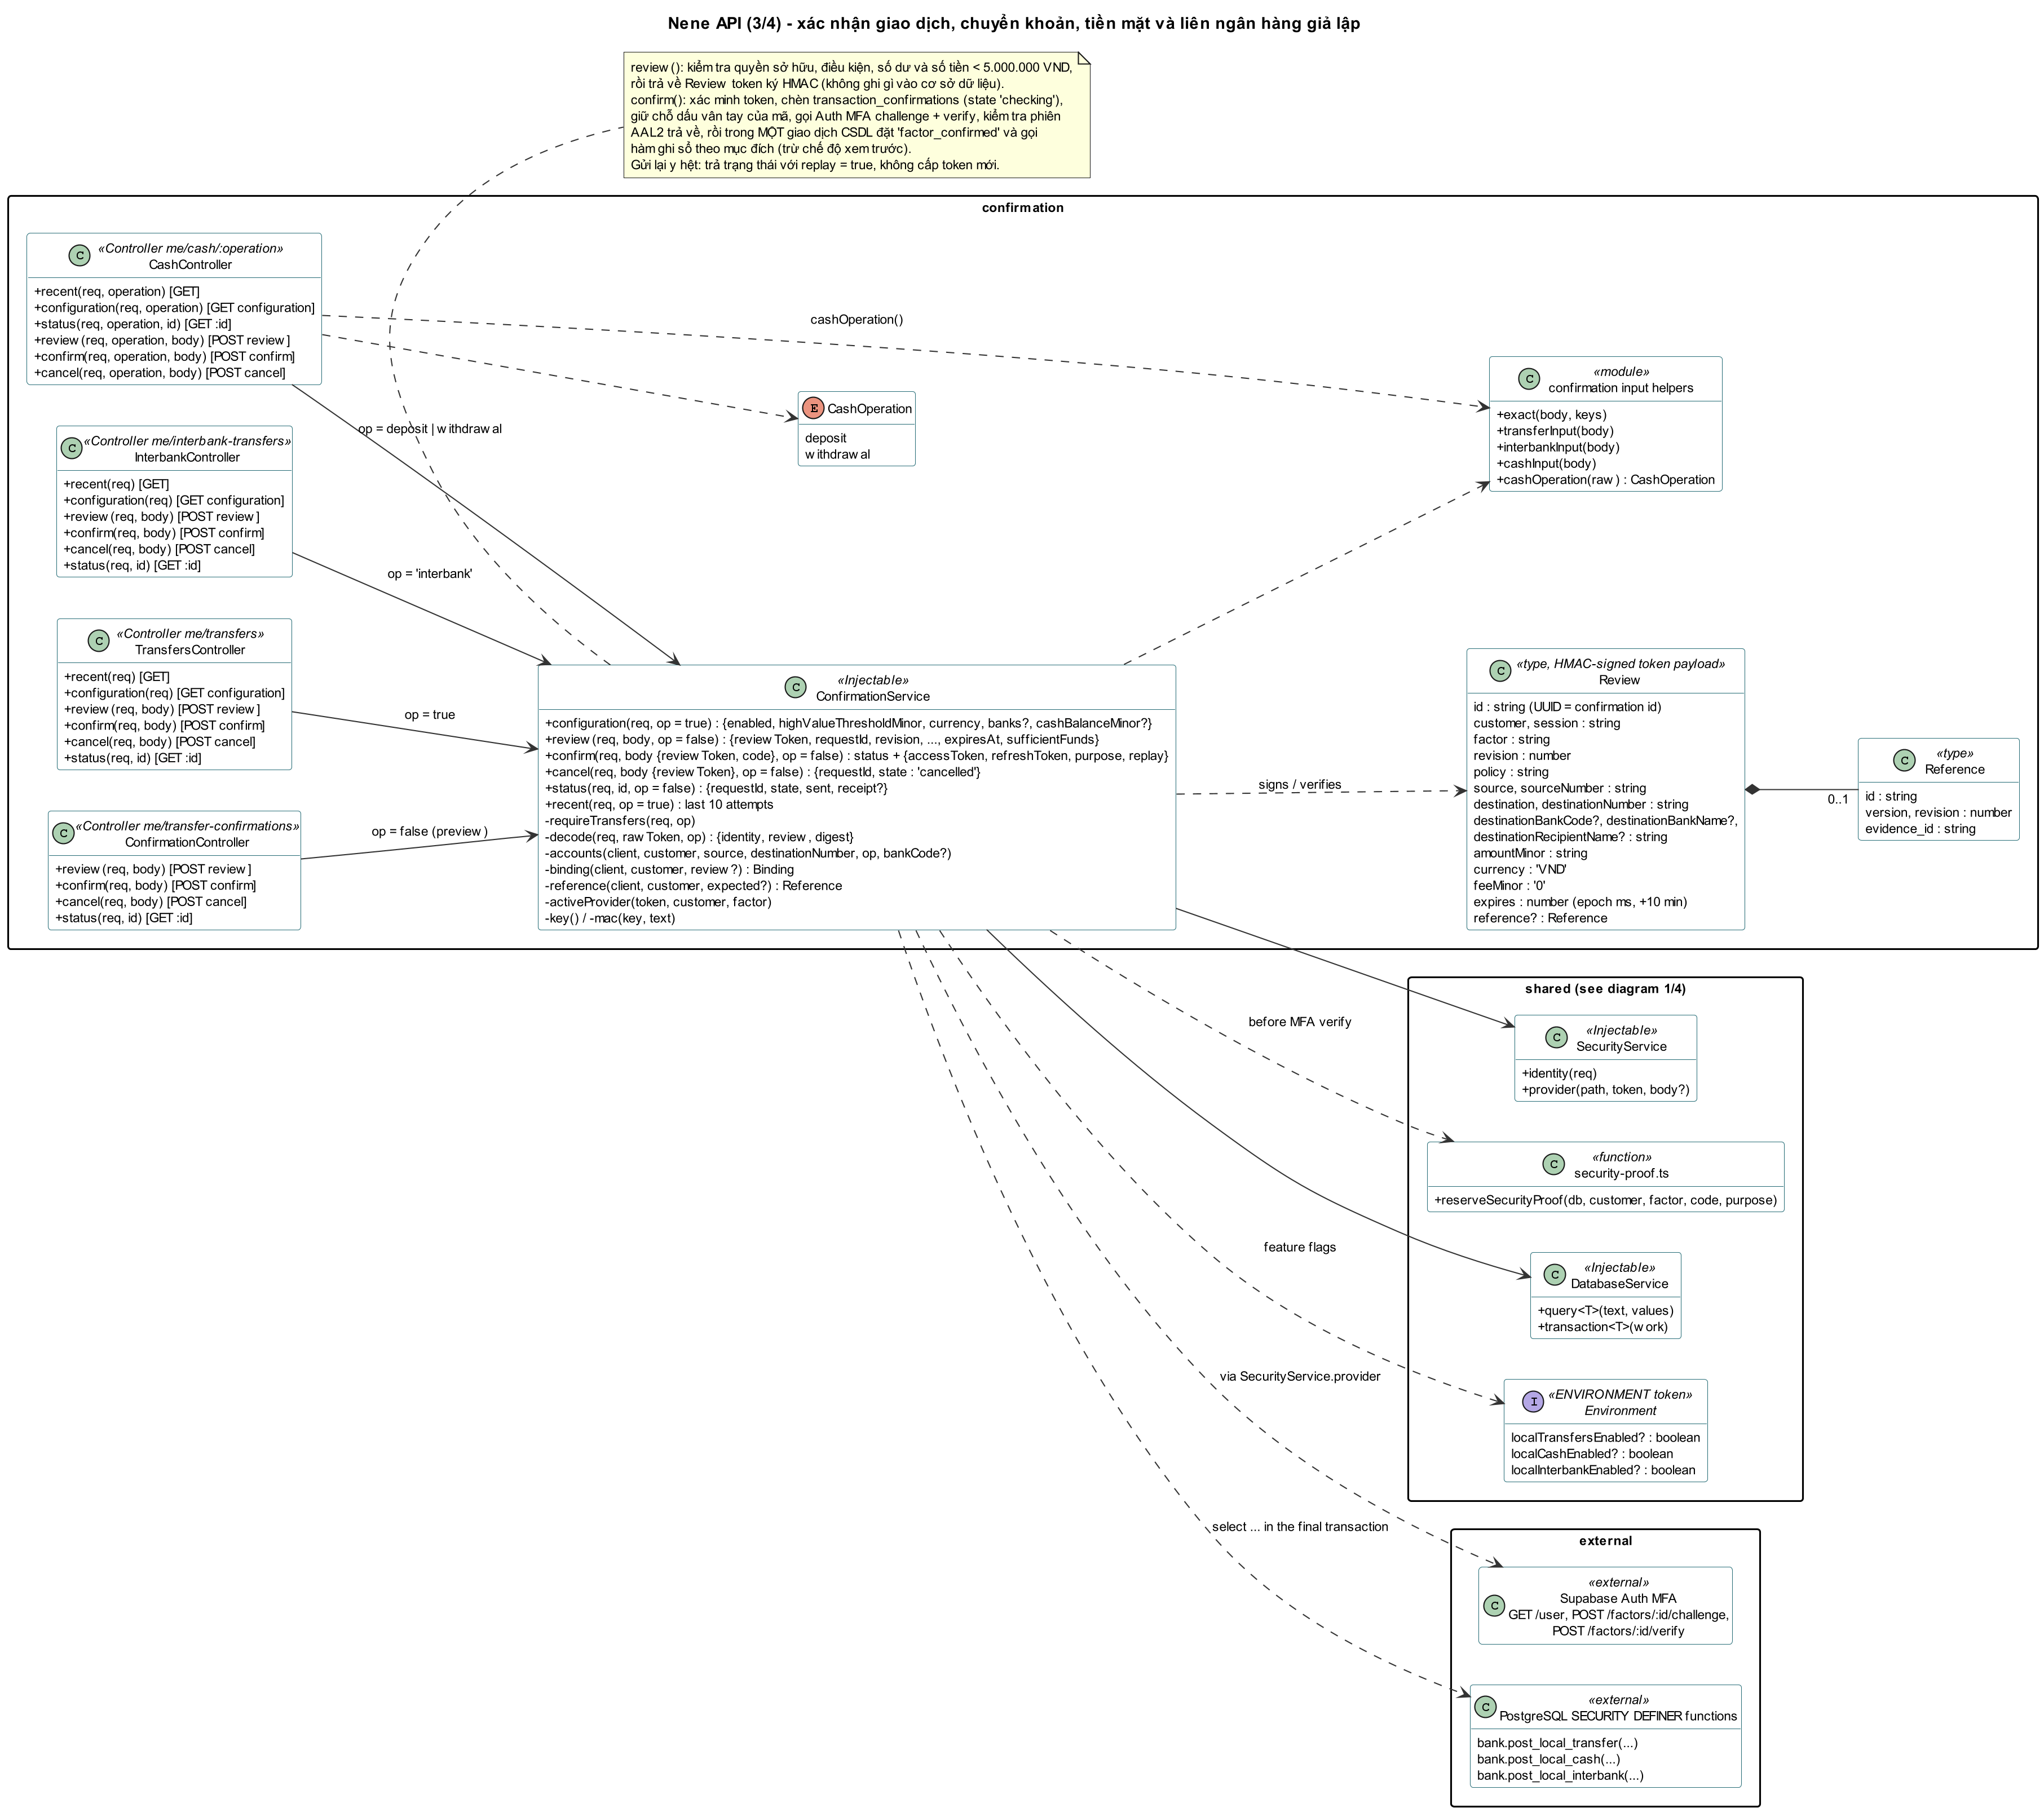
\includegraphics[width=\textwidth,height=0.8\textheight,keepaspectratio]{picture/ch2/class-backend-transactions}
\caption{Biểu đồ lớp backend (3/4): bộ máy xác nhận giao dịch dùng chung}
\label{fig:ch2-class-backend-transactions}
\end{figure}

Hình~\ref{fig:ch2-class-backend-transactions} thể hiện quyết định thiết kế quan trọng nhất về giao dịch: \emph{một} \texttt{Confirmation\allowbreak{}Service} phục vụ bốn controller. Mỗi controller truyền một tham số \texttt{Operation} khác nhau: \texttt{false} cho xem trước (\texttt{Confirmation\allowbreak{}Controller}), \texttt{true} cho chuyển khoản trong Nene (\texttt{Transfers\allowbreak{}Controller}), \texttt{'deposit'}/\texttt{'withdrawal'} cho tiền mặt (\texttt{Cash\allowbreak{}Controller}) và \texttt{'interbank'} cho liên ngân hàng mô phỏng (\texttt{Interbank\allowbreak{}Controller}). Từ tham số này service suy ra mục đích ghi trong \texttt{transaction\_\allowbreak{}confirmations}, policy của review, mục đích trao đổi phiên và hàm ghi sổ cần gọi. Cách tổ chức này giống mẫu Strategy được tham số hoá: phần bảo mật (giải mã và kiểm tra \texttt{Review}, giữ chỗ mã, gọi Supabase MFA, kiểm tra AAL2, quản lý trạng thái) chỉ viết một lần, nên không có luồng tiền nào có thể vô tình thiếu bước 2FA. Lớp \texttt{Review} là nội dung của token đã ký và hợp thành 0..1 \texttt{Reference} (hồ sơ ảnh tham chiếu đã chấp nhận, kèm version, revision, evidence). \texttt{Confirmation\allowbreak{}Service} phụ thuộc \texttt{Security\allowbreak{}Service}, \texttt{reserve\allowbreak{}Security\allowbreak{}Proof}, \texttt{Database\allowbreak{}Service} và các cờ bật/tắt trong \texttt{Environment}, và gọi ba hàm ghi sổ \texttt{SECURITY DEFINER} trong PostgreSQL.

\subsubsection{Thanh toán sandbox, chi nhánh, trợ lý và health}

\begin{figure}[H]
\centering
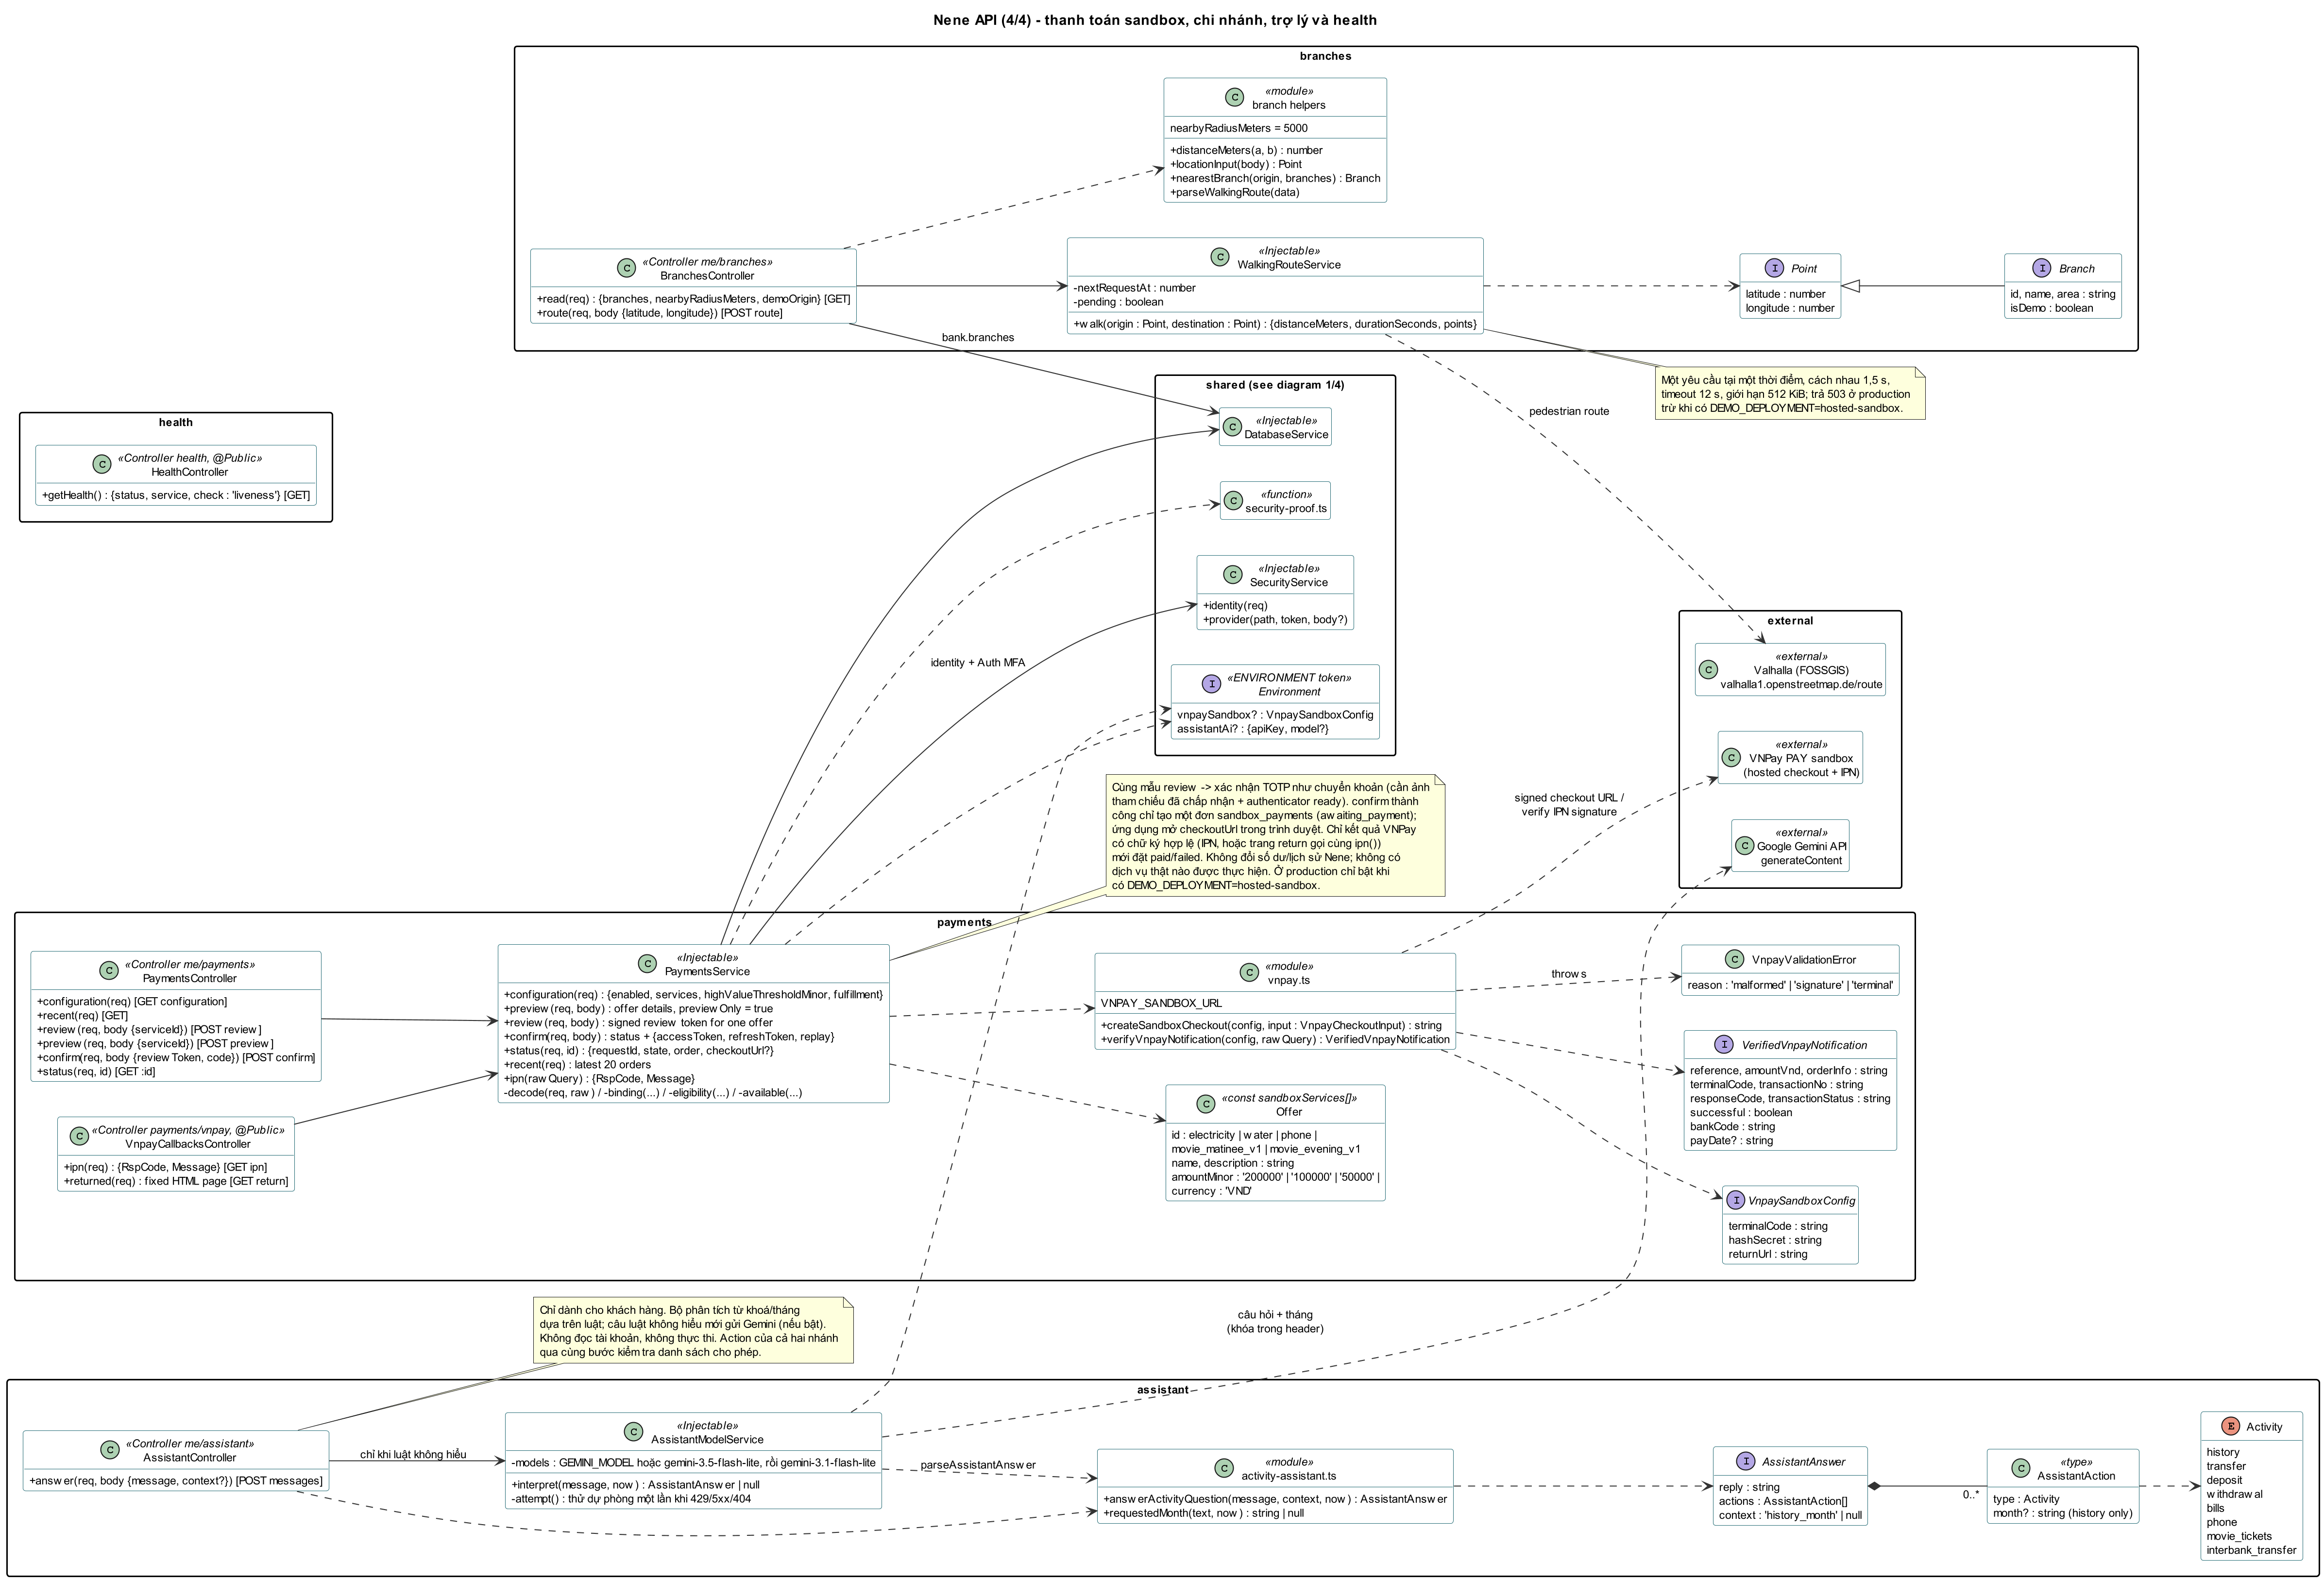
\includegraphics[width=\textwidth,height=0.8\textheight,keepaspectratio]{picture/ch2/class-backend-services}
\caption{Biểu đồ lớp backend (4/4): thanh toán VNPay sandbox, chi nhánh, trợ lý và health}
\label{fig:ch2-class-backend-services}
\end{figure}

Hình~\ref{fig:ch2-class-backend-services} gồm ba nhóm độc lập.
\begin{itemize}
  \item \textbf{Thanh toán}: \texttt{Payments\allowbreak{}Controller} (sáu route cho khách hàng) và \texttt{Vnpay\allowbreak{}Callbacks\allowbreak{}Controller} (\texttt{@Public}, hai route \texttt{ipn} và \texttt{return}) cùng dùng \texttt{Payments\allowbreak{}Service}. Service này lặp lại mẫu review $\rightarrow$ xác nhận TOTP của giao dịch tiền (dùng \texttt{Security\allowbreak{}Service} và \texttt{reserve\allowbreak{}Security\allowbreak{}Proof}) nhưng kết quả là một đơn chờ thanh toán chứ không thay đổi số dư. Module \texttt{vnpay.\allowbreak{}ts} gồm các hàm thuần \texttt{create\allowbreak{}Sandbox\allowbreak{}Checkout} và \texttt{verify\allowbreak{}Vnpay\allowbreak{}Notification}, tách biệt hoàn toàn khỏi HTTP và cơ sở dữ liệu nên dễ kiểm thử; lỗi xác minh được biểu diễn bằng \texttt{Vnpay\allowbreak{}Validation\allowbreak{}Error} với lý do \texttt{malformed}, \texttt{signature} hoặc \texttt{terminal}. Danh mục dịch vụ \texttt{Offer} là hằng số phía máy chủ, khách hàng không thể tự đặt giá.
  \item \textbf{Chi nhánh}: \texttt{Branches\allowbreak{}Controller} đọc bảng \texttt{bank.\allowbreak{}branches}, dùng các hàm thuần \texttt{distance\allowbreak{}Meters} (công thức haversine), \texttt{nearestBranch} (bán kính 5~km) và \texttt{Walking\allowbreak{}Route\allowbreak{}Service} để gọi Valhalla. Service này giới hạn một yêu cầu tại một thời điểm, cách nhau 1,5 giây, timeout 12 giây, phản hồi tối đa 512~KiB, để tôn trọng giới hạn của máy chủ công cộng.
  \item \textbf{Trợ lý}: \texttt{Assistant\allowbreak{}Controller} chỉ cho khách hàng, gọi hàm \texttt{answer\allowbreak{}Activity\allowbreak{}Question} trong \texttt{activity-\allowbreak{}assistant.\allowbreak{}ts}. Kết quả \texttt{Assistant\allowbreak{}Answer} gồm câu trả lời và 0..* \texttt{Assistant\allowbreak{}Action}, mỗi action thuộc một trong tám giá trị của enum \texttt{Activity}. Trợ lý không đọc tài khoản và không thực thi giao dịch. Khi luật không hiểu câu hỏi và tính năng được bật, \texttt{Assistant\allowbreak{}Model\allowbreak{}Service} (Hình~\ref{fig:ch2-class-backend-services}) gửi riêng câu hỏi và tháng hiện tại tới Gemini API; kết quả phải qua cùng hàm kiểm tra \texttt{parse\allowbreak{}Assistant\allowbreak{}Answer}, nên mô hình cũng chỉ có thể đề xuất các action thuộc enum \texttt{Activity}.
  \item \texttt{Health\allowbreak{}Controller} là route công khai cho kiểm tra sức khoẻ của Render.
\end{itemize}

\subsection{Ứng dụng Flutter}
\label{sec:ch2-class-app}

\subsubsection{Khung ứng dụng, phiên đăng nhập và luồng khách hàng/nhân viên}

\begin{figure}[H]
\centering
\includegraphics[width=\textwidth,height=0.8\textheight,keepaspectratio]{picture/ch2/class-app-core}
\caption{Biểu đồ lớp ứng dụng (1/3): khung ứng dụng, phiên và luồng tài khoản}
\label{fig:ch2-class-app-core}
\end{figure}

Hình~\ref{fig:ch2-class-app-core} chia làm ba gói theo tầng. \texttt{NeneApp} lắng nghe \texttt{Session\allowbreak{}Controller} và hiển thị \texttt{SignInScreen} khi chưa đăng nhập hoặc \texttt{Customer\allowbreak{}Workspace} khi phiên sẵn sàng. \texttt{Customer\allowbreak{}Workspace} là một widget duy nhất cho cả hai vai trò; nó chọn trang trong enum \texttt{\_\allowbreak{}Page} (17 trang) theo vai trò server trả về, và hợp thành một \texttt{Customer\allowbreak{}Flow\allowbreak{}Controller} riêng. Khi đăng xuất hoặc phiên hết hạn, cả không gian làm việc bị huỷ nên không còn trang được bảo vệ nào sót lại.

\texttt{Session\allowbreak{}Controller} phụ thuộc hai giao diện \texttt{Auth\allowbreak{}Repository} và \texttt{Profile\allowbreak{}Repository}. \texttt{Owned\allowbreak{}Auth\allowbreak{}Repository} cài đặt \texttt{Auth\allowbreak{}Repository} bằng cách uỷ quyền cho \texttt{SessionOwner}; \texttt{SessionOwner} lại phụ thuộc giao diện \texttt{AuthPort} (cài đặt bởi \texttt{Supabase\allowbreak{}Auth\allowbreak{}Port} gọi REST Supabase Auth) và kết tập một \texttt{OwnedSession} chỉ trong bộ nhớ. \texttt{Customer\allowbreak{}Flow\allowbreak{}Controller} dùng \texttt{Session\allowbreak{}Controller.\allowbreak{}authorized()} để lấy token và gọi \texttt{Banking\allowbreak{}Repository} (cài đặt bởi \texttt{BankingApi}). Các lớp dữ liệu \texttt{UserProfile}, \texttt{BankAccount}, \texttt{Customer\allowbreak{}Detail} (kết tập nhiều \texttt{BankAccount}) và \texttt{CustomerDraft} là bản sao phía client của DTO ở backend.

\subsubsection{Bảo mật giao dịch, xác nhận và thanh toán sandbox}

\begin{figure}[H]
\centering
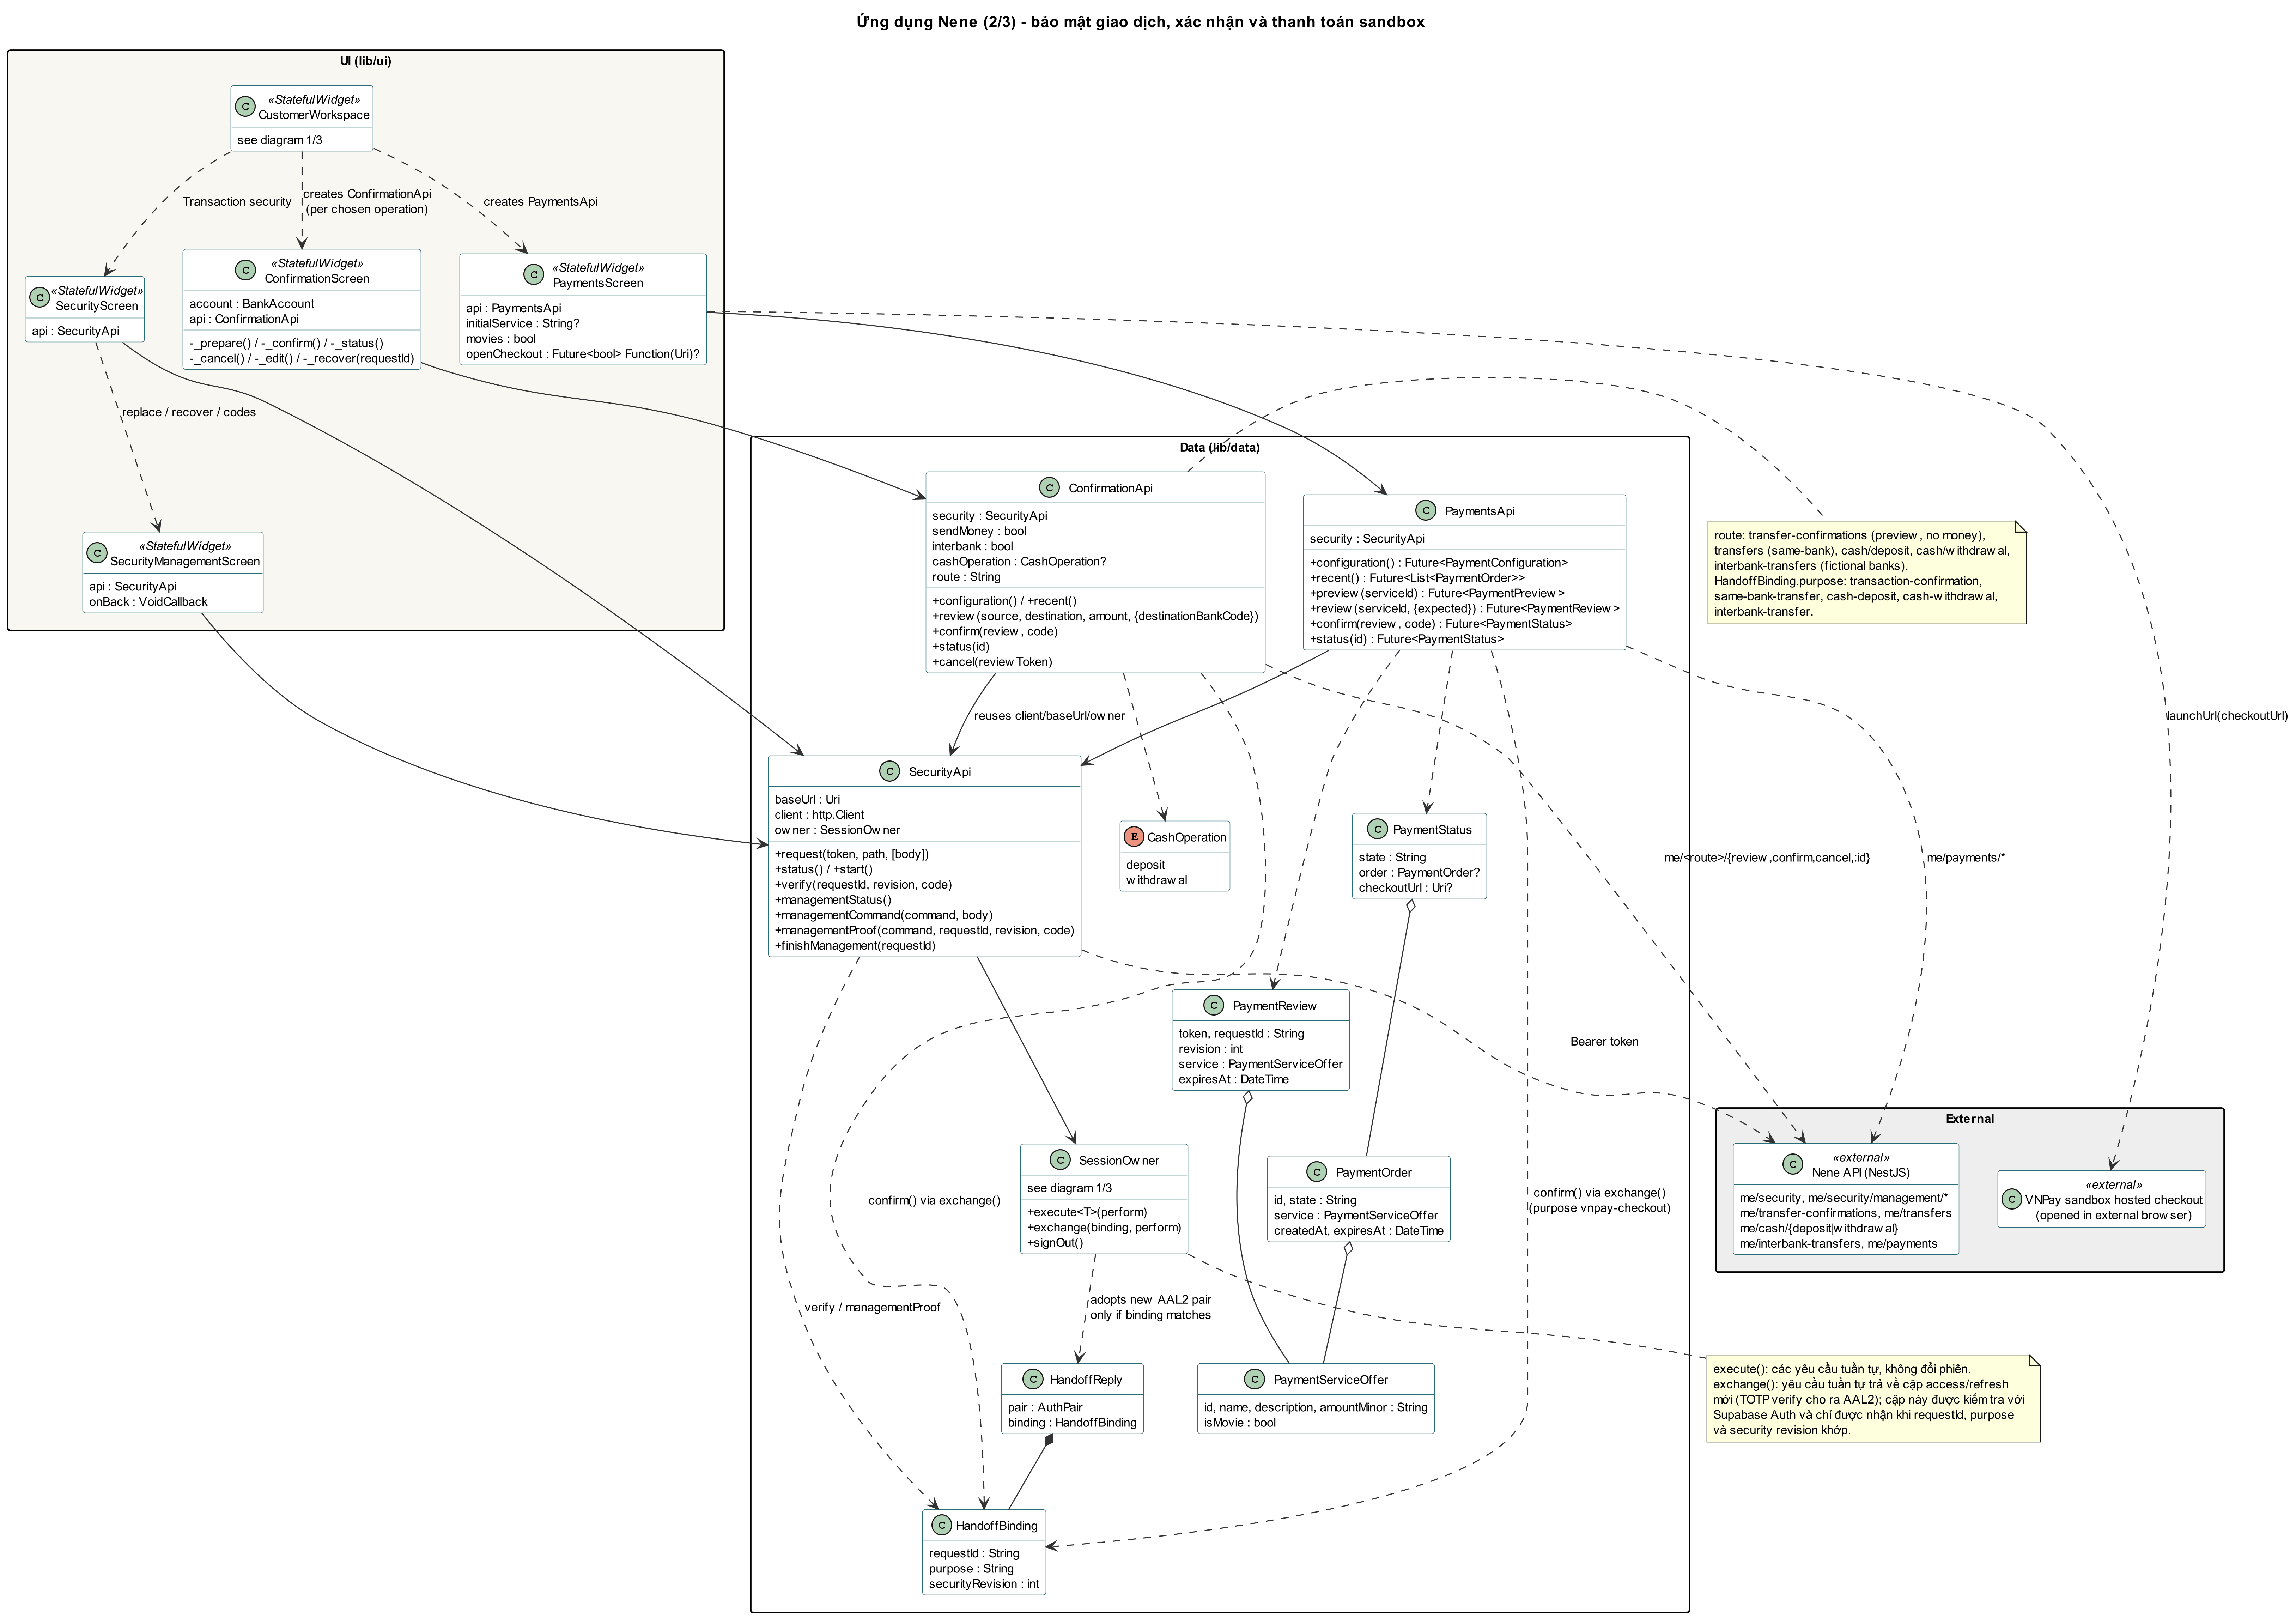
\includegraphics[angle=90,width=\textwidth,height=0.8\textheight,keepaspectratio]{picture/ch2/class-app-transactions}
\caption{Biểu đồ lớp ứng dụng (2/3): bảo mật giao dịch, xác nhận và thanh toán sandbox}
\label{fig:ch2-class-app-transactions}
\end{figure}

Trong Hình~\ref{fig:ch2-class-app-transactions}, \texttt{SecurityApi} là client nền tảng của mọi thao tác cần TOTP: nó giữ \texttt{baseUrl}, \texttt{http.\allowbreak{}Client} và tham chiếu tới \texttt{SessionOwner}. \texttt{Confirmation\allowbreak{}Api} và \texttt{PaymentsApi} tái sử dụng \texttt{SecurityApi}. Tương ứng với \texttt{Confirmation\allowbreak{}Service} dùng chung ở backend, \texttt{Confirmation\allowbreak{}Screen} và \texttt{Confirmation\allowbreak{}Api} là một cặp dùng chung cho xem trước, chuyển khoản, nạp, rút và liên ngân hàng; \texttt{Customer\allowbreak{}Workspace} chỉ tạo \texttt{Confirmation\allowbreak{}Api} với route và mục đích phù hợp (ví dụ \texttt{transfers} với \texttt{same-\allowbreak{}bank-\allowbreak{}transfer}). Khi xác nhận, các API gọi \texttt{SessionOwner.\allowbreak{}exchange()} kèm một \texttt{Handoff\allowbreak{}Binding} (\texttt{requestId}, \texttt{purpose}, \texttt{security\allowbreak{}Revision}); \texttt{HandoffReply} hợp thành binding trả về và chỉ được nhận khi khớp. \texttt{Payments\allowbreak{}Screen} mở \texttt{checkoutUrl} của VNPay trong trình duyệt ngoài sau khi kiểm tra đúng máy chủ và đường dẫn HTTPS của sandbox; các lớp \texttt{PaymentReview}, \texttt{PaymentStatus}, \texttt{PaymentOrder} kết tập \texttt{Payment\allowbreak{}Service\allowbreak{}Offer}.

\subsubsection{Ảnh tham chiếu, lịch sử, chi nhánh, trợ lý và công cụ nhân viên}

\begin{figure}[H]
\centering
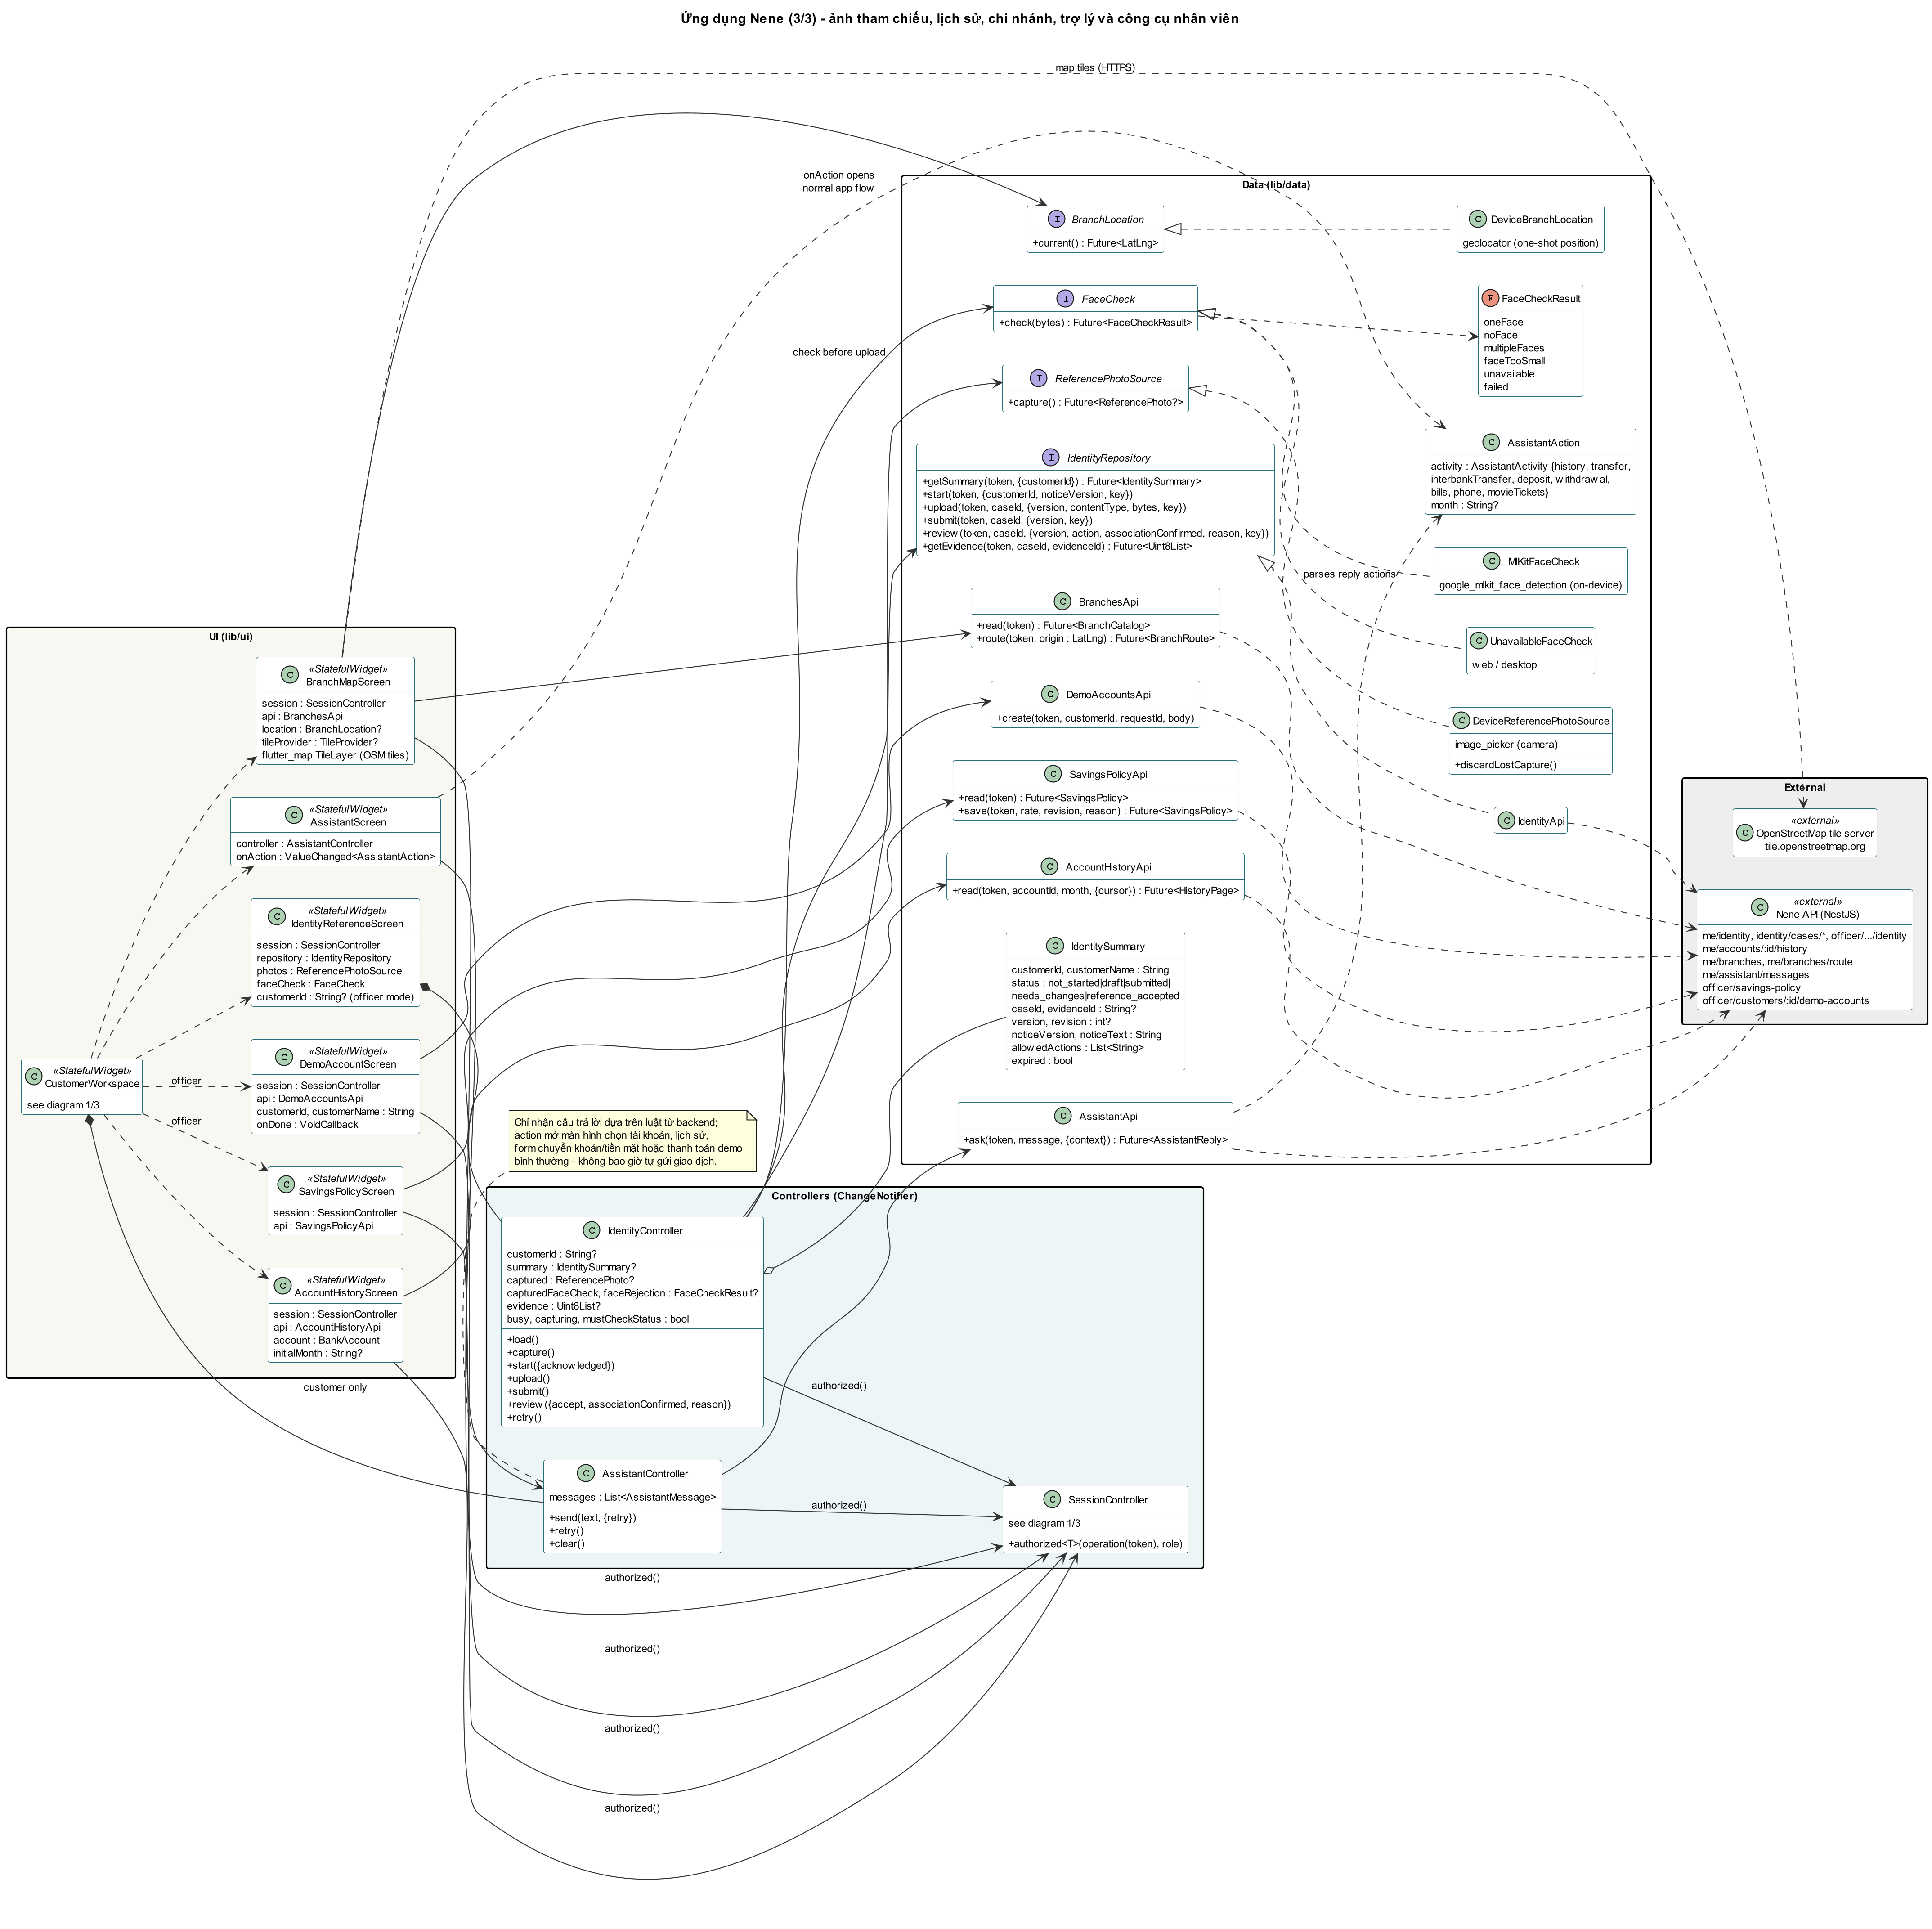
\includegraphics[width=\textwidth,height=0.8\textheight,keepaspectratio]{picture/ch2/class-app-features}
\caption{Biểu đồ lớp ứng dụng (3/3): ảnh tham chiếu, lịch sử, chi nhánh, trợ lý và công cụ nhân viên}
\label{fig:ch2-class-app-features}
\end{figure}

Hình~\ref{fig:ch2-class-app-features} cho thấy cùng một khuôn mẫu lặp lại ở mọi tính năng: màn hình $\rightarrow$ (controller nếu có trạng thái phức tạp) $\rightarrow$ \texttt{Session\allowbreak{}Controller.\allowbreak{}authorized()} $\rightarrow$ API client. \texttt{Identity\allowbreak{}Reference\allowbreak{}Screen} hợp thành \texttt{Identity\allowbreak{}Controller}, controller này phụ thuộc ba giao diện: \texttt{Identity\allowbreak{}Repository} (cài đặt bởi \texttt{IdentityApi}), \texttt{Reference\allowbreak{}Photo\allowbreak{}Source} (cài đặt bởi \texttt{Device\allowbreak{}Reference\allowbreak{}Photo\allowbreak{}Source} dùng \texttt{image\_\allowbreak{}picker}) và \texttt{FaceCheck}. \texttt{FaceCheck} có hai cài đặt: \texttt{Ml\allowbreak{}Kit\allowbreak{}Face\allowbreak{}Check} trên Android/iOS và \texttt{Unavailable\allowbreak{}Face\allowbreak{}Check} trên web và desktop; kết quả là enum \texttt{Face\allowbreak{}Check\allowbreak{}Result} (\texttt{oneFace}, \texttt{noFace}, \texttt{multipleFaces}, \texttt{faceTooSmall}, \texttt{unavailable}, \texttt{failed}). Cùng cách đó, \texttt{Branch\allowbreak{}Map\allowbreak{}Screen} phụ thuộc giao diện \texttt{Branch\allowbreak{}Location} (cài đặt bởi \texttt{Device\allowbreak{}Branch\allowbreak{}Location} dùng \texttt{geolocator}) nên có thể kiểm thử trường hợp bị từ chối quyền vị trí. \texttt{Assistant\allowbreak{}Screen} dùng \texttt{Assistant\allowbreak{}Controller}; mỗi \texttt{Assistant\allowbreak{}Action} chỉ mở luồng bình thường của ứng dụng, không tự gửi giao dịch. Hai màn hình dành cho nhân viên là \texttt{Savings\allowbreak{}Policy\allowbreak{}Screen} và \texttt{Demo\allowbreak{}Account\allowbreak{}Screen}.

% ======================================================================
\section{Thiết kế cơ sở dữ liệu}
\label{sec:ch2-database}

\subsection{Tổ chức schema và tiến trình migration}
\label{sec:ch2-migrations}

Toàn bộ dữ liệu nghiệp vụ nằm trong schema riêng \texttt{bank} của PostgreSQL, tách khỏi các schema do Supabase quản lý (\texttt{auth} cho người dùng và phiên, \texttt{storage} cho tệp). Mật khẩu không bao giờ được lưu trong schema \texttt{bank}: bảng \texttt{bank.\allowbreak{}user\_\allowbreak{}profiles} chỉ tham chiếu \texttt{auth.\allowbreak{}users(id)}. Schema được xây dựng bởi 17 tệp migration SQL áp dụng theo thứ tự tên tệp (Bảng~\ref{tab:ch2-migrations}); mỗi migration tự khai báo tường minh quyền và chính sách cho các đối tượng nó tạo ra.

{\small
\begin{longtable}{>{\raggedright\arraybackslash}p{0.06\textwidth}>{\raggedright\arraybackslash}p{0.36\textwidth}>{\raggedright\arraybackslash}p{0.48\textwidth}}
\caption{Các migration của cơ sở dữ liệu theo thứ tự áp dụng}\label{tab:ch2-migrations}\\
\toprule
\textbf{STT} & \textbf{Tệp migration} & \textbf{Nội dung} \\
\midrule
\endfirsthead
\toprule
\textbf{STT} & \textbf{Tệp migration} & \textbf{Nội dung} \\
\midrule
\endhead
\bottomrule
\endfoot
1 & \texttt{20261015000100\_\allowbreak identity\_\allowbreak foundation} & Schema \texttt{bank}, vai trò \texttt{nene\_\allowbreak{}api}, \texttt{user\_\allowbreak{}profiles}, bucket riêng tư \texttt{identity-\allowbreak{}evidence} và chính sách restrictive của Storage \\
2 & \texttt{20261020000100\_\allowbreak customer\_\allowbreak accounts} & Cột liên hệ của hồ sơ, \texttt{banking\_\allowbreak{}accounts}, \texttt{customer\_\allowbreak{}creation\_\allowbreak{}requests}, \texttt{profile\_\allowbreak{}edit\_\allowbreak{}audit} \\
3 & \texttt{20261027000100\_\allowbreak identity\_\allowbreak reference} & \texttt{identity\_\allowbreak{}cases}, \texttt{identity\_\allowbreak{}evidence}, \texttt{identity\_\allowbreak{}commands}, \texttt{identity\_\allowbreak{}reviews}, trigger vô hiệu hoá ảnh khi đổi tên \\
4 & \texttt{20261027000200\_\allowbreak identity\_\allowbreak reference\_\allowbreak name\_snapshot} & Cột \texttt{profile\_\allowbreak{}name} lưu tên tại thời điểm chụp ảnh \\
5 & \texttt{20261103000100\_\allowbreak authenticator\_\allowbreak setup} & \texttt{authenticator\_\allowbreak{}setup} \\
6 & \texttt{20261103000200\_\allowbreak account\_\allowbreak information} & \texttt{savings\_\allowbreak{}policy}, \texttt{savings\_\allowbreak{}rate\_\allowbreak{}audit}, \texttt{mortgage\_\allowbreak{}schedule} \\
7 & \texttt{20261103000300\_\allowbreak demo\_account\_\allowbreak provisioning} & Cột \texttt{is\_\allowbreak{}demo}, \texttt{term\_\allowbreak{}months}, bảng \texttt{demo\_\allowbreak{}account\_\allowbreak{}requests} \\
8 & \texttt{20261103000400\_\allowbreak account\_\allowbreak history} & \texttt{account\_\allowbreak{}history} (chỉ đọc với API) \\
9 & \texttt{20261103000500\_\allowbreak authenticator\_\allowbreak management} & Trạng thái \texttt{restricted}, \texttt{security\_\allowbreak{}management}, \texttt{security\_\allowbreak{}proof\_\allowbreak{}key}, \texttt{security\_\allowbreak{}proof\_\allowbreak{}reservations} \\
10 & \texttt{20261103000600\_\allowbreak transaction\_\allowbreak confirmation} & \texttt{transaction\_\allowbreak{}confirmations} \\
11 & \texttt{20261103000700\_\allowbreak local\_\allowbreak transfers} & Cột \texttt{purpose}, \texttt{local\_\allowbreak{}transfer\_\allowbreak{}settings}, \texttt{demo\_\allowbreak{}transfer\_\allowbreak{}seeds}, \texttt{local\_\allowbreak{}transfers}, hàm \texttt{post\_\allowbreak{}local\_\allowbreak{}transfer} \\
12 & \texttt{20261103000800\_\allowbreak local\_cash\_\allowbreak operations} & \texttt{local\_\allowbreak{}cash\_\allowbreak{}settings}, \texttt{demo\_\allowbreak{}cash\_\allowbreak{}balances}, \texttt{local\_\allowbreak{}cash\_\allowbreak{}operations}, hàm \texttt{post\_\allowbreak{}local\_\allowbreak{}cash} \\
13 & \texttt{20261105000100\_\allowbreak demo\_\allowbreak branches} & \texttt{branches} và ba chi nhánh hư cấu \\
14 & \texttt{20261106000100\_\allowbreak sandbox\_\allowbreak payments} & \texttt{sandbox\_\allowbreak{}payment\_\allowbreak{}authorizations}, \texttt{sandbox\_\allowbreak{}payments} \\
15 & \texttt{20261107000100\_\allowbreak local\_\allowbreak interbank} & \texttt{local\_\allowbreak{}interbank\_\allowbreak{}settings}, \texttt{demo\_\allowbreak{}external\_\allowbreak{}banks}, \texttt{demo\_\allowbreak{}external\_\allowbreak{}recipients}, \texttt{local\_\allowbreak{}interbank\_\allowbreak{}transfers}, hàm \texttt{post\_\allowbreak{}local\_\allowbreak{}interbank} \\
16 & \texttt{20261107000200\_\allowbreak movie\_\allowbreak ticket\_demo} & Cột \texttt{service\_\allowbreak{}snapshot}, hai suất phim hư cấu trong \texttt{sandbox\_\allowbreak{}payments} \\
17 & \texttt{20261125000100\_\allowbreak reference\_\allowbreak expiry\_\allowbreak 60\_\allowbreak days} & Đổi mặc định \texttt{expires\_\allowbreak{}at} của \texttt{identity\_\allowbreak{}cases} thành 60 ngày; không đổi dữ liệu \\
\end{longtable}
}

\subsection{Sơ đồ thực thể -- liên kết}
\label{sec:ch2-er}

Sau 17 migration, schema \texttt{bank} có 31 bảng. Để dễ đọc, nhóm chia sơ đồ thực thể -- liên kết (ER) thành ba phần theo miền nghiệp vụ; bảng đã được mô tả ở phần khác được tô màu nhạt và chỉ hiện các cột cần cho liên kết. Ký hiệu chân chim (crow's foot): dấu \texttt{*} là \texttt{NOT NULL}; \texttt{<{}<PK>{}>}, \texttt{<{}<FK>{}>}, \texttt{<{}<UQ>{}>} lần lượt là khoá chính, khoá ngoại, ràng buộc duy nhất; \texttt{\{a|b\}} là tập giá trị bị \texttt{CHECK} giới hạn; đường nét đứt là liên kết logic không có khoá ngoại.

\begin{figure}[H]
\centering
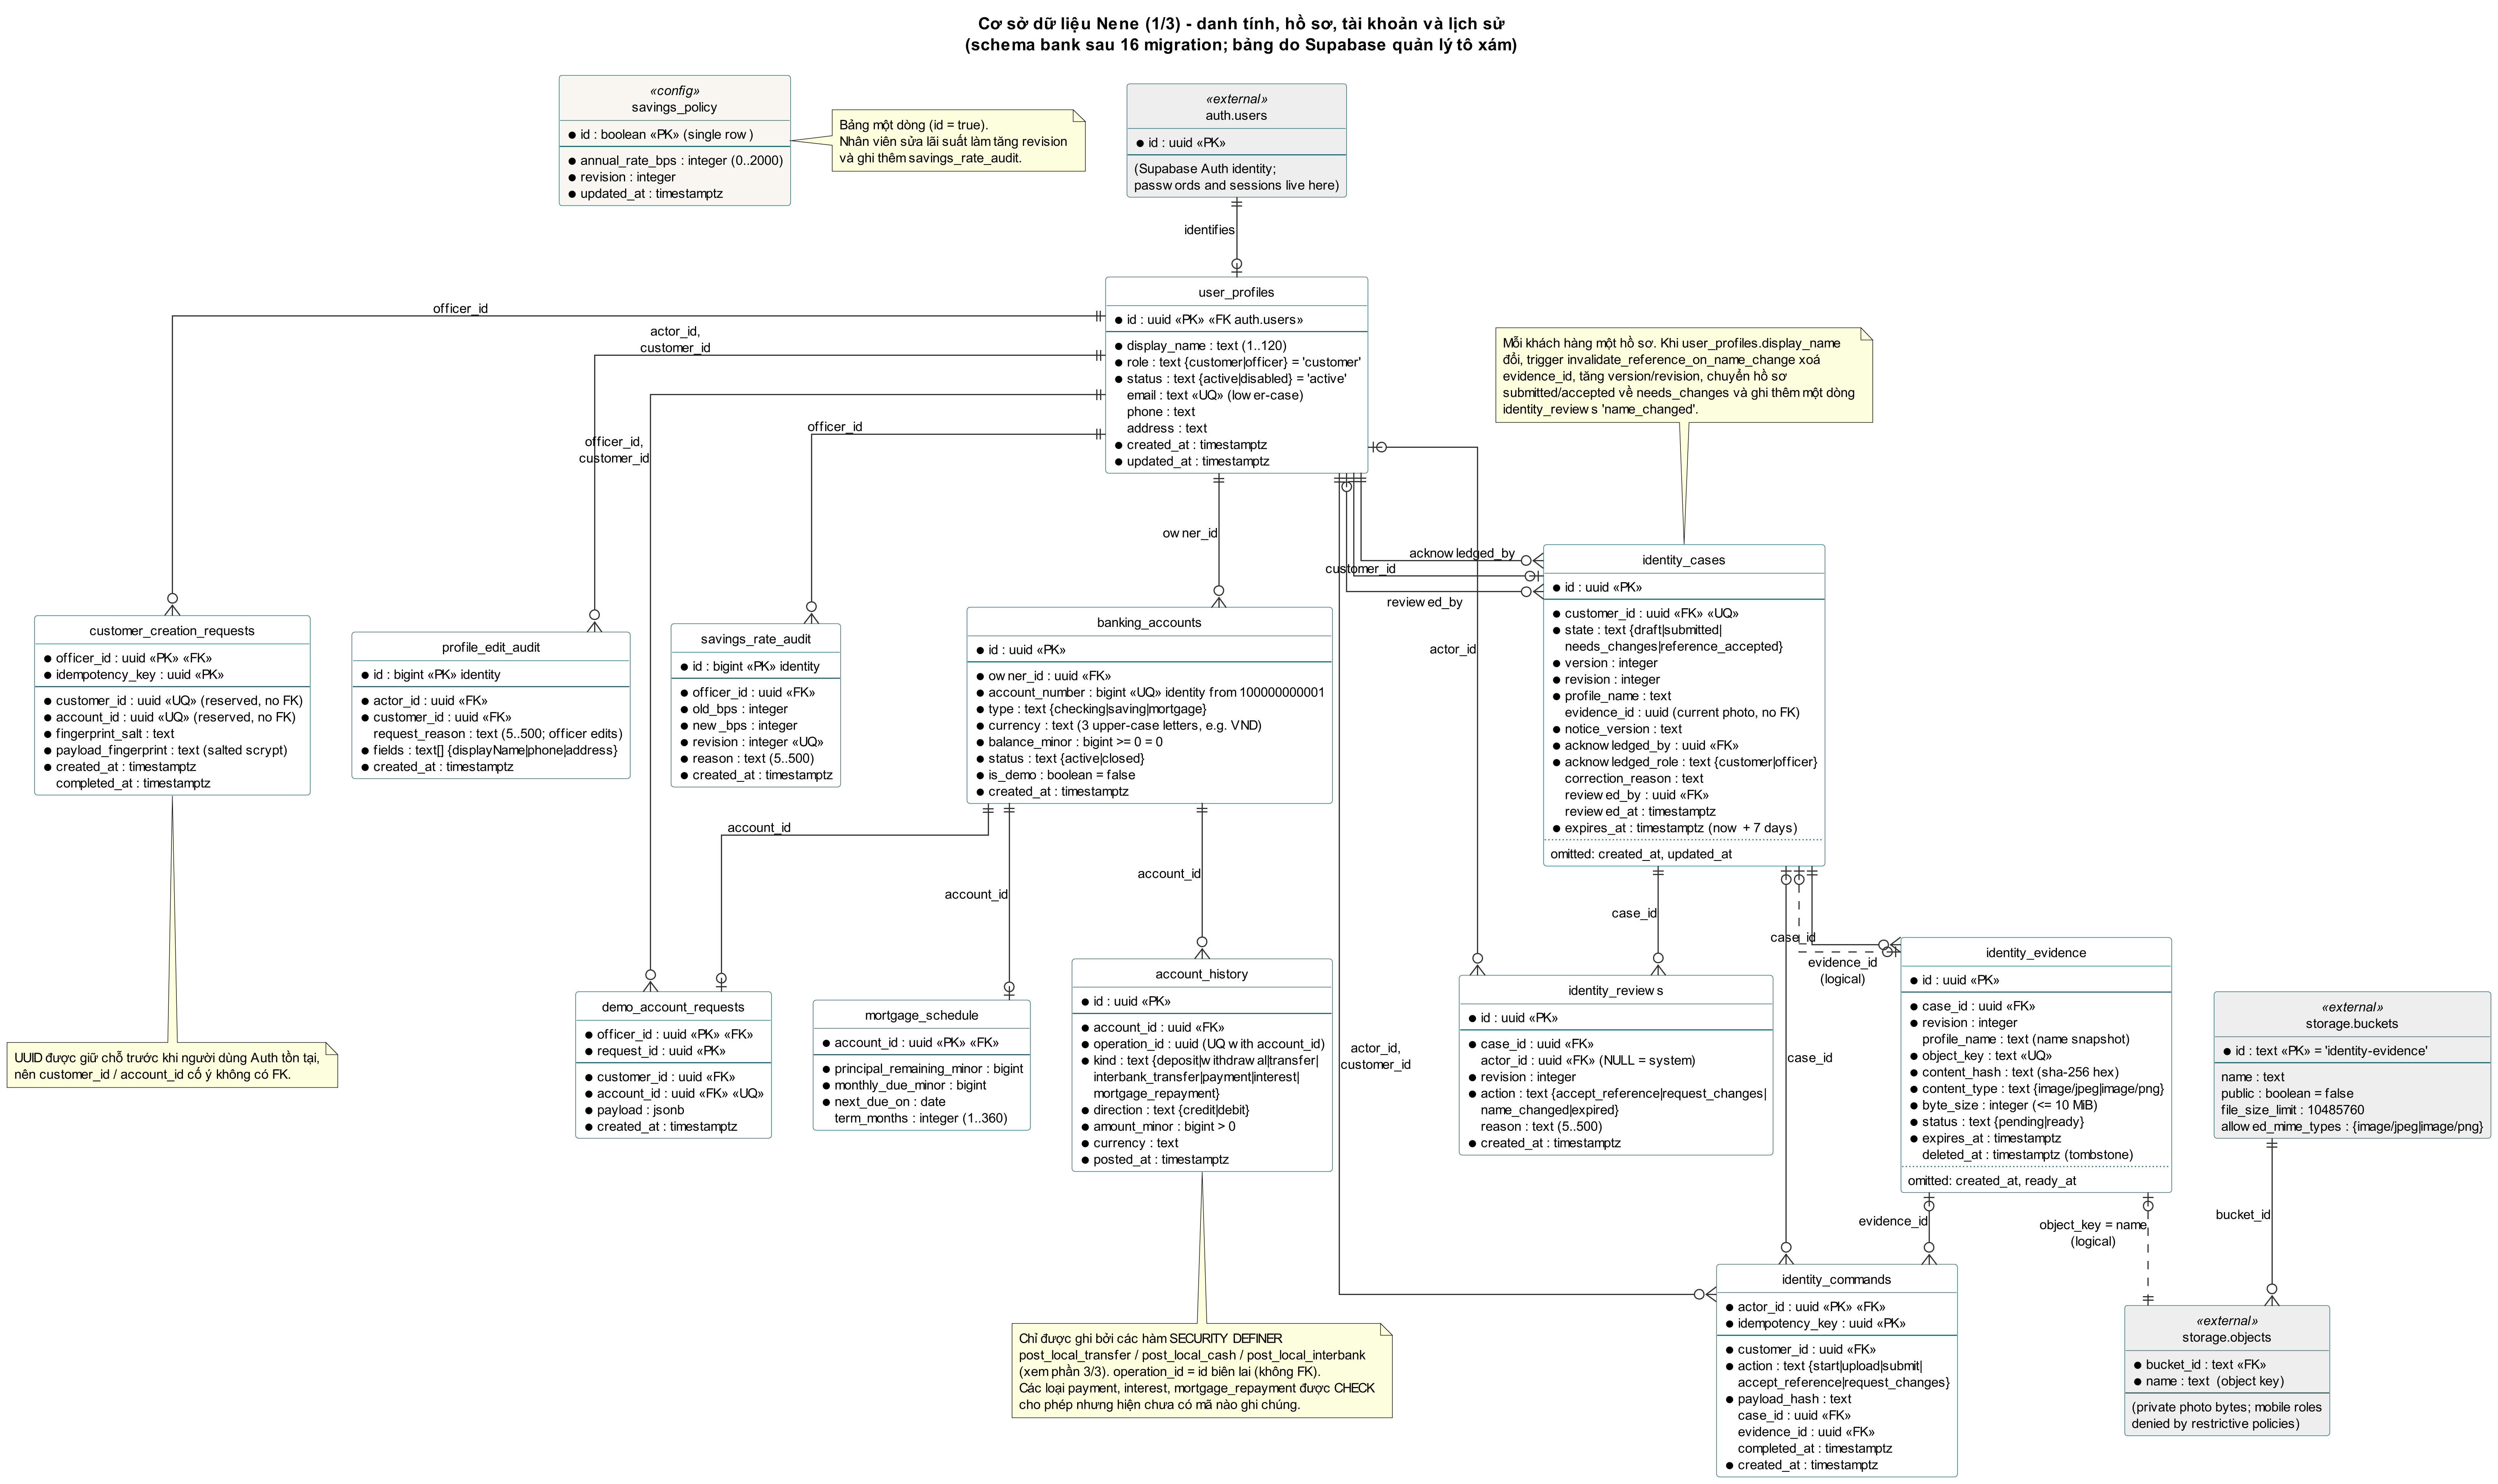
\includegraphics[angle=90,width=\textwidth,height=0.8\textheight,keepaspectratio]{picture/ch2/er-core}
\caption{Sơ đồ ER (1/3): danh tính, hồ sơ, tài khoản và lịch sử}
\label{fig:ch2-er-core}
\end{figure}

Hình~\ref{fig:ch2-er-core} là lõi của hệ thống. \texttt{auth.\allowbreak{}users} và \texttt{user\_\allowbreak{}profiles} có quan hệ 1--0..1: mỗi hồ sơ ứng dụng dùng chính id của người dùng Auth làm khoá chính, nhưng một người dùng Auth chưa có hồ sơ thì không có quyền gì trong ngân hàng. Một hồ sơ khách hàng sở hữu 0..* \texttt{banking\_\allowbreak{}accounts}; mỗi tài khoản có 0..* dòng \texttt{account\_\allowbreak{}history} và, nếu là tài khoản vay, tối đa một \texttt{mortgage\_\allowbreak{}schedule} (quan hệ 1--0..1 vì khoá chính của lịch cũng là khoá ngoại tới tài khoản). \texttt{savings\_\allowbreak{}policy} là bảng một dòng chứa lãi suất chung; mỗi lần nhân viên sửa thêm một dòng \texttt{savings\_\allowbreak{}rate\_\allowbreak{}audit}. \texttt{profile\_\allowbreak{}edit\_\allowbreak{}audit} tham chiếu hồ sơ hai lần (người sửa và khách hàng bị sửa). Cụm ảnh tham chiếu gồm: mỗi khách hàng có tối đa một \texttt{identity\_\allowbreak{}cases} (\texttt{customer\_\allowbreak{}id} là \texttt{UNIQUE}); một hồ sơ có 0..* \texttt{identity\_\allowbreak{}evidence} (mỗi lần chụp lại tạo revision mới, ảnh cũ thành bản ghi ``bia mộ'' khi bị xoá) và 0..* \texttt{identity\_\allowbreak{}reviews} chỉ được thêm, không sửa; \texttt{identity\_\allowbreak{}cases.\allowbreak{}evidence\_\allowbreak{}id} trỏ logic tới ảnh hiện hành. \texttt{identity\_\allowbreak{}evidence.\allowbreak{}object\_\allowbreak{}key} liên kết logic với \texttt{storage.\allowbreak{}objects.\allowbreak{}name} trong bucket riêng tư; cơ sở dữ liệu chỉ chứa siêu dữ liệu, không chứa byte ảnh. Hai cột \texttt{customer\_\allowbreak{}id} và \texttt{account\_\allowbreak{}id} của \texttt{customer\_\allowbreak{}creation\_\allowbreak{}requests} cố ý không có khoá ngoại vì UUID được giữ chỗ trước khi người dùng Auth, hồ sơ và tài khoản tồn tại.

\begin{figure}[H]
\centering
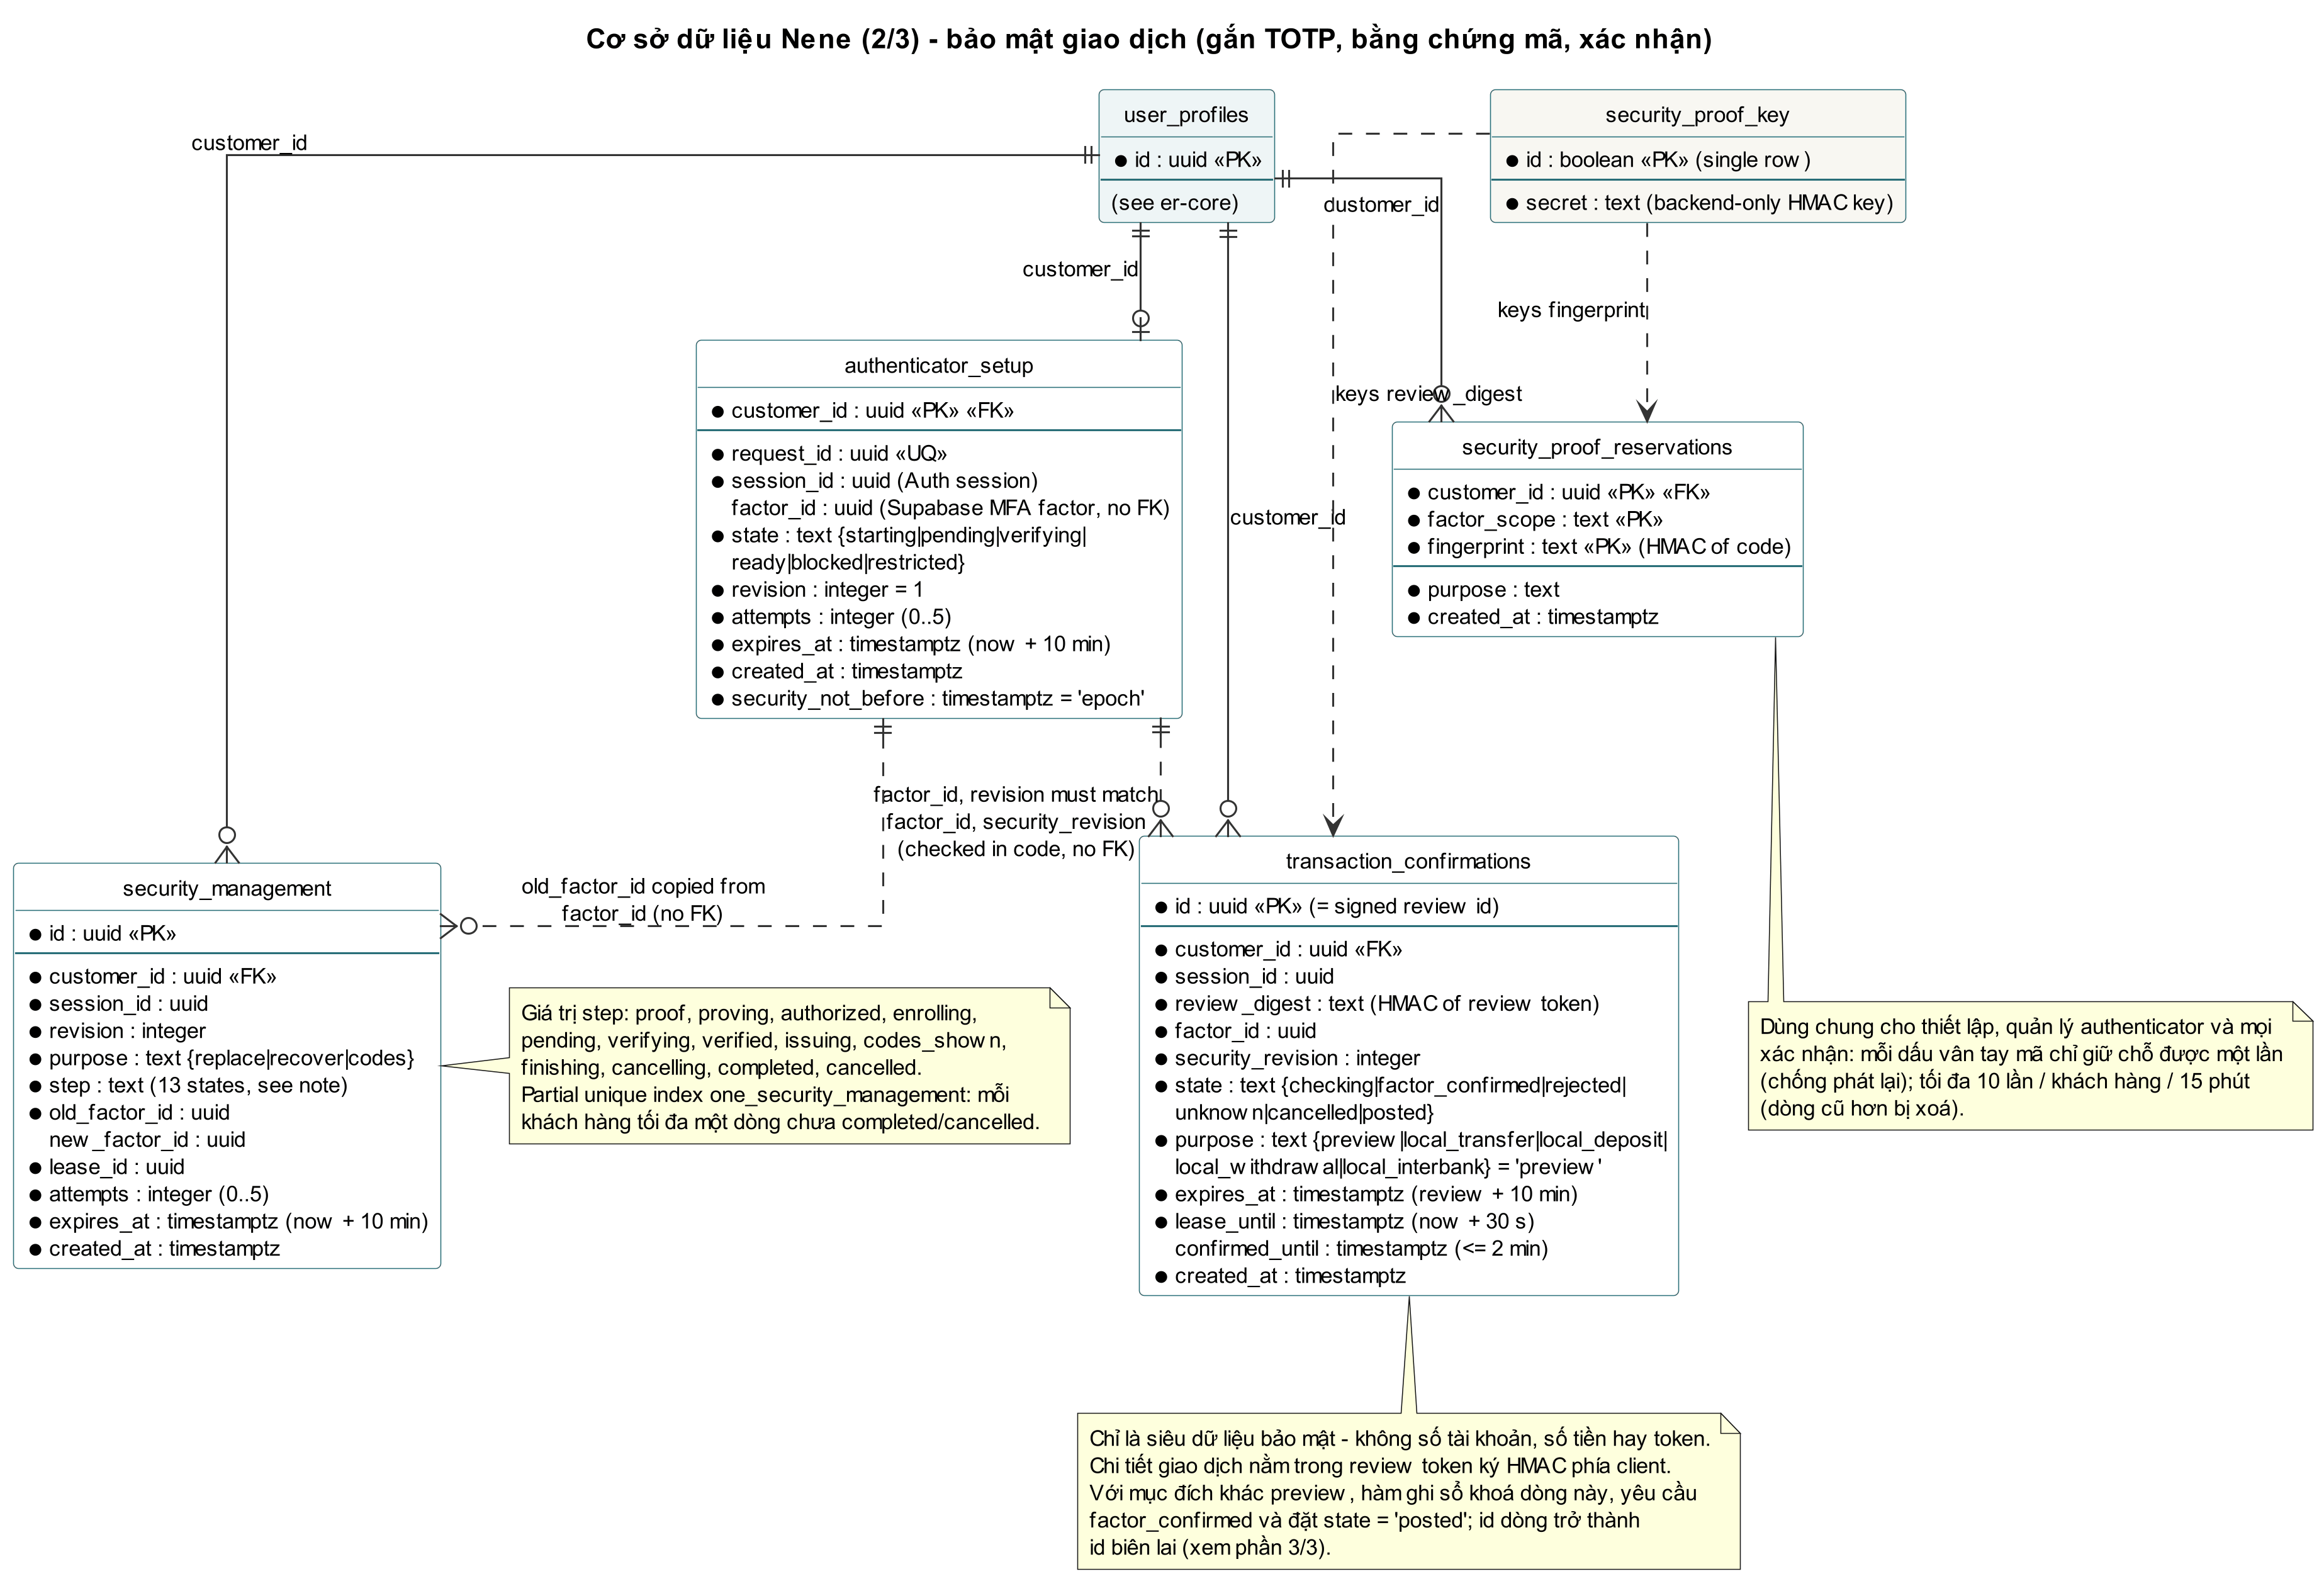
\includegraphics[angle=90,width=\textwidth,height=0.8\textheight,keepaspectratio]{picture/ch2/er-security}
\caption{Sơ đồ ER (2/3): bảo mật giao dịch}
\label{fig:ch2-er-security}
\end{figure}

Hình~\ref{fig:ch2-er-security} gồm các bảng phục vụ BR-04. Mỗi khách hàng có tối đa một \texttt{authenticator\_\allowbreak{}setup} chứa factor TOTP hiện hành và \texttt{revision}; \texttt{transaction\_\allowbreak{}confirmations} sao chép \texttt{factor\_\allowbreak{}id} và \texttt{security\_\allowbreak{}revision} tại lúc xác nhận, và hàm ghi sổ so khớp lại hai giá trị này (liên kết được kiểm tra trong mã, không phải khoá ngoại, vì factor thuộc schema \texttt{auth} của Supabase). \texttt{security\_\allowbreak{}management} lưu tiến trình thay thế/khôi phục authenticator; partial unique index \texttt{one\_\allowbreak{}security\_\allowbreak{}management} đảm bảo mỗi khách hàng có tối đa một tiến trình chưa kết thúc. \texttt{security\_\allowbreak{}proof\_\allowbreak{}key} là bảng một dòng chứa khoá HMAC dùng cho cả dấu vân tay mã (\texttt{security\_\allowbreak{}proof\_\allowbreak{}reservations}) và \texttt{review\_\allowbreak{}digest}. Đáng chú ý, \texttt{transaction\_\allowbreak{}confirmations} chỉ chứa siêu dữ liệu bảo mật: số tài khoản, số tiền và token không được lưu ở đây.

\begin{figure}[H]
\centering
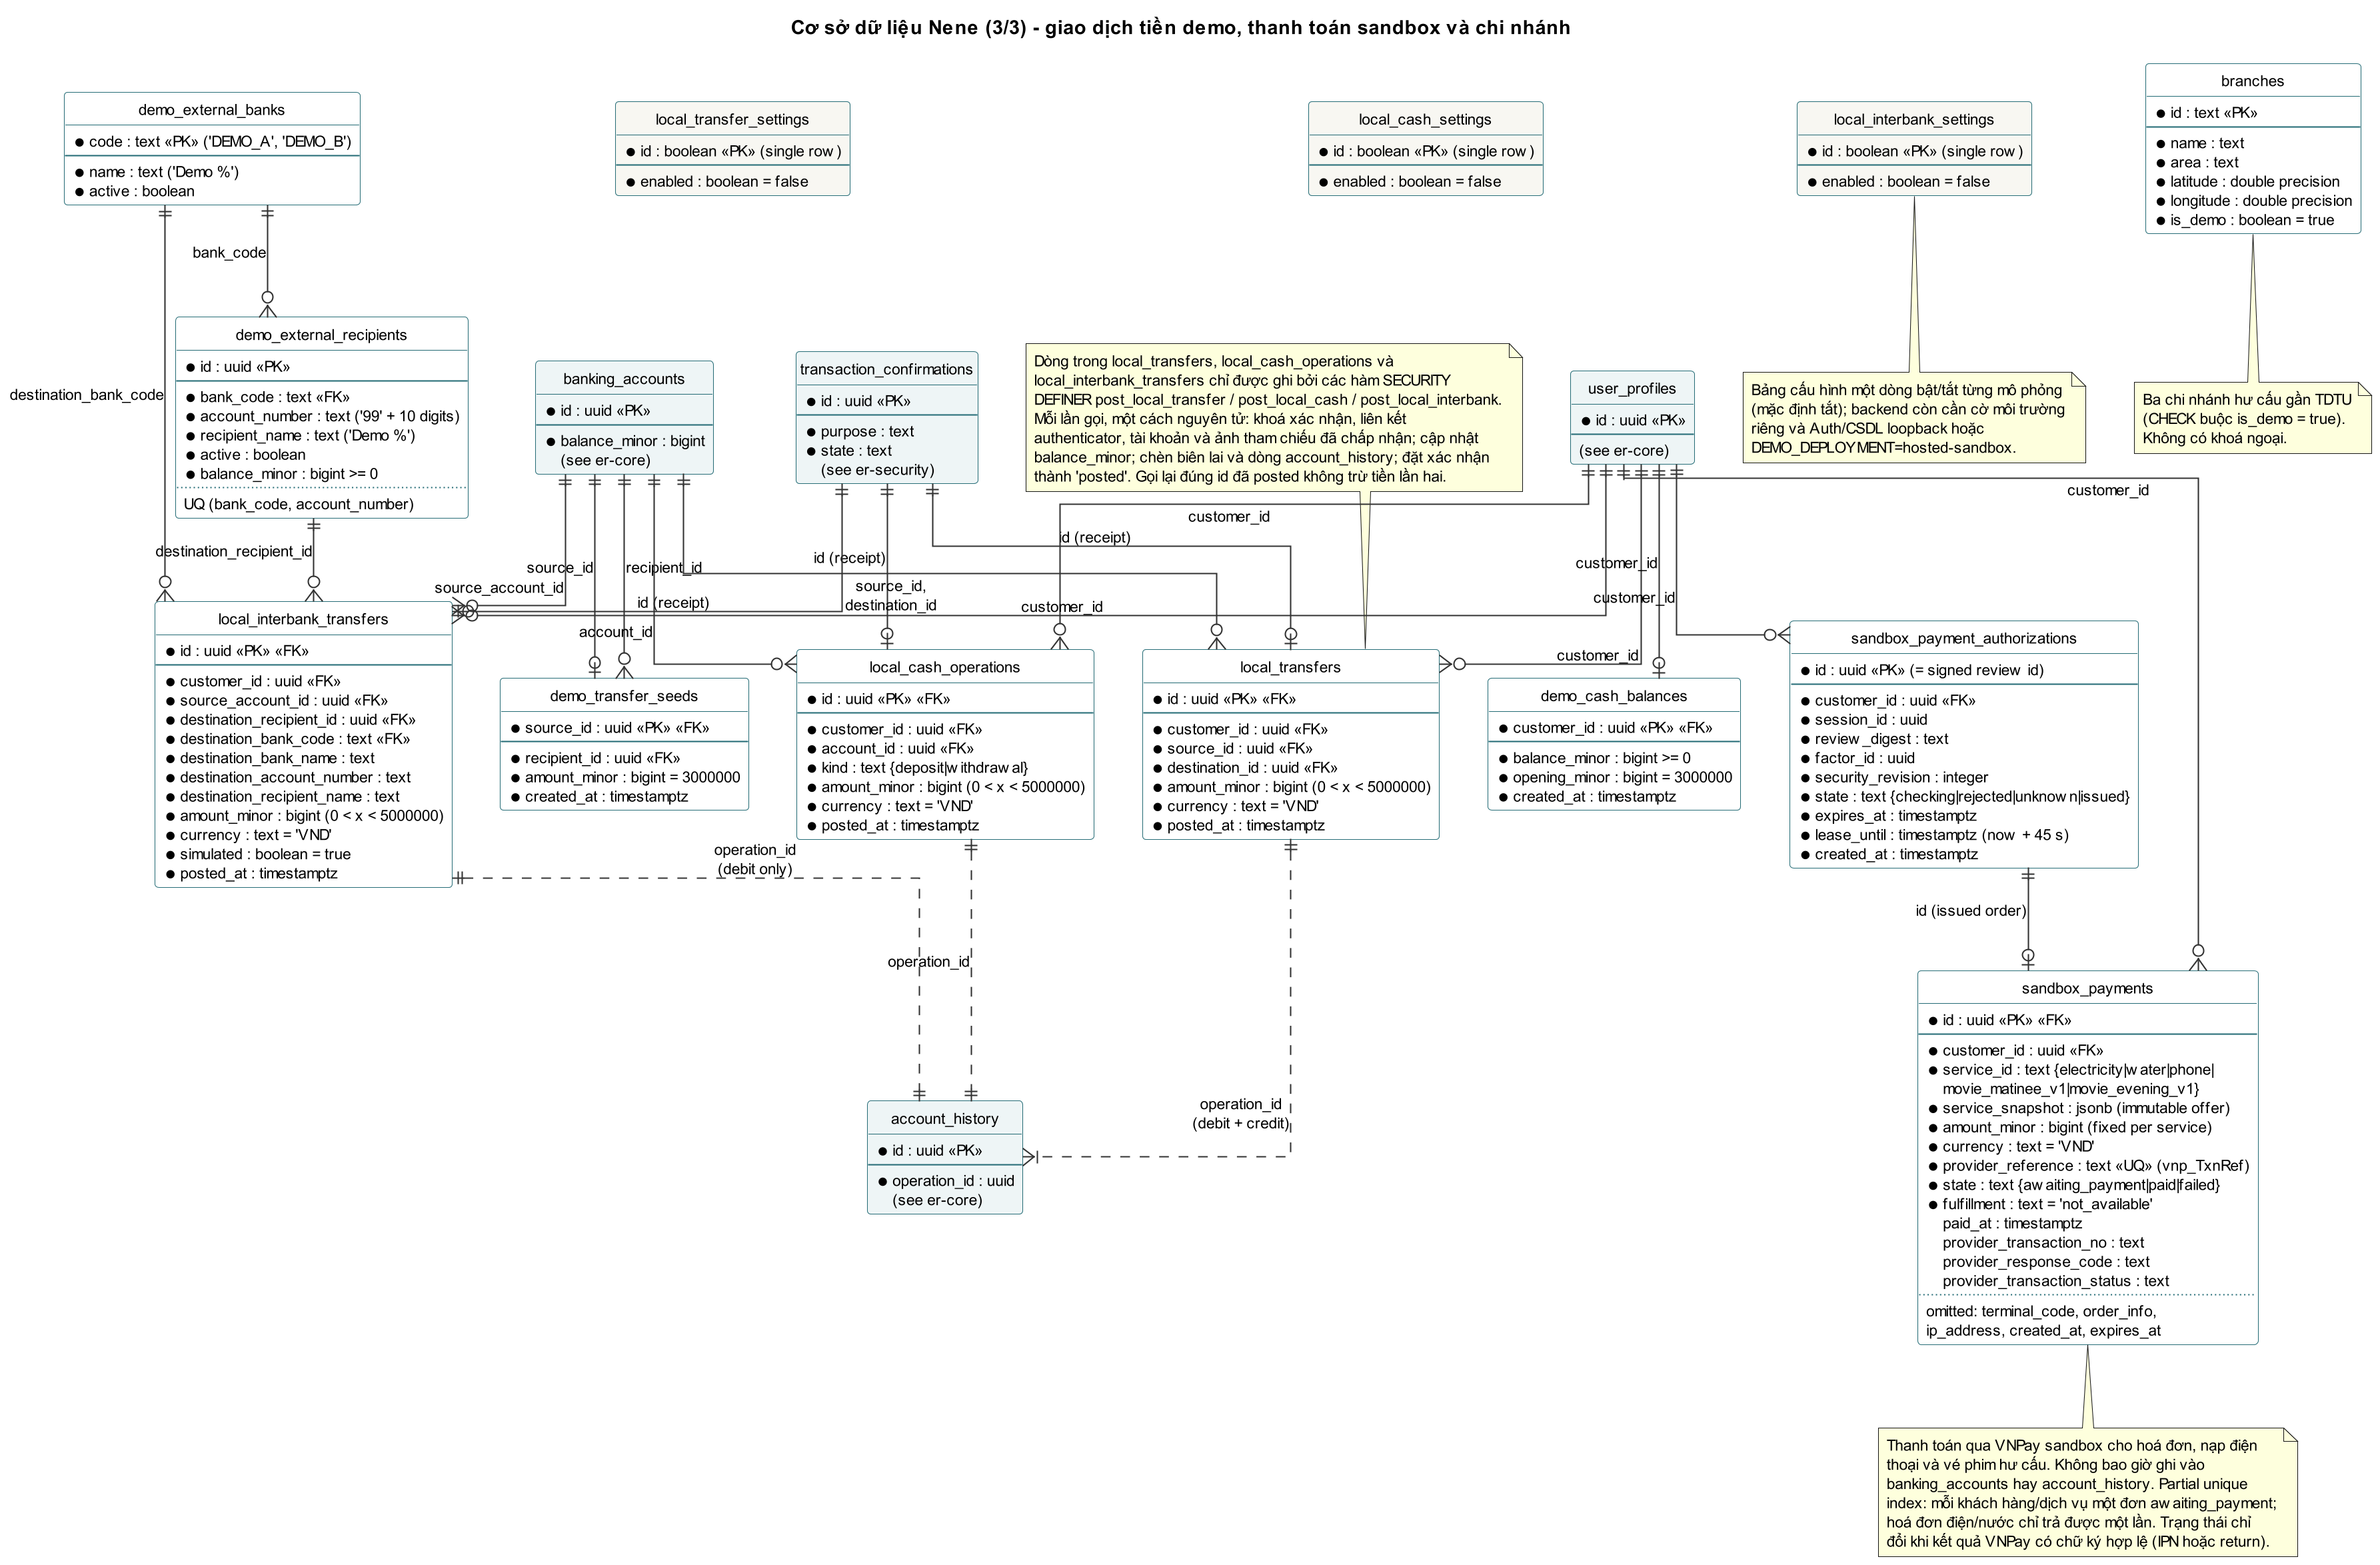
\includegraphics[angle=90,width=\textwidth,height=0.8\textheight,keepaspectratio]{picture/ch2/er-services}
\caption{Sơ đồ ER (3/3): giao dịch tiền demo, thanh toán sandbox và chi nhánh}
\label{fig:ch2-er-services}
\end{figure}

Hình~\ref{fig:ch2-er-services} cho thấy một quy ước thống nhất: khoá chính của mỗi biên lai (\texttt{local\_\allowbreak{}transfers}, \texttt{local\_\allowbreak{}cash\_\allowbreak{}operations}, \texttt{local\_\allowbreak{}interbank\_\allowbreak{}transfers}) đồng thời là khoá ngoại tới \texttt{transaction\_\allowbreak{}confirmations.\allowbreak{}id} (quan hệ 1--0..1). Do đó \emph{không thể} có biên lai nào mà không gắn với đúng một lần xác nhận TOTP, và một lần xác nhận không thể sinh hai biên lai. Mỗi biên lai liên kết logic với các dòng \texttt{account\_\allowbreak{}history} qua \texttt{operation\_\allowbreak{}id}: chuyển khoản trong Nene sinh hai dòng (ghi nợ và ghi có), nạp/rút và chuyển liên ngân hàng sinh một dòng. Người nhận liên ngân hàng thuộc bảng riêng \texttt{demo\_\allowbreak{}external\_\allowbreak{}recipients} (không phải tài khoản Nene) và mỗi người nhận thuộc một \texttt{demo\_\allowbreak{}external\_\allowbreak{}banks}; biên lai còn chụp lại tên ngân hàng, số tài khoản và tên người nhận tại thời điểm chuyển. Nhánh VNPay tương tự: \texttt{sandbox\_\allowbreak{}payments.\allowbreak{}id} là khoá ngoại tới \texttt{sandbox\_\allowbreak{}payment\_\allowbreak{}authorizations.\allowbreak{}id}, nghĩa là chỉ một lần xác nhận TOTP thành công mới tạo được một đơn; bảng này không có quan hệ nào với số dư hay lịch sử. \texttt{branches} là bảng độc lập.

\subsection{Mô tả các bảng}
\label{sec:ch2-tables}

Bảng~\ref{tab:ch2-tables} mô tả toàn bộ 31 bảng của schema \texttt{bank}, được rút ra trực tiếp từ các migration (các ràng buộc \texttt{CHECK} được ghi theo trạng thái sau migration cuối cùng). Ngoài ra migration đầu tiên tạo một dòng trong \texttt{storage.\allowbreak{}buckets}: bucket \texttt{identity-\allowbreak{}evidence} riêng tư, giới hạn 10~MiB, chỉ nhận \texttt{image/\allowbreak{}jpeg} và \texttt{image/\allowbreak{}png}.

{\footnotesize
\begin{longtable}{>{\raggedright\arraybackslash}p{0.25\textwidth}>{\raggedright\arraybackslash}p{0.25\textwidth}>{\raggedright\arraybackslash}p{0.40\textwidth}}
\caption{Mô tả các bảng trong schema \texttt{bank}}\label{tab:ch2-tables}\\
\toprule
\textbf{Bảng} & \textbf{Mục đích} & \textbf{Cột và ràng buộc chính} \\
\midrule
\endfirsthead
\toprule
\textbf{Bảng} & \textbf{Mục đích} & \textbf{Cột và ràng buộc chính} \\
\midrule
\endhead
\bottomrule
\endfoot
\multicolumn{3}{l}{\textit{Hồ sơ và tài khoản}} \\
\texttt{user\_\allowbreak{}profiles} & Hồ sơ ứng dụng của người dùng; vai trò do máy chủ kiểm soát & PK \texttt{id} = FK \texttt{auth.\allowbreak{}users}; \texttt{role} $\in$ \{customer, officer\}; \texttt{status} $\in$ \{active, disabled\}; \texttt{email} chữ thường, duy nhất (partial index); \texttt{phone} 5--32 ký tự, \texttt{address} 1--300 ký tự \\
\texttt{banking\_\allowbreak{}accounts} & Tài khoản ngân hàng của khách hàng & FK \texttt{owner\_\allowbreak{}id}; \texttt{account\_\allowbreak{}number} bigint tự tăng từ 100000000001, duy nhất; \texttt{type} $\in$ \{checking, saving, mortgage\}; \texttt{currency} 3 chữ in hoa; \texttt{balance\_\allowbreak{}minor} $\geq 0$, mặc định 0; \texttt{status} $\in$ \{active, closed\}; \texttt{is\_\allowbreak{}demo}; mỗi khách hàng tối đa một tài khoản demo mỗi loại saving/mortgage \\
\texttt{customer\_creation\_\allowbreak requests} & Giữ chỗ UUID khi nhân viên tạo khách hàng, chống tạo trùng & PK (\texttt{officer\_\allowbreak{}id}, \texttt{idempotency\_\allowbreak{}key}); \texttt{customer\_\allowbreak{}id}, \texttt{account\_\allowbreak{}id} duy nhất, không FK; \texttt{payload\_\allowbreak{}fingerprint} (scrypt có salt, không lưu mật khẩu); \texttt{completed\_\allowbreak{}at} \\
\texttt{profile\_\allowbreak{}edit\_\allowbreak{}audit} & Nhật ký sửa hồ sơ, chỉ thêm & FK \texttt{actor\_\allowbreak{}id}, \texttt{customer\_\allowbreak{}id}; \texttt{fields} $\subseteq$ \{displayName, phone, address\}, 1--3 phần tử; \texttt{request\_\allowbreak{}reason} 5--500 ký tự; RLS: khách hàng tự sửa chỉ được phone/address và không có lý do, nhân viên phải có lý do \\
\texttt{savings\_\allowbreak{}policy} & Lãi suất tiết kiệm chung (một dòng) & PK \texttt{id} boolean \texttt{CHECK(id)}; \texttt{annual\_\allowbreak{}rate\_\allowbreak{}bps} 0--2000; \texttt{revision} \\
\texttt{savings\_\allowbreak{}rate\_\allowbreak{}audit} & Lịch sử đổi lãi suất & FK \texttt{officer\_\allowbreak{}id} (RLS: phải là nhân viên đang hoạt động); \texttt{old\_\allowbreak{}bps}, \texttt{new\_\allowbreak{}bps}; \texttt{revision} duy nhất; \texttt{reason} 5--500 ký tự \\
\texttt{mortgage\_\allowbreak{}schedule} & Lịch trả vay mẫu & PK = FK \texttt{account\_\allowbreak{}id}; \texttt{principal\_\allowbreak{}remaining\_\allowbreak{}minor}, \texttt{monthly\_\allowbreak{}due\_\allowbreak{}minor} $\geq 0$; \texttt{next\_\allowbreak{}due\_\allowbreak{}on}; \texttt{term\_\allowbreak{}months} 1--360; RLS khi chèn: \texttt{monthly\_\allowbreak{}due = principal / term}, tài khoản vay demo VND số dư 0 \\
\texttt{demo\_account\_\allowbreak requests} & Chống trùng khi cấp tài khoản demo & PK (\texttt{officer\_\allowbreak{}id}, \texttt{request\_\allowbreak{}id}); FK \texttt{customer\_\allowbreak{}id}; \texttt{account\_\allowbreak{}id} FK, duy nhất; \texttt{payload} jsonb \\
\texttt{account\_\allowbreak{}history} & Bút toán đã ghi sổ & FK \texttt{account\_\allowbreak{}id}; \texttt{operation\_\allowbreak{}id}; \texttt{kind} $\in$ \{deposit, withdrawal, transfer, interbank\_transfer, payment, interest, mortgage\_repayment\}; \texttt{direction} $\in$ \{credit, debit\}; \texttt{amount\_\allowbreak{}minor} $> 0$; \texttt{UNIQUE(operation\_\allowbreak{}id, account\_\allowbreak{}id)}; index (\texttt{account\_\allowbreak{}id}, \texttt{posted\_\allowbreak{}at} giảm dần, \texttt{id}) \\
\multicolumn{3}{l}{\textit{Ảnh tham chiếu}} \\
\texttt{identity\_\allowbreak{}cases} & Hồ sơ ảnh tham chiếu hiện hành của khách hàng & \texttt{customer\_\allowbreak{}id} FK, duy nhất; \texttt{state} $\in$ \{draft, submitted, needs\_changes, reference\_accepted\}; \texttt{version}, \texttt{revision} $> 0$; \texttt{notice\_\allowbreak{}version}; \texttt{acknowledged\_\allowbreak{}by/\allowbreak{}role}; \texttt{reviewed\_\allowbreak{}by/\allowbreak{}at}; \texttt{expires\_\allowbreak{}at} = now + 60 ngày; \texttt{CHECK}: đã gửi/chấp nhận thì phải có ảnh, đã chấp nhận thì phải có người duyệt \\
\texttt{identity\_\allowbreak{}evidence} & Siêu dữ liệu ảnh trong Storage & FK \texttt{case\_\allowbreak{}id}; \texttt{object\_\allowbreak{}key} duy nhất; \texttt{content\_\allowbreak{}hash} SHA-256; \texttt{content\_\allowbreak{}type} JPEG/PNG; \texttt{byte\_\allowbreak{}size} $\leq$ 10~MiB; \texttt{status} $\in$ \{pending, ready\}; \texttt{profile\_\allowbreak{}name} (bắt buộc khi chèn); \texttt{deleted\_\allowbreak{}at} \\
\texttt{identity\_\allowbreak{}commands} & Chống trùng lệnh ảnh tham chiếu & PK (\texttt{actor\_\allowbreak{}id}, \texttt{idempotency\_\allowbreak{}key}); FK \texttt{customer\_\allowbreak{}id}, \texttt{case\_\allowbreak{}id}, \texttt{evidence\_\allowbreak{}id}; \texttt{action} $\in$ \{start, upload, submit, accept\_reference, request\_changes\}; \texttt{payload\_\allowbreak{}hash} \\
\texttt{identity\_\allowbreak{}reviews} & Quyết định duyệt, chỉ thêm & FK \texttt{case\_\allowbreak{}id}, \texttt{actor\_\allowbreak{}id} (NULL = hệ thống); \texttt{action} $\in$ \{accept\_reference, request\_changes, name\_changed, expired\}; \texttt{CHECK}: hành động hệ thống không có người thực hiện, mọi hành động trừ chấp nhận phải có lý do \\
\multicolumn{3}{l}{\textit{Bảo mật giao dịch}} \\
\texttt{authenticator\_\allowbreak setup} & Factor TOTP hiện hành của khách hàng & PK = FK \texttt{customer\_\allowbreak{}id}; \texttt{request\_\allowbreak{}id} duy nhất; \texttt{factor\_\allowbreak{}id}; \texttt{state} $\in$ \{starting, pending, verifying, ready, blocked, restricted\}; \texttt{revision}; \texttt{attempts} 0--5; hết hạn sau 10 phút \\
\texttt{security\_\allowbreak management} & Tiến trình thay, khôi phục authenticator, cấp mã khôi phục & FK \texttt{customer\_\allowbreak{}id}; \texttt{purpose} $\in$ \{replace, recover, codes\}; \texttt{step} (13 giá trị); \texttt{old/\allowbreak{}new\_\allowbreak{}factor\_\allowbreak{}id}; \texttt{lease\_\allowbreak{}id}; \texttt{attempts} 0--5; tối đa một tiến trình đang mở mỗi khách hàng \\
\texttt{security\_\allowbreak{}proof\_\allowbreak{}key} & Khoá HMAC bí mật phía máy chủ (một dòng) & PK \texttt{id} boolean; \texttt{secret} sinh ngẫu nhiên trong migration; \texttt{nene\_\allowbreak{}api} chỉ đọc \\
\texttt{security\_proof\_\allowbreak reservations} & Chống dùng lại mã & PK (\texttt{customer\_\allowbreak{}id}, \texttt{factor\_\allowbreak{}scope}, \texttt{fingerprint}); \texttt{purpose}; \texttt{created\_\allowbreak{}at} \\
\texttt{transaction\_\allowbreak confirmations} & Một lần xác nhận TOTP cho mỗi review đã ký & PK \texttt{id} = id review; FK \texttt{customer\_\allowbreak{}id}; \texttt{session\_\allowbreak{}id}; \texttt{review\_\allowbreak{}digest}; \texttt{factor\_\allowbreak{}id}; \texttt{security\_\allowbreak{}revision}; \texttt{state} $\in$ \{checking, factor\_confirmed, rejected, unknown, cancelled, posted\}; \texttt{purpose} $\in$ \{preview, local\_transfer, local\_deposit, local\_withdrawal, local\_interbank\}; \texttt{expires\_\allowbreak{}at}, \texttt{lease\_\allowbreak{}until}, \texttt{confirmed\_\allowbreak{}until}; API chỉ được sửa \texttt{state}, \texttt{confirmed\_\allowbreak{}until} \\
\multicolumn{3}{l}{\textit{Giao dịch tiền demo}} \\
\texttt{local\_transfer\_\allowbreak settings} & Bật/tắt chuyển khoản (một dòng) & \texttt{enabled} mặc định \texttt{false}; API chỉ đọc \\
\texttt{demo\_transfer\_\allowbreak seeds} & Ghi nhận khoản tiền mở đầu tổng hợp & PK = FK \texttt{source\_\allowbreak{}id}; FK \texttt{recipient\_\allowbreak{}id}; \texttt{amount\_\allowbreak{}minor} = 3000000; API không có quyền \\
\texttt{local\_\allowbreak{}transfers} & Biên lai chuyển khoản trong Nene & PK = FK \texttt{transaction\_\allowbreak{}confirmations}; FK \texttt{customer\_\allowbreak{}id}, \texttt{source\_\allowbreak{}id}, \texttt{destination\_\allowbreak{}id}; $0 <$ \texttt{amount\_\allowbreak{}minor} $< 5000000$; \texttt{currency} = VND; nguồn khác đích \\
\texttt{local\_cash\_\allowbreak settings} & Bật/tắt nạp/rút mô phỏng (một dòng) & \texttt{enabled} mặc định \texttt{false}; API chỉ đọc \\
\texttt{demo\_\allowbreak{}cash\_\allowbreak{}balances} & Nguồn tiền mặt mô phỏng của mỗi khách hàng & PK = FK \texttt{customer\_\allowbreak{}id}; \texttt{balance\_\allowbreak{}minor} $\geq 0$; \texttt{opening\_\allowbreak{}minor} = 3000000 \\
\texttt{local\_cash\_\allowbreak operations} & Biên lai nạp/rút & PK = FK \texttt{transaction\_\allowbreak{}confirmations}; FK \texttt{customer\_\allowbreak{}id}, \texttt{account\_\allowbreak{}id}; \texttt{kind} $\in$ \{deposit, withdrawal\}; $0 <$ \texttt{amount\_\allowbreak{}minor} $< 5000000$; VND \\
\texttt{local\_interbank\_\allowbreak settings} & Bật/tắt liên ngân hàng mô phỏng (một dòng) & \texttt{enabled} mặc định \texttt{false}; API chỉ đọc \\
\texttt{demo\_external\_\allowbreak banks} & Ngân hàng hư cấu & PK \texttt{code} dạng \texttt{DEMO\_\allowbreak{}*}; \texttt{name} bắt đầu ``Demo''; dữ liệu mẫu \texttt{DEMO\_\allowbreak{}A}, \texttt{DEMO\_\allowbreak{}B} \\
\texttt{demo\_external\_\allowbreak recipients} & Người nhận hư cấu, số dư mô phỏng & FK \texttt{bank\_\allowbreak{}code}; \texttt{account\_\allowbreak{}number} gồm ``99'' và 10 chữ số; \texttt{recipient\_\allowbreak{}name} bắt đầu ``Demo''; \texttt{balance\_\allowbreak{}minor} $\geq 0$; \texttt{UNIQUE(bank\_\allowbreak{}code, account\_\allowbreak{}number)} \\
\texttt{local\_interbank\_\allowbreak transfers} & Biên lai chuyển liên ngân hàng mô phỏng & PK = FK \texttt{transaction\_\allowbreak{}confirmations}; FK tài khoản nguồn, người nhận, ngân hàng; bản chụp tên ngân hàng, số tài khoản, tên người nhận; \texttt{simulated} bị buộc \texttt{true}; $0 <$ \texttt{amount\_\allowbreak{}minor} $< 5000000$; VND \\
\multicolumn{3}{l}{\textit{Thanh toán sandbox và chi nhánh}} \\
\texttt{sandbox\_payment\_\allowbreak authorizations} & Một lần xác nhận TOTP cho mỗi review thanh toán & FK \texttt{customer\_\allowbreak{}id}; \texttt{session\_\allowbreak{}id}; \texttt{review\_\allowbreak{}digest}; \texttt{factor\_\allowbreak{}id}; \texttt{security\_\allowbreak{}revision}; \texttt{state} $\in$ \{checking, rejected, unknown, issued\}; \texttt{lease\_\allowbreak{}until} 45 giây \\
\texttt{sandbox\_\allowbreak{}payments} & Đơn thanh toán VNPay sandbox & PK = FK \texttt{sandbox\_\allowbreak{}payment\_\allowbreak{}authorizations}; \texttt{service\_\allowbreak{}id} $\in$ \{electricity, water, phone, movie\_matinee\_v1, movie\_evening\_v1\} với số tiền cố định (200.000; 100.000; 50.000; 90.000; 120.000 VND); \texttt{provider\_\allowbreak{}reference} duy nhất; \texttt{state} $\in$ \{awaiting\_payment, paid, failed\}; \texttt{fulfillment} = not\_available; \texttt{paid\_\allowbreak{}at} có khi và chỉ khi paid; \texttt{service\_\allowbreak{}snapshot} jsonb được \texttt{CHECK} cấu trúc \\
\texttt{branches} & Chi nhánh hư cấu gần TDTU & PK \texttt{id} text; \texttt{latitude} $-90$..$90$, \texttt{longitude} $-180$..$180$; \texttt{is\_\allowbreak{}demo} bị buộc \texttt{true}; ba dòng mẫu \\
\end{longtable}
}

\subsection{Ràng buộc toàn vẹn}
\label{sec:ch2-integrity}

Nhóm đẩy càng nhiều bất biến nghiệp vụ xuống cơ sở dữ liệu càng tốt, để chúng đúng với mọi đường ghi dữ liệu chứ không chỉ với mã hiện tại:
\begin{itemize}
  \item \textbf{Toàn vẹn thực thể và tham chiếu}: mọi bảng có khoá chính; khoá ngoại dùng \texttt{ON DELETE RESTRICT} (hoặc mặc định \texttt{NO ACTION}), nên không thể xoá một hồ sơ hay tài khoản còn được tham chiếu; lịch sử tài chính không bao giờ bị xoá dây chuyền.
  \item \textbf{Toàn vẹn miền}: \texttt{CHECK} giới hạn tập giá trị của vai trò, trạng thái, loại tài khoản, loại bút toán; độ dài văn bản; dạng mã tiền tệ; khoảng số tiền; cấu trúc JSON của \texttt{service\_\allowbreak{}snapshot}.
  \item \textbf{Ràng buộc liên cột}: ví dụ \texttt{(state = 'paid') = (paid\_\allowbreak{}at is not null)} trong \texttt{sandbox\_\allowbreak{}payments}; \texttt{source\_\allowbreak{}id <> destination\_\allowbreak{}id} trong \texttt{local\_\allowbreak{}transfers}; hồ sơ ảnh đã chấp nhận phải có người duyệt và thời điểm duyệt.
  \item \textbf{Duy nhất có điều kiện (partial unique index)}: mỗi khách hàng tối đa một tài khoản demo mỗi loại tiết kiệm/vay, một tiến trình quản lý authenticator đang mở, một đơn VNPay đang chờ cho mỗi dịch vụ; hoá đơn điện/nước demo chỉ thanh toán được một lần.
  \item \textbf{Trigger}: \texttt{invalidate\_reference\_\allowbreak on\_name\_change} chạy sau khi \texttt{display\_\allowbreak{}name} thay đổi, trong cùng giao dịch với lệnh sửa: xoá liên kết ảnh hiện hành, tăng version/revision, chuyển hồ sơ đã gửi hoặc đã chấp nhận về \texttt{needs\_\allowbreak{}changes} và ghi một dòng \texttt{identity\_\allowbreak{}reviews}. Nhờ vậy không thể có ảnh đã chấp nhận gắn với một cái tên khác.
  \item \textbf{Bảng một dòng}: các bảng cấu hình dùng khoá chính boolean với \texttt{CHECK(id)}, nên chỉ có đúng một dòng.
\end{itemize}

\subsection{Vai trò, phân quyền và bảo mật mức dòng}
\label{sec:ch2-roles}

Cơ chế phân quyền gồm hai lớp. Lớp thứ nhất là \textbf{quyền} (privilege): như đã trình bày ở Mục~\ref{sec:ch2-least-privilege}, mọi quyền trên schema \texttt{bank} bị thu hồi khỏi các vai trò client của Supabase và cả \texttt{service\_\allowbreak{}role}; \texttt{nene\_\allowbreak{}api} có thuộc tính \texttt{NOINHERIT}, \texttt{NOBYPASSRLS} và chỉ nhận những quyền cần thiết, nhiều chỗ ở mức cột. Các bảng cấu hình và biên lai chỉ được cấp \texttt{SELECT}; \texttt{demo\_\allowbreak{}transfer\_\allowbreak{}seeds} không được cấp quyền nào. Lớp thứ hai là \textbf{bảo mật mức dòng} (RLS) \parencite{ch2-pg-rls,ch2-supabase-rls}: RLS được bật và \emph{ép buộc} (\texttt{FORCE ROW LEVEL SECURITY}) trên các bảng nghiệp vụ, kèm chính sách cho \texttt{nene\_\allowbreak{}api}. Nhóm dùng RLS như một lớp kiểm tra cấu trúc bổ sung chứ không phải nơi lọc theo từng người dùng: nhiều chính sách đọc là \texttt{using (true)}, vì việc lọc theo chủ sở hữu được thực hiện ở NestJS bằng định danh đã xác minh. Những chính sách có điều kiện đáng chú ý gồm: chỉ tạo tài khoản số dư 0 cho khách hàng đang hoạt động; chỉ tạo hồ sơ khách hàng với vai trò \texttt{customer}; chỉ nhân viên đang hoạt động mới được ghi nhật ký lãi suất hay duyệt ảnh; khách hàng tự sửa hồ sơ thì chỉ được sửa điện thoại và địa chỉ; lịch vay mẫu phải có khoản trả bằng gốc chia số kỳ. Các bảng không bật RLS là ba bảng cấu hình một dòng và bảng seed, vốn chỉ có quyền đọc hoặc không có quyền nào đối với \texttt{nene\_\allowbreak{}api}; riêng \texttt{authenticator\_\allowbreak{}setup} bật RLS nhưng không ép buộc, điều này không ảnh hưởng tới \texttt{nene\_\allowbreak{}api} vì RLS luôn áp dụng cho vai trò không phải chủ sở hữu bảng.

Với Storage, hai chính sách \emph{restrictive} trên \texttt{storage.\allowbreak{}objects} và \texttt{storage.\allowbreak{}buckets} chặn \texttt{anon} và \texttt{authenticated} khỏi bucket \texttt{identity-\allowbreak{}evidence}; vì là restrictive nên kể cả khi sau này có ai thêm một chính sách cho phép rộng hơn, bucket này vẫn bị chặn với ứng dụng.

\subsection{Biểu diễn tiền tệ và quy tắc tính toán}
\label{sec:ch2-money}

Mọi số tiền được lưu bằng số nguyên \texttt{bigint} theo \emph{đơn vị nhỏ nhất} của tiền tệ (cột có hậu tố \texttt{\_\allowbreak{}minor}), kèm cột \texttt{currency} tường minh. Với VND, đơn vị nhỏ nhất là 1 đồng, nên 5.000.000 VND được lưu là \texttt{5000000}. Cách biểu diễn này loại bỏ sai số làm tròn của số thực dấu phẩy động. Trên đường truyền, API gửi số tiền dưới dạng chuỗi và backend tính bằng \texttt{BigInt} để không mất độ chính xác. Các hàm ghi sổ kiểm tra tràn số (\texttt{balance\_\allowbreak{}minor > 9223372036854775807 - p\_\allowbreak{}amount}) trước khi cộng.
\begin{itemize}
  \item \textbf{Lãi suất tiết kiệm} được lưu theo điểm cơ bản (\texttt{annual\_\allowbreak{}rate\_\allowbreak{}bps}, 1 bps = 0,01\%), giới hạn 0--2000 (0--20\%/năm). Lợi nhuận ước tính một tháng được tính trong \texttt{account-\allowbreak{}information.\allowbreak{}ts}:
  \[
    \text{lợi nhuận tháng} = \left\lfloor \frac{\text{số dư} \times \text{bps} + 60000}{120000} \right\rfloor,
  \]
  tức số dư $\times$ lãi suất năm / 12, làm tròn nửa lên tới đồng. Đây là ước tính hiển thị; hệ thống không tự ghi có tiền lãi.
  \item \textbf{Lịch trả vay thế chấp} là lịch mẫu hằng tháng với lãi suất 0\%: khoản trả định kỳ bằng phần nguyên của gốc chia số tháng (\texttt{monthly\_\allowbreak{}due\_\allowbreak{}minor = principal\_\allowbreak{}remaining\_\allowbreak{}minor / term\_\allowbreak{}months}), số tháng từ 1 đến 360. Chỉ khoản trả định kỳ, dư nợ gốc ban đầu và ngày đến hạn đầu tiên được lưu và hiển thị; hệ thống chưa xử lý trả nợ hay tự chuyển kỳ. Số tiền mỗi hai tuần không được lưu mà được backend tính từ khoản trả hằng tháng: cùng tổng số tiền một năm chia cho 26 kỳ, làm tròn lên tới đồng, tức $\lceil \text{khoản tháng} \times 12 / 26 \rceil$, tính bằng số nguyên \texttt{BigInt}. Đây là cách hiển thị quy đổi, không phải một lịch trả nợ hai tuần riêng.
  \item \textbf{Ngưỡng giá trị cao}: mọi giao dịch tiền và thanh toán phải nhỏ hơn 5.000.000 VND (\texttt{CHECK} trong bảng và kiểm tra trong hàm). Đây là quyết định của dự án: đề bài yêu cầu dùng ảnh khuôn mặt để xác minh hoạt động giá trị cao, nhưng Nene chưa có so khớp khuôn mặt tự động, nên thay vì cho phép giao dịch lớn mà không xác minh, hệ thống chặn hẳn. Để tham khảo, Quyết định 2345/QĐ-NHNN của Ngân hàng Nhà nước yêu cầu xác thực sinh trắc học cho giao dịch chuyển tiền trực tuyến trên 10 triệu đồng mỗi lần hoặc tổng trên 20 triệu đồng mỗi ngày \parencite{ch5-sbv2345}; ngưỡng của Nene thấp hơn mức này.
\end{itemize}

% ======================================================================
\section{Thiết kế các luồng xử lý quan trọng}
\label{sec:ch2-flows}

\subsection{Chuyển khoản trong Nene}
\label{sec:ch2-flow-transfer}

Hình~\ref{fig:ch2-seq-transfer} là biểu đồ tuần tự của chuyển khoản giữa hai tài khoản thanh toán VND trong Nene, luồng tiêu biểu cho mọi giao dịch tiền (nạp, rút và liên ngân hàng mô phỏng đi theo cùng khuôn mẫu, chỉ khác hàm ghi sổ cuối cùng).

\begin{figure}[H]
\centering
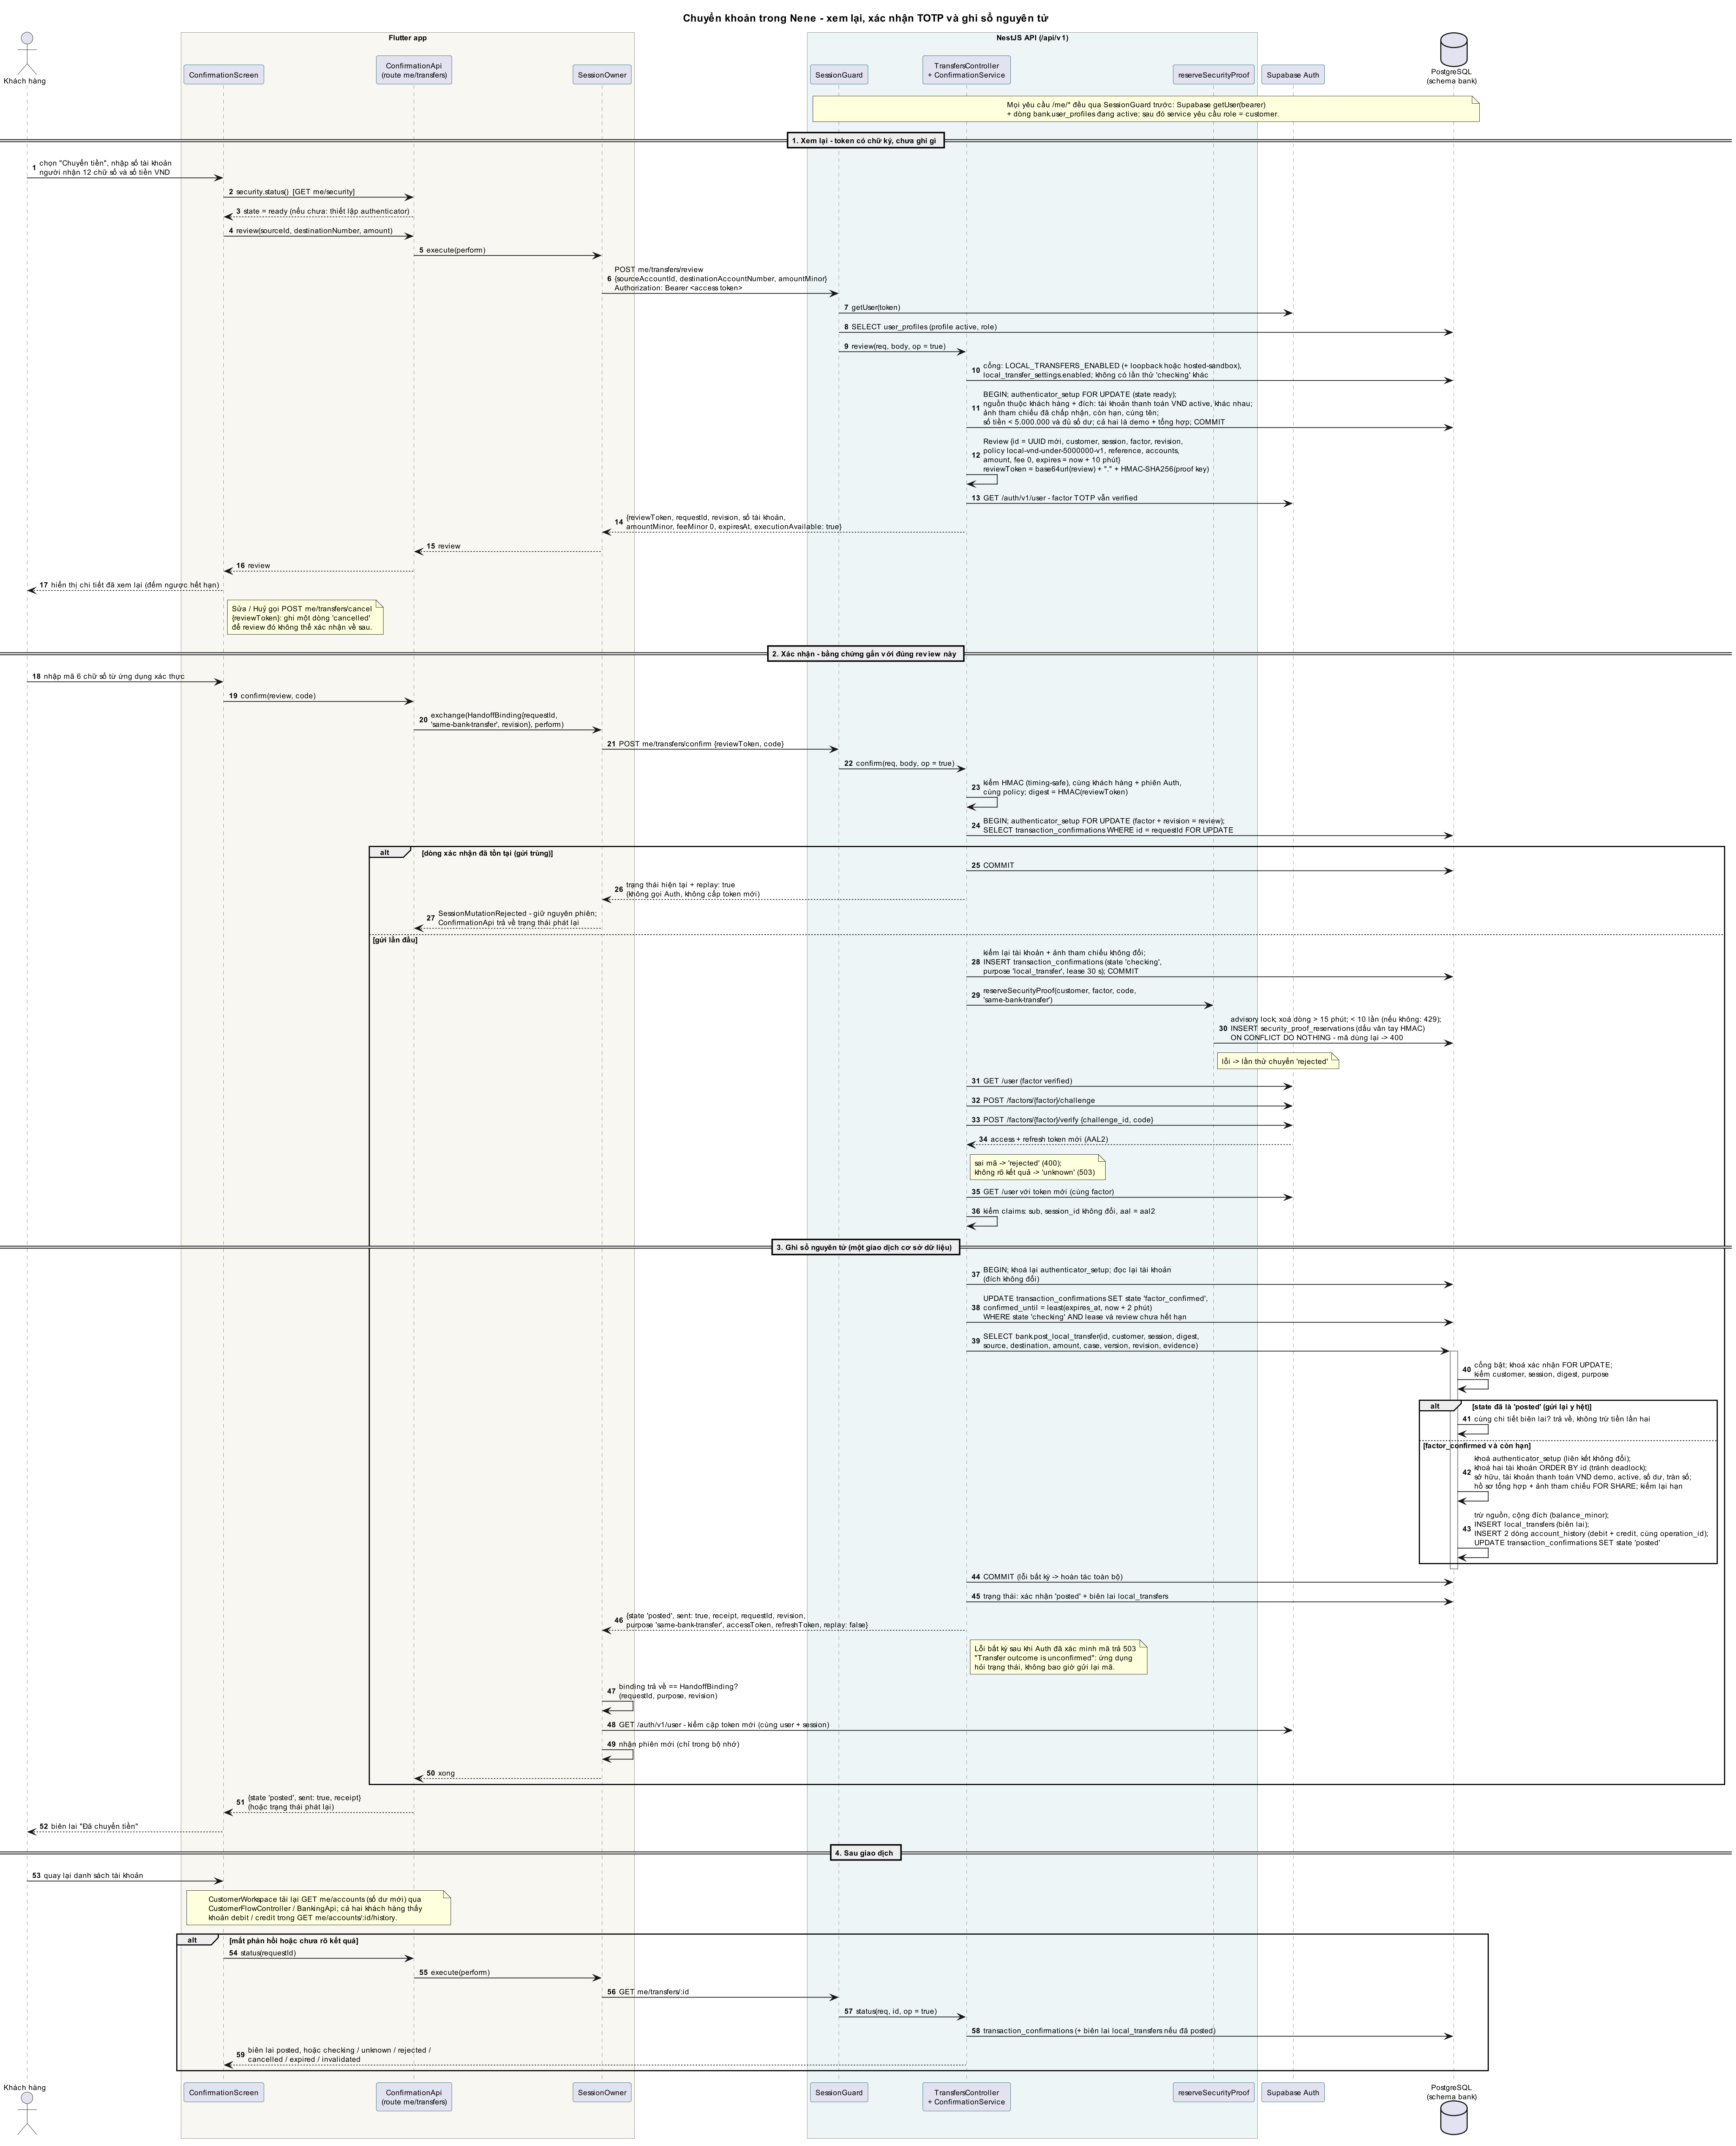
\includegraphics[width=\textwidth,height=0.85\textheight,keepaspectratio]{picture/ch2/seq-transfer}
\caption{Biểu đồ tuần tự chuyển khoản: xem lại, xác nhận TOTP và ghi sổ nguyên tử}
\label{fig:ch2-seq-transfer}
\end{figure}

Các bước chính (số trong ngoặc là số thứ tự thông điệp trên biểu đồ):
\begin{enumerate}
  \item \textbf{Kiểm tra điều kiện trước} (1--3). Khách hàng chọn tài khoản nguồn, nhập số tài khoản người nhận 12 chữ số và số tiền. Ứng dụng kiểm tra authenticator đã ở trạng thái \texttt{ready}; nếu chưa, khách hàng được dẫn tới màn hình thiết lập.
  \item \textbf{Xem lại} (4--17). Ứng dụng gửi \texttt{POST me/\allowbreak{}transfers/\allowbreak{}review}. Sau \texttt{SessionGuard}, \texttt{Confirmation\allowbreak{}Service} kiểm tra cờ bật luồng, rồi trong một giao dịch đọc: khoá \texttt{authenticator\_\allowbreak{}setup}, xác nhận tài khoản nguồn thuộc khách hàng, tài khoản đích tồn tại và khác nguồn, cả hai là tài khoản thanh toán VND demo đang hoạt động của khách hàng tổng hợp, ảnh tham chiếu đã được chấp nhận và còn hạn, số tiền nhỏ hơn 5.000.000 và đủ số dư. Service tạo đối tượng \texttt{Review} với UUID mới và thời hạn 10 phút rồi ký HMAC. \emph{Chưa có gì được ghi vào cơ sở dữ liệu}. Ứng dụng hiển thị chi tiết kèm đồng hồ đếm ngược; nếu khách hàng sửa hoặc huỷ, \texttt{POST me/\allowbreak{}transfers/\allowbreak{}cancel} ghi một dòng \texttt{cancelled} để review đó không thể được xác nhận về sau.
  \item \textbf{Xác nhận} (18--36). Khách hàng nhập mã 6 chữ số. Ứng dụng gọi \texttt{SessionOwner.\allowbreak{}exchange()} với \texttt{Handoff\allowbreak{}Binding} của review. Backend kiểm tra chữ ký, khách hàng, phiên Auth và policy; nếu đã có dòng xác nhận cho review này (gửi trùng) thì trả trạng thái hiện tại với \texttt{replay: true} mà không gọi Supabase. Nếu là lần đầu, backend kiểm tra lại tài khoản và ảnh tham chiếu, chèn \texttt{transaction\_\allowbreak{}confirmations} trạng thái \texttt{checking}, giữ chỗ dấu vân tay mã, rồi gọi Supabase Auth: lấy factor, tạo challenge, xác minh mã. Mã sai làm lần thử chuyển \texttt{rejected} (HTTP 400); không rõ kết quả thì chuyển \texttt{unknown} (HTTP 503). Khi thành công, backend kiểm tra phiên mới có \texttt{aal2} và cùng \texttt{session\_\allowbreak{}id}.
  \item \textbf{Ghi sổ nguyên tử} (37--46). Trong \emph{một} giao dịch cơ sở dữ liệu, backend khoá lại liên kết authenticator, đặt xác nhận thành \texttt{factor\_\allowbreak{}confirmed} với \texttt{confirmed\_\allowbreak{}until} tối đa 2 phút, rồi gọi \texttt{bank.\allowbreak{}post\_\allowbreak{}local\_\allowbreak{}transfer}. Hàm kiểm tra lại toàn bộ điều kiện dưới khoá (Mục~\ref{sec:ch2-atomic}), trừ tiền nguồn, cộng tiền đích, chèn biên lai \texttt{local\_\allowbreak{}transfers}, chèn hai dòng lịch sử (ghi nợ và ghi có, cùng \texttt{operation\_\allowbreak{}id}) và đặt xác nhận thành \texttt{posted}. Bất kỳ lỗi nào làm toàn bộ giao dịch hoàn tác. Nếu xác nhận đã ở \texttt{posted} (gửi lại y hệt), hàm chỉ so khớp chi tiết biên lai và trả về mà không trừ tiền lần hai.
  \item \textbf{Nhận phiên mới và biên lai} (47--52). \texttt{SessionOwner} chỉ nhận cặp token AAL2 mới khi binding trả về khớp và đã được kiểm tra lại với Supabase Auth; ứng dụng hiển thị biên lai ``Đã chuyển tiền''.
  \item \textbf{Khôi phục khi mất phản hồi} (53--59). Nếu phản hồi bị mất hoặc backend trả lỗi ``kết quả chưa xác nhận'' sau khi mã đã được Supabase chấp nhận, ứng dụng \emph{không bao giờ gửi lại mã} mà gọi \texttt{GET me/\allowbreak{}transfers/\allowbreak{}:id} để đọc trạng thái thật: \texttt{posted} kèm biên lai, hoặc \texttt{checking}, \texttt{unknown}, \texttt{rejected}, \texttt{cancelled}, \texttt{expired}, \texttt{invalidated}. Sau giao dịch, danh sách tài khoản và lịch sử của cả hai khách hàng phản ánh khoản ghi nợ và ghi có.
\end{enumerate}

\subsection{Thanh toán qua VNPay sandbox}
\label{sec:ch2-flow-vnpay}

Luồng thanh toán hoá đơn, nạp điện thoại và mua vé phim dùng chung một quy trình. Mọi dịch vụ đều hư cấu và chạy trên môi trường sandbox của VNPay; không hoá đơn thật nào được thanh toán, không điện thoại nào được nạp tiền, không vé thật nào được phát hành, và số dư Nene không thay đổi.
\begin{enumerate}
  \item \textbf{Chọn dịch vụ}. Ứng dụng đọc \texttt{GET me/\allowbreak{}payments/\allowbreak{}configuration}: danh mục dịch vụ cố định do máy chủ quy định (điện 200.000, nước 100.000, nạp điện thoại 50.000, hai suất phim 90.000 và 120.000 VND) và cờ cho biết thanh toán có được cấu hình hay không.
  \item \textbf{Xem lại có chữ ký}. \texttt{POST me/\allowbreak{}payments/\allowbreak{}review} kiểm tra khách hàng tổng hợp đang hoạt động, ảnh tham chiếu đã chấp nhận và còn hạn, authenticator \texttt{ready}, rồi trả review token ký HMAC-SHA256 (thời hạn 10 phút) gắn khách hàng, phiên, dịch vụ, số tiền, factor/revision, phiên bản ảnh tham chiếu và mã yêu cầu.
  \item \textbf{Xác nhận TOTP và tạo đơn}. \texttt{POST me/\allowbreak{}payments/\allowbreak{}confirm} chèn \texttt{sandbox\_\allowbreak{}payment\_\allowbreak{}authorizations} (\texttt{checking}), giữ chỗ dấu vân tay mã, xác minh mã với Supabase, kiểm tra lại các điều kiện, rồi trong một giao dịch đặt xác nhận thành \texttt{issued} và chèn một đơn \texttt{sandbox\_\allowbreak{}payments} trạng thái \texttt{awaiting\_\allowbreak{}payment} với \texttt{provider\_\allowbreak{}reference} duy nhất và bản chụp bất biến của dịch vụ. Phiên AAL2 mới được nhận qua \texttt{SessionOwner.\allowbreak{}exchange()} với mục đích \texttt{vnpay-\allowbreak{}checkout}.
  \item \textbf{Ký URL thanh toán}. \texttt{create\allowbreak{}Sandbox\allowbreak{}Checkout} (\texttt{backend/\allowbreak{}src/\allowbreak{}payments/\allowbreak{}vnpay.\allowbreak{}ts}) dựng các tham số VNPay PAY 2.1.0 (\texttt{vnp\_\allowbreak{}Command=pay}, \texttt{vnp\_\allowbreak{}Amount} = số VND $\times$ 100, \texttt{vnp\_\allowbreak{}TxnRef}, thời gian theo UTC+07, cửa sổ thanh toán 15 phút), sắp xếp và mã hoá tham số rồi ký HMAC-SHA512 bằng khoá bí mật của terminal \parencite{ch2-vnpay-pay}. Khoá này chỉ nằm ở backend.
  \item \textbf{Thanh toán trên VNPay}. Ứng dụng kiểm tra URL đúng máy chủ và đường dẫn HTTPS của sandbox rồi mở trình duyệt ngoài. Khách hàng thanh toán bằng thẻ thử nghiệm; mã OTP của ngân hàng thử nghiệm là bước riêng của VNPay, tách biệt với TOTP của Nene.
  \item \textbf{Nhận và xác minh kết quả}. VNPay báo kết quả qua hai đường: IPN (máy chủ gọi máy chủ, \texttt{GET payments/\allowbreak{}vnpay/\allowbreak{}ipn}) và chuyển hướng trình duyệt về \texttt{GET payments/\allowbreak{}vnpay/\allowbreak{}return}. Cả hai đều đi vào cùng hàm \texttt{Payments\allowbreak{}Service.\allowbreak{}ipn()}: phân tích chuỗi truy vấn gốc, từ chối tham số trùng hoặc sai định dạng, tính lại HMAC-SHA512 và so sánh an toàn thời gian, kiểm tra mã terminal; sau đó trong một giao dịch khoá đơn theo \texttt{provider\_\allowbreak{}reference}, so khớp terminal, nội dung đơn và số tiền, yêu cầu đơn còn \texttt{awaiting\_\allowbreak{}payment} và lần xác nhận đã \texttt{issued}. Kết quả thành công (mã phản hồi và trạng thái giao dịch đều \texttt{00}) đặt đơn thành \texttt{paid}; trạng thái \texttt{02} đặt thành \texttt{failed}; kết quả lặp lại trả mã ``đơn đã được xác nhận'' mà không đổi gì. Trang return là một trang HTML cố định, không phản chiếu tham số nào, có Content-Security-Policy chặt và chỉ báo ``đã nhận kết quả'' khi kết quả có chữ ký hợp lệ đã được ghi.
  \item \textbf{Kiểm tra trạng thái}. Khách hàng quay lại ứng dụng và xem \texttt{GET me/\allowbreak{}payments/\allowbreak{}:id}.
\end{enumerate}
Lý do xử lý kết quả ở cả trang return: terminal sandbox của nhóm không đăng ký được URL IPN (biểu mẫu đăng ký sandbox không có trường này), nên trên thực tế kết quả được ghi qua đường return, bằng cùng bộ xác minh chữ ký như IPN. Ngày 25/11/2026 nhóm đã chạy thử thật trên sandbox: hai lần thanh toán bằng thẻ thử nghiệm được ghi nhận \texttt{paid}.

\subsection{Đăng ký ảnh tham chiếu khuôn mặt}
\label{sec:ch2-flow-reference}

Luồng này hỗ trợ một phần BR-03. Cần nói rõ giới hạn: đây \emph{không phải} eKYC hoàn chỉnh. Hệ thống không so khớp khuôn mặt, không kiểm tra người thật (liveness), không kiểm tra giấy tờ; trạng thái \texttt{reference\_\allowbreak{}accepted} chỉ có nghĩa là một nhân viên đã xác nhận ảnh thuộc về khách hàng đó.
\begin{enumerate}
  \item \textbf{Bắt đầu}. Khách hàng (hoặc nhân viên cho một khách hàng đã chọn) mở mục ảnh tham chiếu, đọc thông báo phiên bản \texttt{reference-\allowbreak{}demo-\allowbreak{}v2} về mục đích, quyền truy cập riêng tư và thời hạn lưu, xác nhận đã đọc và tạo hồ sơ nháp (\texttt{draft}). Hồ sơ hết hạn sau 60 ngày.
  \item \textbf{Chụp ảnh và kiểm tra trên thiết bị}. Ứng dụng chụp ảnh bằng camera. Trên Android, ML Kit phát hiện khuôn mặt ngay trên thiết bị, ảnh không được gửi đi để kiểm tra: ảnh chỉ được dùng khi có đúng một khuôn mặt với cạnh ngắn của khung mặt chiếm ít nhất 20\% cạnh ngắn của ảnh; không có mặt, nhiều mặt hoặc mặt quá nhỏ thì ảnh bị bỏ và khách hàng được nhắc chụp lại. Trên web/desktop không có bộ phát hiện, và nếu bộ phát hiện lỗi thì ảnh vẫn được phép kèm ghi chú. Đây là phát hiện khuôn mặt, không phải nhận dạng; máy chủ chấp nhận mọi ảnh hợp lệ nên bước này chỉ giúp chụp ảnh dùng được, không phải biện pháp bảo mật.
  \item \textbf{Tải lên riêng tư}. Ảnh được gửi tới \texttt{POST identity/\allowbreak{}cases/\allowbreak{}:id/\allowbreak{}evidence} kèm \texttt{Idempotency-\allowbreak{}Key}. Backend giữ chỗ một dòng \texttt{identity\_\allowbreak{}evidence} (\texttt{pending}, khoá đối tượng do máy chủ sinh, bản chụp tên hiện tại), giải mã và mã hoá lại ảnh bằng \texttt{sharp} (một khung JPEG/PNG, tối đa 4096 $\times$ 4096 điểm ảnh, tối đa 10~MiB, loại bỏ EXIF/GPS), tính SHA-256, ghi vào bucket riêng tư rồi đánh dấu \texttt{ready}.
  \item \textbf{Gửi duyệt}. Khách hàng gửi; hồ sơ chuyển sang \texttt{submitted}.
  \item \textbf{Nhân viên duyệt}. Nhân viên xem ảnh (ảnh đi qua NestJS với \texttt{Cache-\allowbreak{}Control: no-\allowbreak{}store}, không có URL công khai), xác nhận liên kết giữa ảnh và khách hàng để chấp nhận (\texttt{reference\_\allowbreak{}accepted}), hoặc yêu cầu chụp lại kèm lý do 5--500 ký tự (\texttt{needs\_\allowbreak{}changes}). Mỗi quyết định thêm một dòng \texttt{identity\_\allowbreak{}reviews}; \texttt{version} ngăn hai nhân viên ghi đè quyết định của nhau.
  \item \textbf{Vô hiệu hoá và dọn dẹp}. Đổi tên khách hàng làm trigger chuyển hồ sơ về \texttt{needs\_\allowbreak{}changes}; hết hạn 60 ngày cũng làm ảnh không còn dùng được. Ảnh hết hạn hoặc treo ở \texttt{pending} quá 24 giờ được xoá vật lý bằng lệnh bảo trì \texttt{npm run identity:cleanup}, chạy thủ công chứ không phải dịch vụ xoá liên tục.
  \item \textbf{Sử dụng}. Mọi hàm ghi sổ và thanh toán yêu cầu ảnh tham chiếu đã chấp nhận, còn hạn, cùng tên với hồ sơ và ảnh còn ở trạng thái \texttt{ready}. Vì chưa có so khớp khuôn mặt cho từng giao dịch, giao dịch từ 5.000.000 VND trở lên bị chặn; so khớp khuôn mặt tự động là hướng phát triển tiếp theo.
\end{enumerate}

\section{Tóm tắt chương}
\label{sec:ch2-summary}

Chương này đã phân tích hai tác nhân con người, bốn hệ thống bên ngoài và hai mươi ca sử dụng chính gắn với các yêu cầu BR; trình bày kiến trúc client--server gồm ứng dụng Flutter, một API NestJS triển khai trên Render và Supabase (PostgreSQL, Auth, Storage), cùng lý do chọn từng công nghệ so với các phương án khác, đặc biệt là PostgreSQL thay cho Firebase để có ràng buộc quan hệ, giao dịch ACID và phân quyền chi tiết. Các nguyên tắc cốt lõi --- máy chủ là nguồn sự thật, đặc quyền tối thiểu với \texttt{nene\_\allowbreak{}api}, ghi sổ nguyên tử bằng hàm \texttt{SECURITY DEFINER}, khoá chống trùng, TOTP gắn với từng giao dịch, phiên chỉ trong bộ nhớ và ghi nhãn rõ mô phỏng --- được thể hiện nhất quán qua bảy biểu đồ lớp, ba sơ đồ ER với 31 bảng và các luồng xử lý chuyển khoản, thanh toán VNPay sandbox và ảnh tham chiếu. Các giới hạn được nêu rõ: ảnh tham chiếu không phải eKYC hoàn chỉnh, giao dịch giá trị cao bị chặn, chuyển khác ngân hàng và tiền mặt là mô phỏng, dịch vụ thanh toán là hư cấu trên VNPay sandbox. Chi tiết hiện thực và giao diện được trình bày ở Chương~\ref{chap:3}.
